        % ===== INICIO DEL PREÁMBULO =====
%
\documentclass[grd,twoside,openright]{udelar} % Poner msc para Maestría, dsc para Doctorado.
%
\usepackage[
acronyms, 											 % Utiliza el glosario de acronimos.
nohypertypes={acronym,notacion,simbolos,glosario},   % Quita los links en el texto al glosario.
%nonumberlist,                                       % Quita los links en los glosarios al texto.
nogroupskip,                                         % Quita los espacios entre diferentes grupos dentro de un glosario.
nopostdot 											 % Quita el punto final en los acrónimos.
]{glossaries}

\hypersetup{ colorlinks = true } % Hipervínculos: escribir "false" para imprimir o "true" para ver en digital.
 
% Cargar estilo bibliográfico copiando del documento "Estilos bibliográficos UdelaRTeX.pdf"
% \usepackage[backend=biber,style=apa,sortcites,natbib=true]{biblatex}
\usepackage[backend=biber,style=numeric,sortcites,natbib=true,maxbibnames=10]{biblatex}
\DeclareFieldFormat{urldate}{(Accedido el #1)}
% \usepackage{estilos_bibliograficos/udelartex_apa}

% Algorithms
% \usepackage[ruled,vlined]{algorithm2e}
\usepackage[ruled,noline,linesnumbered,spanish]{algorithm2e}
\usepackage{algorithmic}
\usepackage{multirow}
\usepackage{subcaption}
\usepackage{minted}




\addbibresource{bibliografia/biblio_1.bib} % Agregar la cantidad de archivos .bib que se tengan para la bibliografía.
\addbibresource{bibliografia/biblio_2.bib} % Se coloca una línea por archivo .bib.

\loadglossary % No comentar esta línea

% A su vez, la clase udelar.cls ya tiene los siguientes paquetes cargados automáticamente, que podrían ser de interés saber para el usuario:
%{color},{hyphenat},{appendix},{lastpage},{babel},{inputenc},{amsmath,amssymb},{ifthen},{graphicx},{caption}{setspace},{tabularx},{eqparbox},{ltxcmds},{titletoc},{xcolor},{lineno},{xwatermark}

% Si se quieren agregar más paquetes, se recomienda colocarlos a partir de esta linea y antes de \begin{document}.
% ===========  INICIO PAQUETES ===============

% ===========   FIN PAQUETES   ===============


% =====  FIN DEL PREÁMBULO  =====

% ===== INICIO DEL DOCUMENTO =====

\begin{document}
  %
  \title{Particionamiento óptimo de matrices dispersas}
%   \subtitle{Subtítulo de la tesis}
  \institutelogo{1} % Carga cantidad de logos seleccionados, con máximo de 3 logos. Si se pone un logo horizontal, colocar 1 o 2 logos para no desconfigurar la portada.
  \author{Raúl Ignacio}{Marichal}
  \escritura{en} % Se indica que el programa de Posgrado sea "en" o "de" tal área.
  %
 
%   \director{Prof.}{Nombre del Director de Tesis}{Apellido}{D.Sc.} % Comentar esta línea si se tiene solo un director de tesis.
  \codirector{}{Ernesto}{Dufrechou}{Dr. Ing.}  % Comentar estas líneas si no son necesarias.
   \codirector{}{Pablo}{Ezzatti}{Dr. Ing.}
%   \codirector{Prof.}{Nombre del 2do Codirector}{Apellido}{D.Sc.}
%   \codirector{Prof.}{Nombre del 3er Codirector}{Apellido}{D.Sc.}
%   \directoracademico{}{Nombre del Director Académico de Tesis}{Apellido}{D.Sc.}
  %
  \examiner{Prof.}{Nombre del 1er Examinador}{Apellido}{D.Sc.}
  \examiner{Prof.}{Nombre del 2do Examinador}{Apellido}{Ph.D.}
  \examiner{Prof.}{Nombre del 3er Examinador}{Apellido}{D.Sc.}
%   \examiner{Prof.}{Nombre del 4to Examinador}{Apellido}{Ph.D.}
%   \examiner{Prof.}{Nombre del 5to Examinador}{Apellido}{Ph.D.} % Comentar los que no son necesarios.
  %
  \graduatename{Ingeniería en Computación}
  \institute{Facultad de Ingeniería}{FIng}  % La primer institución es la principal.
%   \institute{Facultad de Medicina}{FMed}  % Agregar copias de esta línea para agregar instituciones.
%   \institute{Facultad de Agronomía}{FAgro}  % Agregar copias de esta línea para agregar instituciones. No se discrimina de que universidad es tal facultad.
%   \seconduniversity{Universidad XXXXX} % Se agrega el nombre de otra universidad. Comentar esta linea si no es necesaria.
%   \thirduniversity{Universidad YYYYY} % Se agrega el nombre de otra universidad. Comentar esta linea si no es necesaria.
  \graduatelocation{Montevideo}{Uruguay}
  %
  \date{3}{19}{2021} % Fecha del documento: día/mes/año
  % Palabras claves en español
  \keyword{matrices dispersas}
  \keyword{almacenamiento óptimo}
  \keyword{reordenamiento}
  \keyword{múltiples precisiones}
%   \keyword{5ta palabra clave}
  % Palabras claves en inglés
  \foreignkeyword{1st keyword}
  \foreignkeyword{2nd keyword}
  \foreignkeyword{3rd keyword}
  \foreignkeyword{4th keyword}
  \foreignkeyword{5th keyword}
  %     
  \maketitle  % Comando que genera el título de la tesis.
  %
  \frontmatter  % Comando que genera la portadilla, el catalogo y el tribunal de evaluación. NO COMENTAR
  %
%   \dedication{(Dedicatoria) A alguien cuyo valor es digno de ella.}


  \chapter*{Agradecimientos}

Quisiera agradecer, en primer lugar, a mis hermanos y al resto de mi familia que me apoyó y motivó durante todo mi proceso educativo. 
Agradezco, también a todas las personas de que una manera u otra, me brindaron su apoyo, compartiendo su valioso tiempo, a veces recursos, para ayudarme a que continúe. 
Además quiero dar las gracias a mis amigos, que supieron escucharme y compartir, a veces desde la distancia entendiendo cuando no pude acompañarlos.
He de agradecer también, a las instituciones, Fondo de Solidaridad y Bienestar Universitario, que me brindaron apoyo financiero a lo largo de la carrera
de no haber contado con ellas, hubiese sido, sin duda, mucho más difícil llegar hasta aquí.

Sin quitarles mérito, quisiera agradecer a mis tutores,
Ernesto y Pablo, por su apoyo y guía durante todo el proceso, siendo un pilar importantísimo para la finalización del proyecto, motivándome a siempre seguir adelante, incluso cuando creía haber perdido la fuerza de voluntad.


  %\epigrafe{{\normalfont{(Epígrafe:)}} Frase que alude al tema de trabajo.}{Autor}


  \begin{abstract}
Las matrices dispersas tienen múltiples aplicaciones en el ámbito de la ciencia y la ingeniería, ya que son una herramienta fundamental para la resolución de problemas de gran escala que no pueden ser modelados por matrices densas como, por ejemplo, las simulaciones de circuitos electrónicos, la resolución de ecuaciones diferenciales parciales utilizando FEM, o incluso operaciones con grafos de redes sociales. La creciente importancia de las matrices dispersas para la comunidad científica motiva el estudio de técnicas que permitan el manejo eficiente, tanto del almacenamiento como del cómputo de las operaciones asociadas con este tipo de matrices.
En general, estas técnicas buscan reducir el tráfico de datos con la memoria principal mediante formatos de almacenamiento que permitan ubicar los elementos no nulos dentro de la matriz transfiriendo la menor cantidad de datos posibles.

% Considerando lo expresado anteriormente, 
El objetivo principal de este proyecto es avanzar en el estudio y comprensión de estas estrategias. En particular, se evalúan estrategias de particionamiento y procesamiento de matrices para el uso eficiente de técnicas de almacenamiento centradas, principalmente, en la aplicación de reordenamientos, el uso de múltiples precisiones para almacenar los índices de los elementos no nulos y formatos híbridos que permitan almacenar la matriz mediante una parte regular, en general densa, y una parte irregular dispersa. El trabajo incluye, en primer lugar, la actualización del estado del arte respecto a formatos de almacenamiento disperso. Luego se  desarrollaron un conjunto  de heurísticas que tienen por objetivo optimizar el espacio de almacenamiento de las matrices dispersas mediante el particionamiento de las mismas, alcanzando resultados alentadores.
Por último, se extendió la evaluación experimental midiendo el impacto de la compresión de índices luego de aplicar los reordenamientos.
Este estudio permitió identificar los importantes ahorros en cuanto a espacio de almacenamiento que se pueden obtener al comprimir índices y, además, resaltó la importancia de combinar estrategias de reordenamiento para dicha tarea.

\end{abstract}


%   \begin{foreignabstract}

In this work, we present ...

\end{foreignabstract}
  %
%  \listoffigures	         % Lista de figuras
%  \listoftables	         % Lista de tablas
%   \listadesimbolos 		 % Lista de símbolos
%   \listadenotaciones 	     % Lista de notaciones
%   \listadesiglas 		     % Lista de siglas
  %
  \tableofcontents           % Tabla de contenidos. Compilar dos veces para ver los cambios completos.
  %
  \mainmatter % Comando que genera las listas y capítulos. NO COMENTAR
  % 

  % Agregar archivo de macros
  \newcommand{\resumen}[1]{{\it #1}}

\newcommand{\deposito}[1]{{}}

  \newcommand{\nnz}{\textit{nnz }}
% \newcommand{\bw}{$\beta$}
\newcommand{\bw}{\textit{BW}}
\newcommand{\dc}{\textit{DC}}



  % \algnewcommand\algorithmicforeach{\textbf{for each}}
% \algdef{S}[FOR]{ForEach}[1]{\algorithmicforeach\ #1\ \algorithmicdo}

  % Se incluyen los capítulos. Se pueden comentar los capítulos en los cuales no se está trabajando, para que el documento de trabajo sea más pequeño y compile más rápido.
  \chapter{Introducción}\label{ch:intro}

% \resumen{Motivación}

Las matrices dispersas son aquellas que poseen una fracción relativamente pequeña (frecuentemente muy menor al 1\%) de sus coeficientes distintos a cero, lo que motiva el uso de estructuras de almacenamiento que aprovechen esta particularidad. Específicamente, se suelen almacenar únicamente los coeficientes distintos de cero, acompañados por índices que permitan deducir sus coordenadas en la matriz. Su importancia en el ámbito de la ciencia y la ingeniería radica en que son una herramienta fundamental para la resolución de problemas de gran escala que no pueden ser modelados por matrices densas, por ejemplo, algunos problemas de optimización~\cite{Gill1984} o la resolución de ecuaciones diferenciales parciales utilizando el Método de Elementos Finitos (o FEM por Finite Element Method)~\cite{Saad2003}. Los FEMs~\cite{klaus-jürgenbathe2014} permiten resolver ecuaciones diferenciales asociadas a un problema físico sobre geometrías complicadas (por ejemplo \cite{audi-piston-rod}). Son usados en el diseño y mejora de productos y aplicaciones industriales, así como en la simulación de sistemas físicos y biológicos complejos. La variedad de problemas a los que puede aplicarse ha crecido enormemente, siendo el requisito básico que las ecuaciones constitutivas y ecuaciones de evolución temporal del problema sean conocidas de antemano, representadas comúnmente a la hora de resolverlas como matrices dispersas. Una completa revisión del uso de matrices dispersas en la computación científica, en las etapas tempranas de desarrollo, hasta el año 1977, se puede encontrar en el trabajo de I. Duff~\cite{Duff1977}.

En los últimos años, las matrices dispersas han ido cobrando cada vez más relevancia en el campo de la computación científica, debido, por ejemplo, al impulso del crecimiento de las aplicaciones relacionadas con las redes sociales. En este contexto, las matrices representan, en general, un grafo de las relaciones entre los diferentes usuarios, tal como se presenta en \cite{Hummon1990}, alcanzando matrices de dimensiones extraordinariamente grandes y, al mismo tiempo, con muy pocos coeficientes no nulos.


Esta evolución, descrita en los párrafos anteriores, motiva el estudio de técnicas eficientes, tanto desde el punto de vista del almacenamiento como del cómputo de las operaciones asociadas a las matrices dispersas. 
% Además, considerando la diversidad de problemas donde se usan estas estructuras de datos, las características de las matrices son muy diferentes. Esta situación dificulta aún más avanzar en dicho desarrollo.
Dado que las características de estas matrices, como pueden ser su tamaño, la proporción de elementos distintos de cero o la posición de los mismos, varían fuertemente según la aplicación, esta área de trabajo se encuentra aún en constante desarrollo.


Uno de los principales desafíos que presentan los problemas con matrices dispersas (a través de operaciones como la multiplicación matriz dispersa-vector -SpMV-) es que, en su gran mayoría, son inherentemente limitados por los accesos a memoria, por lo que mejorar la forma de almacenar las matrices para optimizar las comunicaciones de datos entre la memoria y el procesador es crucial. En este caso, suelen ser útiles las técnicas de ordenamiento que permiten reorganizar los coeficientes no nulos de la matriz de forma que éstos puedan almacenarse de manera más eficiente. Otra de las ideas interesantes que apuntan a optimizar el trabajo con matrices dispersas, son aquellas que intentan reducir la precisión de los elementos almacenados, reduciendo las comunicaciones con la memoria. Hartwig Anzt et al.~\cite{Grtzmacher2019}, por ejemplo, presenta estrategias enfocadas en almacenar los coeficientes en punto flotante de precisión adaptable. Sin embargo, parte importante de las comunicaciones en problemas dispersos están dedicadas al manejo de los índices que permiten direccionar dichos coeficientes. Por este motivo es interesante explorar técnicas que permitan, al menos para ciertos tipos de matriz dispersa, almacenar dichos índices de una forma más eficiente. Algunos de los esfuerzos se centran en lograr comprimirlos, aplicando codificaciones distintas, por ejemplo, el delta encoding~\cite{smith1997}. Otros intentan agrupar elementos contiguos y direccionarlos con un índice. Como último punto, presenta un gran interés el hecho de combinar las estrategias antes mencionadas, estudiando la aplicación de ordenamientos  con una posterior compresión de índices.


En el contexto descrito anteriormente, el objetivo de este proyecto es avanzar en el estudio y comprensión de estrategias de optimización de uso de matrices dispersas. En particular, se busca evaluar estrategias de particionamiento y procesamiento de matrices para el uso eficiente de técnicas de almacenamiento. Para alcanzar el objetivo general del proyecto se plantean los siguientes objetivos específicos: 
\begin{itemize}
    \item Actualizar el estado del arte del uso de matrices dispersas.
    \item Actualizar el estado del arte del uso de computación de alta performance (HPC) y en especial, su uso para acelerar la resolución de problemas de álgebra lineal numérica (ALN) dispersa.
    \item Estudiar las técnicas híbridas, reordenamientos y el uso de múltiples precisiones para matrices dispersas.
    \item Desarrollar estrategias (formatos, procedimientos, etc.) para matrices dispersas que permitan alcanzar un uso más eficiente de los datos/cómputo.
\end{itemize}

El resto del documento se estructura de la forma que se describe a continuación.
El Capítulo \ref{ch:fundamento-teorico} presenta, de forma acotada, los conceptos y la teoría en la que está basada este proyecto. Entre otros temas, se aportan detalles sobre matrices dispersas, la multiplicación Matriz dispersa-Vector (SpMV), estrategias de reordenamiento de matrices y hardware para HPC.
En el Capítulo~\ref{ch:estado-del-arte} se resumen los principales antecedentes relacionados con el uso de formatos de almacenamiento de matrices dispersas, el uso de múltiples precisiones y las técnicas de reordenamiento de matrices asociadas.
Posteriormente, en el Capítulo~\ref{ch:propuestas}, se presentan los esfuerzos realizados en el contexto del proyecto de grado. Esto incluye el estudio de técnicas de reordenamiento para formatos híbridos y la evaluación de técnicas de múltiples precisiones. 
El documento se cierra con un resumen de las conclusiones arribadas durante el desarrollo del proyecto y la identificación de líneas de trabajo para continuar el esfuerzo en el Capítulo~\ref{ch:conclusion}.


% Este material busca ser un apoyo a quienes escriben sus tesis en los distintos servicios en las diversas disciplinas que se cultivan en la \gls{UDELAR}. Este texto ofrece una guía para la presentación de tesis de maestría y doctorado\footnote{A continuación se presenta una caracterización de estos trabajos, de acuerdo con lo estipulado en los artículos correspondientes de la Ordenanza de las Carreras de Posgrado$^1$, aprobada por el CDC en setiembre de 2001: Art 17 - Las carreras de maestría tienen por objetivo proporcionar una formación superior a 	la del graduado universitario, en un campo del conocimiento. Dicho objetivo se logrará 	profundizando la formación teórica, el conocimiento actualizado y especializado en ese 	campo, y de sus métodos; estimulando el aprendizaje autónomo y la iniciativa personal, e incluyendo la preparación de una tesis o trabajo creativo finales. 

% \begin{minipage}{0.973\textwidth}
% Art. 23 - Por Tesis, se entenderá un trabajo que demuestre por parte del aspirante, haber 	alcanzado el estado actual del conocimiento y competencia conceptual y metodológica.
	
% 	Art. 26 - Las carreras de doctorado constituyen el nivel superior de formación de posgrado 	en un área del conocimiento. Su objetivo es asegurar la capacidad de acompañar la 	evolución del área de conocimiento correspondiente, una formación amplia y profunda en el 	área elegida, y la capacidad probada para desarrollar investigación original propia y creación 	de nuevo conocimiento.
% \end{minipage}	 
% }. Provee elementos para unificar cuestiones de estructura y formato del género tesis. Esta Guía tiene dos materiales complementarios que proporcionan modelos informáticos del procesamiento textual para cada una de las partes de la tesis.


% La información  recogida en esta Guía surge de los talleres de escritura así como también de material bibliográfico\footnote{Dentro del material bilbiográfico se referencian aquí unos pocos a modo de ejemplo, estando los demás incluidos en la guía, como ser: \cite{guia1}, \cite{guia2} y \cite{guia4}.} específico en escritura académica, que reinterpretamos de manera amplia con el fin de tener en cuenta las distintas tradiciones y servicios de la \gls{UDELAR}. 

% Esta guía se estructura de la siguiente manera: 


% \begin{itemize}
% \item	\underline{elementos pretextuales:} aquellos que anteceden al cuerpo del texto en la tesis.
% \item	\underline{elementos textuales:} cuerpo del texto en el que se expone el tema investigado. 
% \item	\underline{elementos postextuales:} aquellos que están a continuación del cuerpo del texto.
% \end{itemize}


\newpage
	% Se carga el capítulo 01
  \chapter{Fundamentos teóricos}\label{ch:fundamento-teorico}

Este capítulo incluye un resumen de los enfoques, teorías y conceptos en los cuales se fundamenta el trabajo del proyecto de grado. Se basa, principalmente, en la exposición de otros trabajos sobre los temas estudiados, buscando cierto nivel de auto-contención en el documento. En otras palabras, el objetivo de este capítulo es guiar al lector en la interpretación de trabajos que se han ocupado previamente de la cuestión central de esta tesis, incluyen conocimiento de base para este trabajo u ofrecen herramientas analíticas o interpretativas para los estudios realizados. 
Específicamente, en este capítulo se incluyen conceptos introductorios sobre matrices dispersas, en especial los formatos más comunes para almacenarlas, así como el uso de hardware para computación de alta performance (HPC por su sigla en inglés --High Performance Computing--) con foco en el uso de los procesadores gráficos o simplemente GPUs.


\section{Matrices dispersas} \label{sparse-intro}

Para iniciar los conceptos, primero se presenta una definición formal de matriz. Una matriz es un arreglo bidimensional de números dispuestos en filas y columnas, donde dichos números frecuentemente representan los coeficientes de un sistema lineal. En cuanto a la notación, típicamente las matrices se llaman con letras mayúsculas $(A)$ y quedan definidas por sus dimensiones, es decir, la cantidad de filas y columnas que dispone. Las entradas del arreglo se denominan coeficientes, comúnmente identificados con letra minúscula y dos subíndices que indican fila y columna respectivamente $(a_{ij})$. Ver Figura~\ref{fig:A-matrix} por un resumen gráfico.


El concepto de matriz dispersa no cuenta con una definición específica. En forma conceptual, se puede considerar como aquellas matrices ``grandes'' que incluyen ``una porción importante'' de coeficientes con valor nulo. Es claro que ``grandes'' y ``una porción importante'' son términos ambiguos para referirse a las características de las matrices ya que dependen del contexto de aplicación. Por ejemplo, una matriz en los años 60s, podía considerarse grande y en la actualidad ser una matriz pequeña. 
% Alineado con lo descrito anteriormente, se incluye la definición y un panorama general de las matrices dispersas expresado por Tim Davis :%\cite{TimDavis}.
Según Tim Davis~\cite{TimDavis} las matrices dispersas que surgen de los problemas del mundo real, tanto en ciencia, ingeniería, matemática y otras áreas, tienden a ser dispersas. Los algoritmos que trabajan con dichas matrices, se encuentran en la intersección de la teoría de grafos y el álgebra lineal numérica. Un grafo puede representar las conexiones entre variables en el modelo matemático, como el voltaje a través de un componente de un circuito, un enlace de una página web a otra, las fuerzas físicas entre dos puntos en una estructura mecánica, etc. El álgebra lineal numérica surge porque estas matrices representan sistemas de ecuaciones cuya solución nos dice algo sobre cómo se comporta el problema del mundo real. Por ejemplo, el algoritmo \textit{page rank}~\cite{pagerank} de Google, requiere el cálculo de un vector propio para una matriz con tantas filas y columnas como páginas en la Web. %Haciendo hincapié en la gran cantidad de problemas para los que aplican este tipo de estudios.

% \textit{``The large matrices that arise in real-world problems in science, engineering, and mathematics tend to be mostly zero, or sparse.  Sparse matrix algorithms lie in the intersection of graph theory and numerical linear algebra.  A graph represents the connections between variables in the mathematical model, such as the voltage across a circuit component, a link from one web page to another, the physical forces between two points in a mechanical structure, and so on, depending on the problem at hand.  The numerical linear algebra arises because these matrices represent systems of equations whose solution tells us something about how the real-world problem behaves.  Google’s page rank algorithm, for example, requires the computation of an eigenvector for a matrix with as many rows and columns as there are pages on the web''}. Extraído de~\cite{davis-sparse-def}.


Otro aspecto relacionado con las matrices dispersas es el almacenamiento. Para hablar de matrices dispersas es necesario que se utilice un formato de almacenamiento que saque partido (al menos que lo intente) de los coeficientes con valor 0\footnote{En campos de aplicación específicos podría ser dispersa con respecto a otro valor. En este caso, se usa 0 como valor nulo.}. Es decir, si se tiene una matriz grande y con muchos coeficientes nulos, pero está almacenada en el formato tradicional, no es posible sacar partido de esta propiedad y, en la práctica, su tratamiento será idéntico al de una matriz densa.

\begin{figure}
    \centering
     $$ A = 
    \begin{pmatrix} 
    a_{11} & a_{12} & \dots & a_{1n} \\
    a_{21} & a_{22} & \dots & a_{2n} \\
    \vdots & \vdots & \ddots  & \vdots\\
    a_{m1} & a_{m2} & \dots & a_{mn} \\
    \end{pmatrix}
    \quad
    $$
    \caption{Matriz de tamaño $m\times n$.}
    \label{fig:A-matrix}
\end{figure}



% En este proyecto serán abordadas principalmente matrices, cuadradas, es decir de tamaño $n\times n$

En el contexto de este proyecto, para la definición de matriz dispersa, se pondrá foco en el uso de alguna estrategia de almacenamiento que saque partido de la proporción de coeficientes no nulos. Para esto, se presenta el concepto de densidad de una matriz dispersa~\cite{density-matlab}, magnitud que permite de cierto modo cuantificar cuán dispersa es una matriz. Esta se define como $\rho = \frac{\nnz}{m \times n}$, donde $\nnz$ es la cantidad de elementos no nulos de la matriz, siendo $m$ y $n$ la cantidad de filas y columnas respectivamente. Se considera dispersas, en general, a aquellas matrices que presentan valores de densidad por debajo del 1\%. Sobre las dimensiones de la matriz no se pondrán restricciones, pero recordando que, en los dispositivos actuales, las matrices que al menos tengan centenas o miles  de filas/columnas son las que presentan real interés. 

En este contexto, es claro que dichas matrices se pueden almacenar en memoria de diferentes formas, omitiendo al menos la gran mayoría de los elementos nulos. Como ejemplo, notar que, utilizando la forma convencional de almacenamiento (matriz densa), una matriz de $10^4 \times 10^5$ elementos utilizando aritmética de punto (o coma) flotante de doble precisión (\texttt{64 bits}, i.e. \texttt{8 Bytes}) para los coeficientes, implica el uso de un total de $10^4 \times 10^5 \times 8$ \texttt{Bytes} $ = 8\times 10^9$ \texttt{Bytes} $ = 8$ \texttt{GBytes}. En caso de tener una densidad del $1\%$, es decir $10^7$ coeficientes no nulos y poder almacenar únicamente estos coeficientes, implicaría un almacenamiento de $0.08$ \texttt{GBytes}. Este razonamiento permite observar los posibles ahorros en memoria, aunque es claro que se necesitará información extra para indicar al menos las posiciones de los coeficientes.

% (Quizas un ejemplo mas visual? tomando $n = 10^5$, si se quisiera almacenar la matriz de tamaño $n \times n$ en un arreglo bidimensional, guardando todos los datos en doble precisión, se necesitarían $10^5 \times 10^5 \times 8$ \texttt{Bytes} $= 8 \times 10^{10}$ \texttt{Bytes} $= 80$ \texttt{GBytes}. Si la matriz, por ejemplo, tuviese una estructura tridiagonal, esta puede fácilmente, ignorando las entradas nulas, ser almacenada en tres arreglos de  $10^5$ entradas, dando un total aproximado de $3 \times 8 \times 10^5$ \texttt{Bytes} = $2.4$ \texttt{MBytes})



% El hecho de utilizar un formato de almacenamiento para las matrices dispersas va mas allá de ahorrar en almacenamiento, sino también, tiene como segundo objetivo agilizar y/o ahorrar en lo posible, cantidad de cálculos a la hora de trabajar con dichas matrices.

Si bien se desprende de los párrafos anteriores que, se pueden lograr grandes ahorros en memoria con el simple hecho de guardar solamente los elementos no nulos y sus correspondientes coordenadas o índices que permitan identificar cada una de estas entradas dentro de la matriz, esto no garantiza una representación óptima (o eficiente) a la hora de operar con dicha matriz. Interesa, entonces, encontrar cierto balance en las características del formato de almacenamiento, de modo de poder optimizar tanto requerimientos de memoria como de cómputo.

% Los formatos de almacenamiento se pueden dividir en dos grandes grupos: los estáticos y los dinámicos, de los cuales se desprenden nociones de en qué casos corresponde utilizar uno u otro. Esta clasificación se aborda con algo más de profundidad en la Sección~\ref{formatos}. 

Como se mencionó antes, las características de las matrices pueden ser muy variadas dependiendo de los problemas que éstas representan o intentan resolver, dando lugar a estructuras particulares que algunos formatos intentan explotar. Muy a grandes rasgos, según las propiedades o características de las matrices, determinadas por la disposición de los elementos no nulos (concepto denominado patrón de la matriz~\cite{Belgin2010}), se las puede clasificar en las siguientes categorías:
% alpha
% Conceptos como: ancho de banda (bandwidth), matriz traspuesta

% \begin{itemize}
%     \item DEF Matriz traspuesta\\
%      Sea $A = ((a_{ij}))$ una matriz $n\times m$, definimos la matriz traspuesta de $A$ como la matriz $m \times n$ $A^t = ((a^t_{ij}))$, donde $a^t_{ij} = a_{ji}$.
%     \item DEF Ancho de banda (bandwidth) ..

% \end{itemize}
%  Definidos los conceptos necesarios, a continuación se describen algunas categorías determinadas por las características de las matrices:

\begin{itemize}
    \item  \textbf{de banda:}
    se dice que una matriz es de banda cuando tanto el ancho de banda (la mayor distancia de un elemento no nulo a la diagonal) inferior como el superior son razonablemente ``pequeños''.
    Expresado matemáticamente, una matriz $A$ de tamaño $n \times n$, es una matriz de banda si todos sus elementos no nulos están comprendidos dentro de un rango o zona entorno a la diagonal principal. % determinado por los valores $k_1$ y $k_2$.
    Entonces $a_{ij} \neq 0$ si $i - j < k_1$ o $j - i < k_2$  % o lo que es lo mismo     $a_{ij} = 0$ si $j < i - k_1$ o $j > i + k_2;$ $k_1,k_2 \geq 0$ (que los elementos fuera del rango tomen el valor 0).
    , donde $k_1$ y $k_2$ corresponden a los semi-anchos izquierdo (inferior) y derecho (superior) respectivamente. 
    En la literatura, algunos autores definen el ancho de banda de una matriz en base a los semi-anchos, obteniendo:
    \begin{equation*}\label{bandwidth}
        \beta(A) = max\{k_1, k_2\}.
    \end{equation*}
    Otros, de forma equivalente, directamente definen el ancho de banda en base a los índices de los coeficientes no nulos. Por ejemplo, George et  al. \cite{comp-sol-of-sparse-linear-systems} definen el ancho de banda de una matriz $A$ de la siguiente manera:
    \begin{equation*}\label{bandwidth}
        \beta(A) = max\{|i -  j|\ |\ a_{ij} \neq 0 \}.
    \end{equation*}
    
    También es importante considerar el concepto de \textit{profile}. El profile de una matriz $A$, simétrica, está definido como: $profile(A) = \sum_{i = 1}^{n} \beta_i (A)$, donde $\beta_i (A)$ es el ancho de banda en la fila $i$-ésima de la matriz $A$. Es decir, la distancia máxima de un valor no nulo de la fila $i$ a la diagonal. 

    %\item  \textbf{diagonales}
    \item \textbf{diagonal:} un caso extremo de matriz de banda, son las matrices diagonales, donde la banda está compuesta por una única diagonal.
    \item  \textbf{simétricas} (o \textbf{hermíticas} en el caso complejo):
    una matriz $A$ es simétrica sí y solo sí $A = A^t$ o $a_{i j} = a_{ji}$, para todo valor válido de $i$ y $j$, es decir, que sean menores o iguales a la cantidad de filas y columnas respectivamente. En el caso complejo, $a_{ij} = \overline{a_{ji}}$. Un ejemplo común de donde aparecen estas matrices son los grafos bidireccionales o no dirigidos.
    \item  \textbf{de bloques:}
    una matriz de bloques, es una matriz que se puede interpretar como la composición de varias sub-matrices o bloques cuadrados de dimensiones $n_b$. En particular, para matrices dispersas, la división de estos bloques se realiza de forma que estos contengan todos los elementos no nulos, dejando por fuera la mayor cantidad de elementos nulos, ver apartados \ref{bccs} y \ref{bcrs}.
    \item \textbf{cantidad constante de elementos por fila/columna:} son las matrices que presentan la misma cantidad de elementos no nulos en todas las filas (o columnas). Una clase importante de problemas ofrecen esta característica y los formatos asociados también son particulares.
    
\end{itemize}


\section{Formatos de almacenamiento}\label{formatos}

A la hora de almacenar este tipo de matrices, como se menciona en la Sección~\ref{sparse-intro} existen varias estrategias, clasificadas principalmente en dos grandes grupos, estáticas y dinámicas. Parece importante mencionar, y de forma breve explicar, como funcionan los formatos clásicos  para almacenar matrices dispersas.

\begin{figure}
\begin{center}
\begin{eqnarray*}
A = \left(
\begin{array}{ccccccc} 
1 & 2 & 0 & 0 & 3 & 4 & 0\\
0 & 5 & 0 & 6 & 0 & 0 & 0\\
0 & 7 & 8 & 9 & 0 & 0 & 0\\
1 & 0 & 0 & 2 & 0 & 0 & 0\\
0 & 3 & 0 & 0 & 4 & 5 & 0\\
0 & 0 & 6 & 0 & 7 & 8 & 0\\
0 & 0 & 0 & 0 & 0 & 0 & 9\\
\end{array}
\right)
\end{eqnarray*}
\end{center}
\caption{Matriz $A$ ejemplo.}
\label{A-matrix-example}
\end{figure}

\begin{itemize}
    \item Estrategias estáticas: Utilizadas normalmente cuando la estructura de
la matriz (el patrón de coeficientes no nulos) no sufrirá grandes modificaciones. Por lo general, utilizan menos memoria y poseen mayor velocidad de acceso a los coeficientes que las estrategias dinámicas. Entre las estrategias estáticas que se utilizan frecuentemente se destacan: el formato simple o coordenada-valor (COOrdinate format), el formato comprimido por fila (Compress Row Storage - CRS), el formato comprimido por columna (Compressed Column Storage - CCS), almacenamiento por diagonales (Compressed Diagonal Storage) y el formato Ellpack-itpack (ELL).
    \item Estrategias dinámicas: Se eligen cuando la frecuencia de modificación de la
estructura de la matriz es alta, ya que permiten agregar nuevos coeficientes de forma simple. Entre las distintas estrategias dinámicas se pueden destacar: lista bidimensional doblemente enlazada (\textit{Linked List Row-Column
Storage} - LLRCS), listas enlazadas por filas (\textit{Linked List Row Storage} - LLRS) y listas enlazadas por columna (\textit{Linked List Column Storage} - LLCS).
\end{itemize}

Además de la anterior, existen otras formas de clasificar los formatos. Por ejemplo, Bell y Garland \cite{Bell2009, bell-course} proponen la siguiente categorización, que va desde formatos generales, que no asumen nada de la matriz o no exigen características determinadas (ej. COO), y específicos, que buscan explotar propiedades particulares de la matriz (ej. BCRS o DIA). Se puede encontrar, además, otra gran cantidad de estrategias de almacenamiento tanto estáticas como dinámicas, así como propuestas de almacenamiento disperso especialmente diseñadas para determinados tipos de matrices y/o para utilizar con determinados algoritmos.
A continuación se describen algunas de las estrategias de almacenamiento disperso más difundidas. Para facilitar la comprensión de las estrategias, en algunos casos se muestra la aplicación de las estrategias descritas sobre la matriz $A$, presentada en la Figura~\ref{A-matrix-example}.


% \subsection{Estrategias estáticas}
% Son las técnicas más utilizadas, por lo menos en el campo del álgebra lineal numérica.


\subsection{COO (COOrdinate format)}\label{coo-format}
\begin{figure}[h]
\begin{center}
\begin{eqnarray*}
d = \left(
\begin{array}{cccccccccccccccccc}
1 & 2 & 3 & 4 & 5 & 6 & 7 & 8 & 9 & 1 & 2 & 3 & 4 & 5 & 6 & 7 & 8 & 9\\
\end{array}
\right)\nonumber\\ 
f = \left(
\begin{array}{cccccccccccccccccc}
1 & 1 & 1 & 1 & 2 & 2 & 3 & 3 & 3 & 4 & 4 & 5 & 5 & 5 & 6 & 6 & 6 & 7
\end{array}
\right)\nonumber\\
c = \left(
\begin{array}{cccccccccccccccccc}
1 & 2 & 5 & 6 & 2 & 4 & 2 & 3 & 4 & 1 & 4 & 2 & 5 & 6 & 3 & 5 & 6 & 7\\
\end{array}
\right)\nonumber
\end{eqnarray*}
\end{center}
\caption{Matriz $A$ almacenada en formato COO.}
\label{simple-matrix}
\end{figure}

El formato simple o formato coordenada (COOrdinate format), quizás la forma más natural de representar una matriz dispersa, utiliza tres vectores para el almacenamiento de la matriz. Un vector $d$ de tipo punto flotante para los datos (entradas de la matriz) y dos vectores ($f$ y $c$) de enteros para los índices (fila, columna) como se muestra en la Figura~\ref{simple-matrix}. Cada valor no nulo de la matriz está asociado a 3 valores, uno por cada vector componente del formato.
En cuanto a las necesidades de memoria del método, si la matriz tiene \nnz 
coeficientes no nulos entonces se utilizan \nnz entradas de tipo punto flotante y $2\nnz$ entradas de tipo entero para los índices.

% En la Figura~\ref{simple-matrix} se puede observar como queda en el formato simple, la matriz $A$ de la Figura~\ref{A-matrix-example}.

Si se desea acceder al valor $A(i, j)$ es necesario saber el $p$ tal que $f(p) = i$ y $c(p) = j$ y el valor buscado es $d(p)$. Se pueden almacenar los coeficientes conservando algún orden (recorriendo por fila o columna) o en forma aleatoria.
Como ventaja de la estrategia de almacenamiento se puede destacar que es sumamente sencilla e intuitiva. % y que es igual de fácil (en realidad difícil) el acceso por columna que por fila. 
En contra, vale la pena mencionar la necesidad de memoria, ya que si la densidad por fila/columna es mayor a uno (situación normal) utiliza más memoria que otros métodos. Además el formato no ofrece ventajas de acceso ni por filas ni por columnas.

\subsection{CRS (Compressed Row Storage)}

El formato comprimido por fila (también conocida como CSR-\textit{Compressed Sparse Row}) utiliza, al igual que el formato simple, tres vectores.
 Un vector $d$ de tamaño \nnz y tipo punto flotante\footnote{Podría ser otro tipo de dato.}, en el que se almacenan los valores de los coeficientes.
 Otro vector $c$ de tamaño \nnz en el que se almacenan los n\'umeros de columna de los elementos distintos de cero,  por \'ultimo, un vector $f$ de tamaño $n+1$ siendo $n$ la cantidad de filas de la matriz, en el cual se almacenan las posiciones de los primeros elementos de cada fila accesibles a través de $c$ y $d$.


\begin{figure}[h] 
\begin{center}
% \begin{eqnarray*}
% d = \left(
% \begin{array}{cccccccccccccccccc}
% 1 & 2 & 3 & 4 & 5 & 6 & 7 & 8 & 9 & 1 & 2 & 3 & 4 & 5 & 6 & 7 & 8 & 9\\
% \end{array}
% \right)\nonumber\\
% f = \left(
% \begin{array}{cccccccc}
% 1 & 5 & 7 & 10 & 12 & 15 & 18 & 19\\
% \end{array}
% \right)\\
% c = \left(
% \begin{array}{cccccccccccccccccc}
% 1 & 2 & 5 & 6 & 2 & 4 & 2 & 3 & 4 & 1 & 4 & 2 & 5 & 6 & 3 & 5 & 6 & 7\\
% \end{array}
% \right)\nonumber
% \end{eqnarray*}
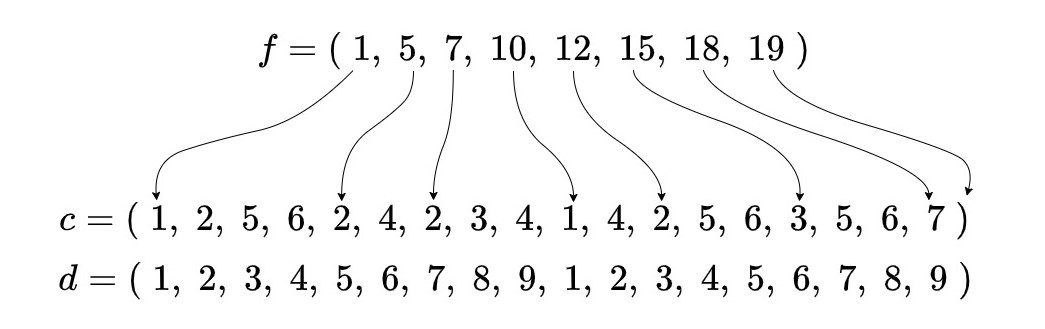
\includegraphics[width=\textwidth]{imagenes/chapter2/csr-format.jpg}
\end{center}
\caption{Matriz $A$ almacenada en formato CRS.}
\label{crs-matrix}
\end{figure}


En la Figura~\ref{crs-matrix} se muestra cómo se representa la matriz $A$ utilizando la estrategia CRS.
Para acceder al valor $A(i,j)$ de la matriz $A$, se obtienen primero los \'indices $p_1=f(i)$ y $p_2=f(i+1)$, posteriormente se busca el \'indice $p$ tal que $p_1 \leq p < p_2$ y $c(p) = j$, y luego se puede obtener el valor buscado accediendo a $d(p)$. 
 
 Si la matriz tiene más coeficientes no nulos que cantidad de filas, la estrategia CRS utiliza menos memoria que el formato simple. Es necesario conocer todas las posiciones de los coeficientes para generar la estructura en forma eficiente o, dicho de otra forma, es muy difícil agregar un nuevo valor a la estructura, a menos que sean posteriores en la matriz al último elemento ya presente. Este formato permite acceder fácilmente a todos los elementos de una fila, pero no a los de una columna.


\subsection{CCS (Compressed Column Storage)}

 El formato comprimido por columna es similar al CRS pero utilizando el vector comprimido para las columnas.
En la Figura~\ref{ccs-matrix} se muestra como se aplica esta estrategia a la matriz $A$.

\begin{figure}[h]
\begin{center}
\begin{eqnarray*}
d = \left(
\begin{array}{cccccccccccccccccc}
1 & 1 & 2 & 5 & 7 & 3 & 8 & 6 & 6 & 9 & 2 & 3 & 4 & 7 & 4 & 5 & 8 & 9\\
\end{array}
\right)\nonumber\\
f = \left(
\begin{array}{cccccccccccccccccc}
1 & 4 & 1 & 2 & 3 & 5 & 3 & 6 & 2 & 3 & 4 & 1 & 5 & 6 & 1 & 5 & 6 & 7\\
\end{array}
\right)\\
c = \left(
\begin{array}{cccccccc}
1 & 3 & 7 & 9 & 12 & 15 & 18 & 19\\
\end{array}
\right)\nonumber
\end{eqnarray*}
\end{center}
\caption{Matriz A almacenada en formato CCS.}
\label{ccs-matrix}
\end{figure}

 Se mantienen las necesidades de memoria del formato CRS y en cuanto a las características de acceso se invierten los conceptos con respecto  a filas y columnas.
 
\subsection{DIA (DIAgonal format)}\label{dia-format}

 \begin{figure}[h]
     \centering
     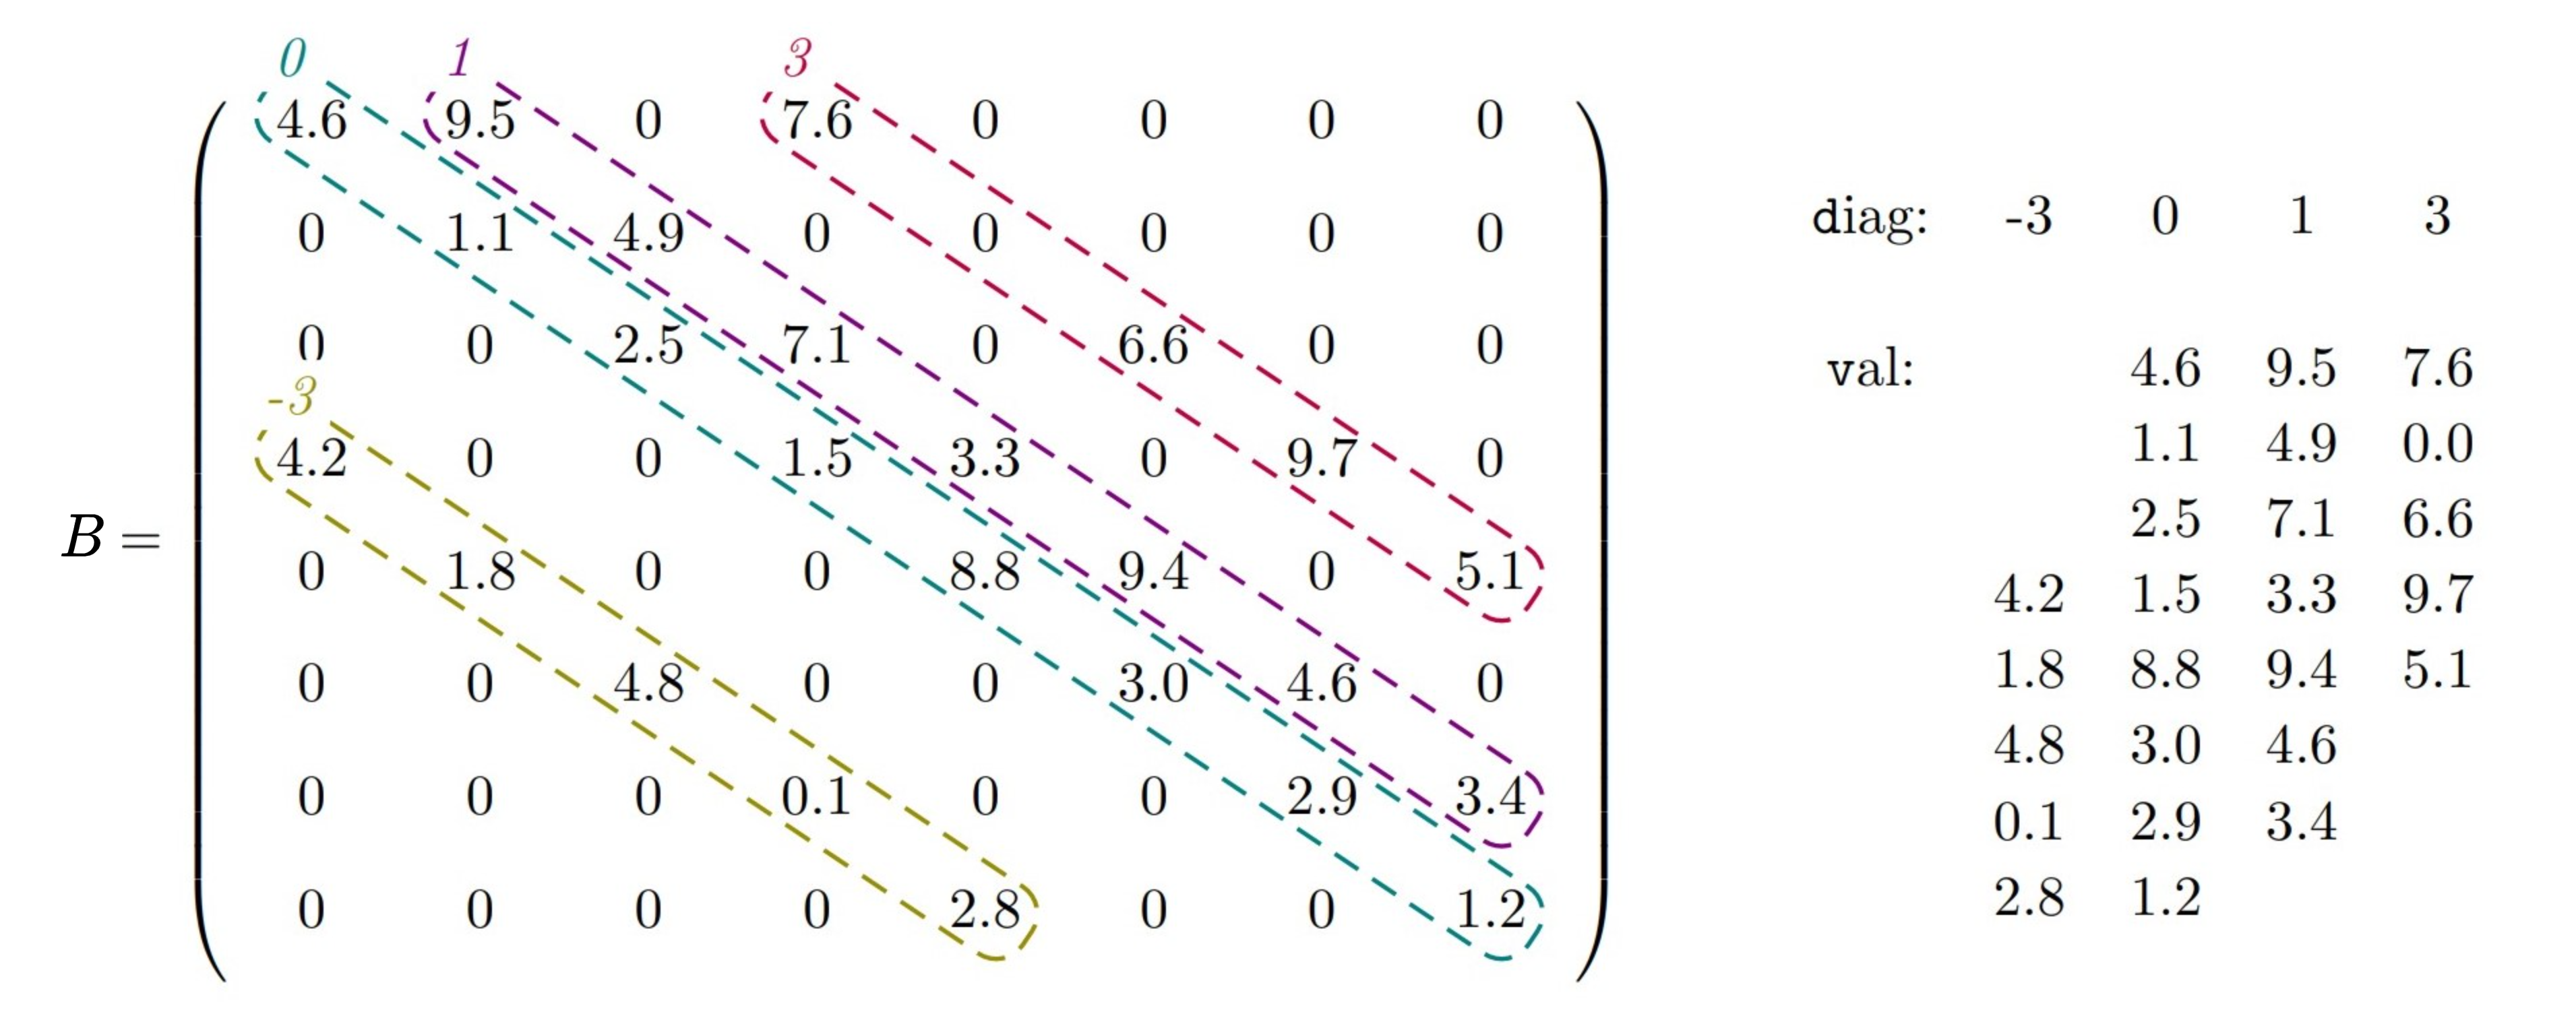
\includegraphics[width=\textwidth]{imagenes/chapter2/diag-format-B.png}
     \caption{Matriz $B$ almacenada en formato DIA.}
     \label{fig:diag-format}
 \end{figure}
 
 
 Cuando la matriz a almacenar es de banda, se pueden utilizar estrategias de almacenamiento por diagonales.
Entonces se almacena la matriz original en una matriz rectangular de tamaño  $n \times d$ siendo $n$ la dimensión de la matriz y $d$ la cantidad de diagonales.


 Si se desea almacenar una matriz que posee $d$ diagonales no consecutivas, % en las que se encuentran los coeficientes distintos de cero pero no siendo las diagonales principales
 una variante de formato es el \textit{DIAgonal storage Format}  que  utiliza una matriz de tamaño $n\times d$ en la que se almacenan las $d$ diagonales y un vector de tamaño $d$ en el que se  especifica el desplazamiento de cada diagonal con la diagonal principal, estando la diagonal principal asociada con 0, las diagonales ``por encima'' con valores positivos y ``por debajo'' con valores negativos. En la Figura~\ref{fig:diag-format} se puede ver un ejemplo.
 


\subsection{ELL (Ellpack-itpack)}\label{ell-format}


En el formato \textit{Ellpack-itpack}, se utiliza una estructura densa de tamaño $n\times k$, donde $n$ es la cantidad de filas y $k = max_i(\nnz(A_i))$, con $A_i$ la fila $i$-ésima de la matriz, es decir, la cantidad máxima de elementos no nulos por fila. La matriz dispersa es almacenada en dos matrices ``densas'' de tamaño $n\times k$, una con las entradas no nulas de la matriz y otra con los índices de las columnas. Es necesario agregar explícitamente valores nulos para completar la primer matriz (\textit{zero padding}). Este problema es menor cuando todas las filas de la matriz son de largos similares (el caso ideal son las matrices con cantidad constante de elementos por fila/columna). En la Figura~\ref{fig:ell-matrix}, se puede observar como se almacena una matriz en formato ELL.

Dado que la estructura elegida es de tamaño $n \times k$, es decir, tiene la misma cantidad de filas que la matriz original, no es necesario almacenar explícitamente los índices de fila ya que están implícitos en la estructura, a diferencia de otros formatos, como por ejemplo COO.

% TRABAJANDO EN IMAGENES MEJORES

% EL PORQUE DEL HYB (hybrid format propuesto por  Bell and Garland)
% Este formato es poco eficiente cuando la cantidad de elementos no nulos en cada fila varia considerablemente respecto al promedio de elementos no nulos por fila. Dado el caso, hay una pérdida en términos del espacio necesario para almacenar la matriz, asi como 
% \begin{figure}
%     \centering
%     \begin{eqnarray*}
%     \left(
%     \begin{array}{ccccccc} 
%     1 & 2 & 3 & 4 \\
%     5 & 6 & 0 & 0 & 0\\
%     7 & 8 & 9 & 0 & 0 & 0\\
%     1 & 2 & 0 & 0 & 0\\
%     3 & 4 & 5 & 0 & 0\\
%     6 & 7 & 8 & 0 & 0 & 0\\
%     9 & 0 & 0 \\
%     \end{array}
%     \right)
%     \end{eqnarray*}
%     \caption{Matriz $A$ en el formato ELL (INCOMPLETO).}
%     \label{fig:ell-matrix}
% \end{figure}

\begin{figure}
    \centering
    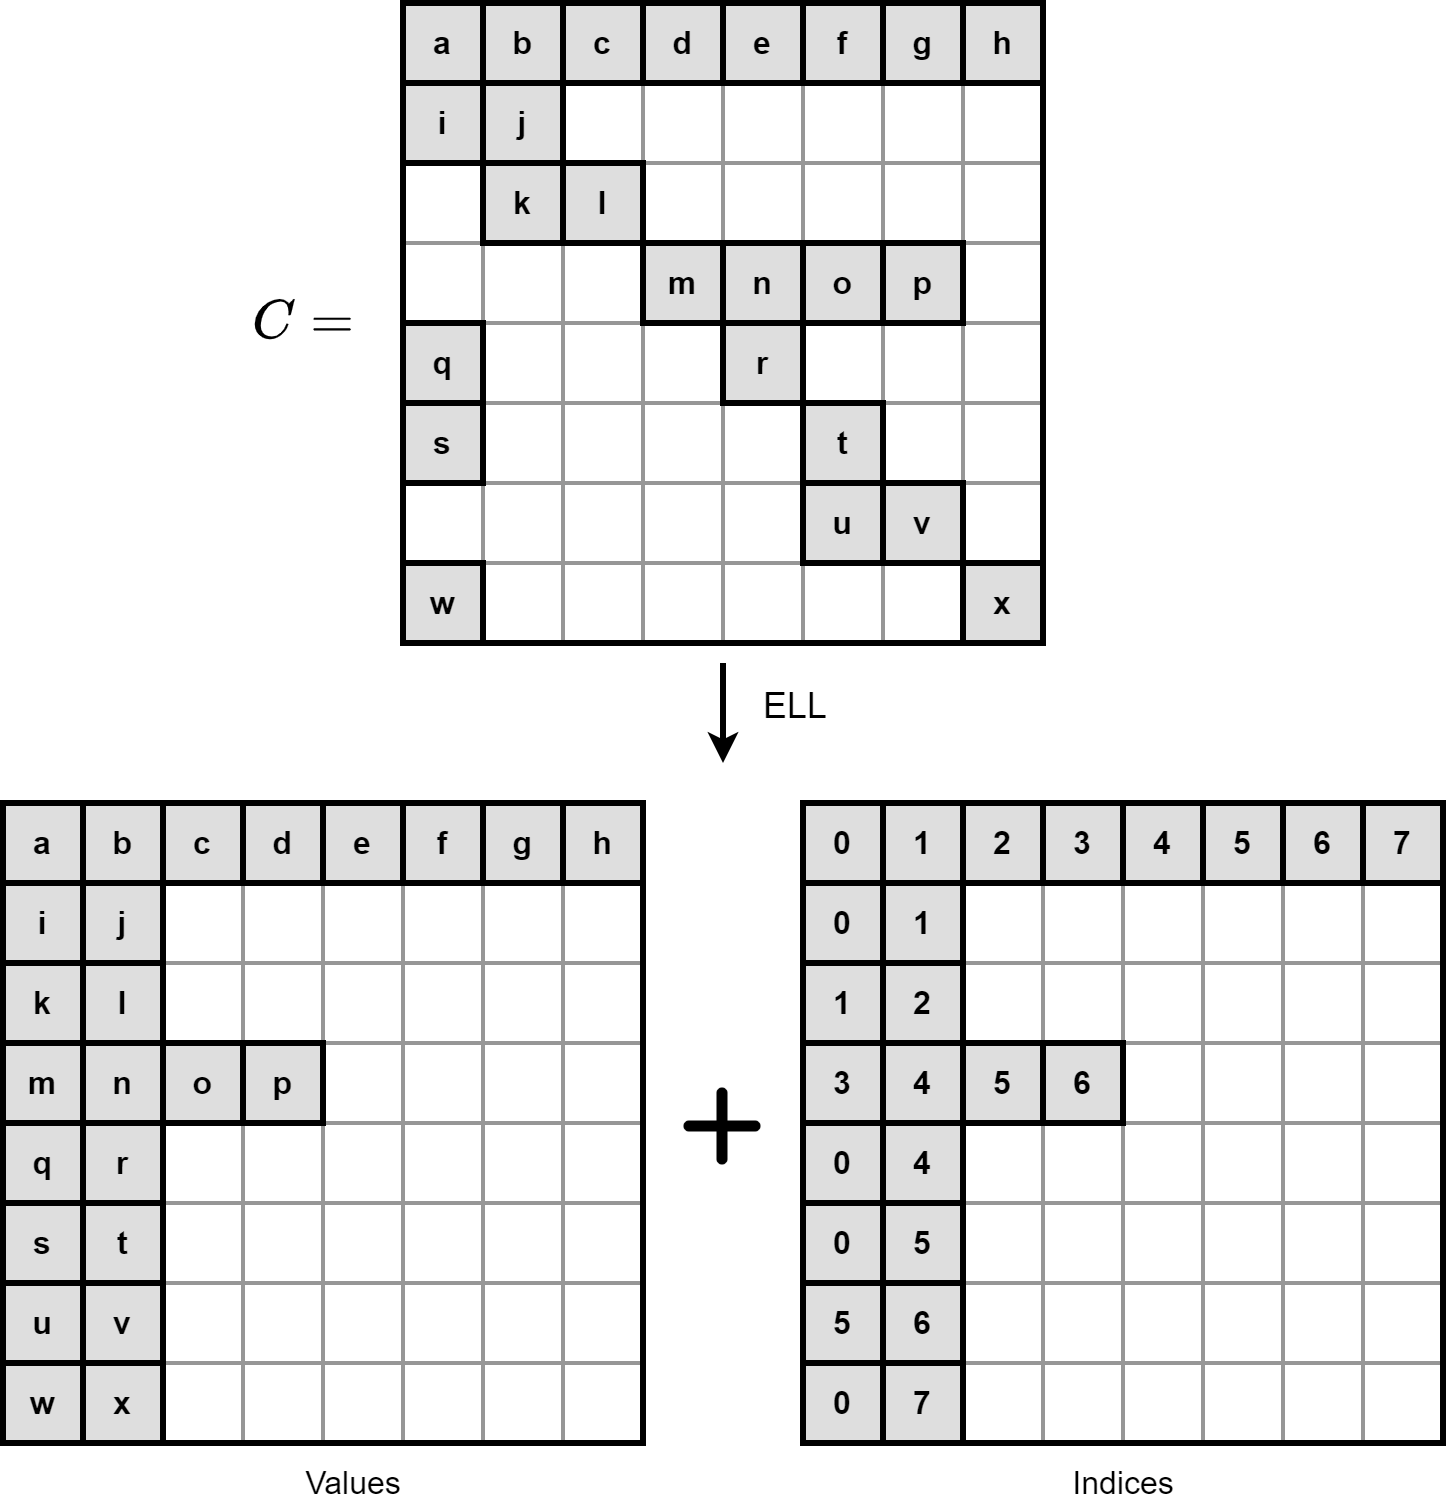
\includegraphics[width=0.7\textwidth]{imagenes/chapter2/ell.png}
    \caption{Matriz $C$ almacenada en formato ELL.}
    \label{fig:ell-matrix}
\end{figure}


\subsection{BCRS (Block Compressed Row Storage)}\label{bcrs}

\begin{figure}
    \centering
    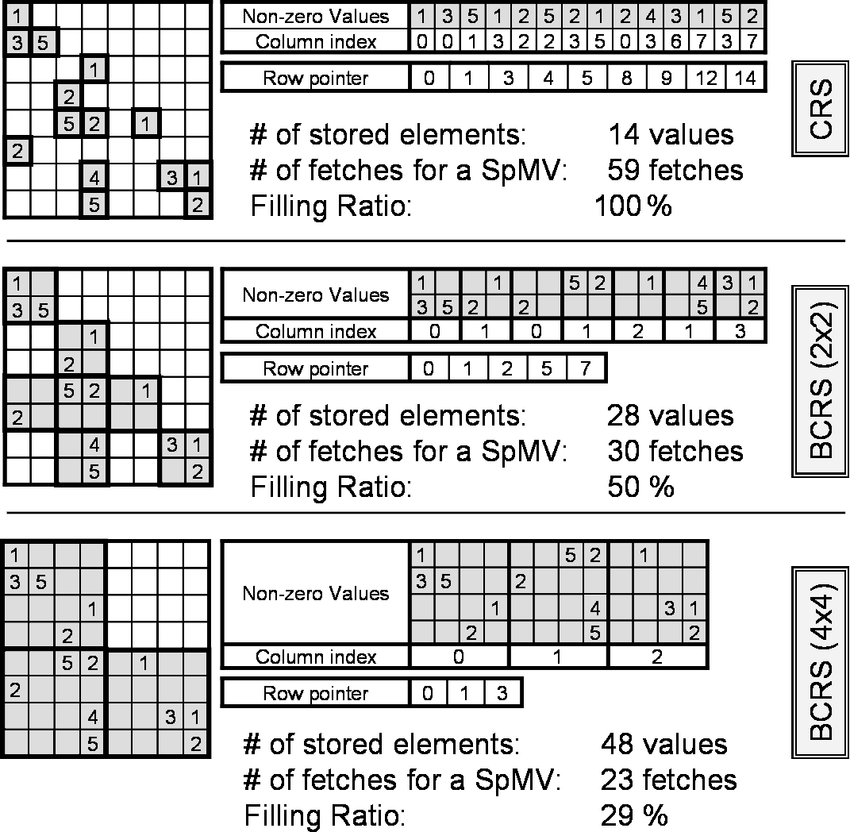
\includegraphics[width=\textwidth]{imagenes/chapter2/bcrs.png}
    \caption{Ejemplo de matriz almacenada en formato BCRS aplicado con distintos tamaños de bloque y comparación con CRS. Extraído de \cite{Buatois2009}.}
    \label{fig:bcrs}
\end{figure}

Este formato se utiliza cuando la matriz se puede dividir/almacenar eficientemente como sub-bloques regulares.

Se tiene entonces, una matriz de $n \times m$ con $nnz_b$ bloques de dimensión $n_b$\footnote{En general los bloques son cuadrados y tanto $m$ como $n$ son múltiplos de $n_b$.}, con entradas de números en punto flotante, enfocada a almacenar los elementos no nulos, además de dos vectores de números enteros, uno para el índice de columna de cada sub-bloque y el otro con el índice (puntero) al comienzo de cada fila.

Notar que este formato funciona razonablemente bien si la matriz posee bloques regulares.

\subsection{BCCS (Block Compressed Column Storage)}\label{bccs}

Funciona de la misma manera que BCRS pero, a la hora de acceder a cada sub-bloque de la matriz, se utiliza CCS.

%\subsubsection{JDS}
%\subsubsection{SKS}



% \subsection{Estrategias Dinámicas}
% %  Las distintas estrategias din\'amicas generalmente utilizan punteros para implementar las estructuras, por lo tanto para implementar las  variantes es necesario utilizar lenguajes que soporten \texttt{allocate} din'amico por ejemplo \texttt{C} y \texttt{Fortran 90}.
% Este tipo de formatos no son de uso común en el álgebra lineal numérica, al menos en las últimas décadas, y su uso es más difundido en campos como las bases de datos. Se incluyen en la revisión por completitud. 
\subsection{LLRCS (Linked List Row-Column Storage)}

En esta estrategia se utiliza una multi-estructura bidimensional. 
Cada entrada correspondiente a un no-nulo contiene dos punteros a sus adyacentes por
fila, y dos a sus adyacentes por columna. Además, dispone de dos vectores de tamaño igual a la cantidad de filas y columnas,  
% en cada entrada se dispone de un puntero para recorrer  las distintas entradas por fila en un vector o por columna en el otro.
con punteros al comienzo de cada fila o columna, respectivamente.

La memoria que se necesita para implementar la estrategia LLRCS, si \nnz es la cantidad de coeficientes no nulos,  se necesitan \nnz posiciones de  punto flotante, $4\ \times\ $\nnz punteros, \nnz enteros, más la memoria necesaria para almacenar los dos vectores ($2 \times n$ punteros).

 Para acceder al valor $A(i,j)$ se puede recorrer la lista de la entrada $i$ por el vector de filas buscando el valor cuya columna sea $j$, o recorrer la lista de la entrada $j$ del vector de columnas hasta encontrar la fila $i$. 
%\pagebreak

\subsection{LLRS (Linked List Row Storage)}

 En esta estrategia se utiliza una estructura unidimensional, en la cual se emplea un vector de tamaño igual a la cantidad de filas, y de cada posición del vector se puede obtener la lista de entradas de esa fila.
 
 En cuanto a memoria, se necesitan \nnz posiciones de punto flotante, \nnz enteros, \nnz  punteros, más el vector de entrada ($n$ punteros). 


\subsection{LLCS (Linked List Column Storage)}

Al igual que en la propuesta anterior, en la estrategia LLCS se utiliza una estructura unidimensional, pero el vector base de la estructura es de tamaño igual a la cantidad de columnas y de cada posición del vector se puede obtener la lista de coeficientes no nulos de esa columna. La estrategia LLCS posee las mismas necesidades de memoria que la LLRS.



\section{Multiplicación Matriz-Vector (SpMV)}\label{spmv}

Si bien el objetivo del proyecto no se centra en estudiar las matrices dispersas para una operación particular, la importancia que implica la operatoria al trabajar con éstas obliga a mostrar algunas operaciones específicas. Por esta razón, en este apartado se presenta la multiplicación Matriz Dispersa-Vector (SpMV por su nombre en Inglés Sparse Matrix-Vector). La SpMV \cite{golub1996matrix} es una operación de la forma $y = Ax$, donde $A$ es una matriz dispersa de tamaño $m\times n$, los vectores $x$ e $y$ son densos de tamaño $n$ y $m$ respectivamente. Este kernel es altamente utilizado y con enormes aplicaciones en la computación científica. Dada su importancia, la implementación de esta operación ha sido fuertemente estudiada  en variedad de contextos, desde diferentes formatos dispersos, hasta diversas arquitecturas de hardware, entre ellas: GPUs, FPGAs e incluso en dispositivos como TPUs~\cite{Ku2008,Reguly2012,He2020}. %Si bien la carga computacional de esta operación no es elevada, debido a que la matriz es dispersa y la multiplicación por los coeficientes nulos no es necesaria computarla, 

Si bien las operaciones necesarias para su cómputo son simples (sumas y multiplicaciones), la SpMV, presenta ciertas limitantes a la hora de su ejecución.
El cuello de botella se da en los accesos a memoria (principalmente por la aleatoriedad de los accesos). 
Este hecho ha motivado que muchos esfuerzos por optimizar la SpMV se centren en definir formatos de almacenamiento adecuados. Esto ha permitido que en muchas de las implementaciones de la operación SpMV, los accesos a la matriz $A$ sean ordenados y bien aprovechados, obteniendo accesos predecibles y eficientes. Mientras que, en general, el vector $x$ es accedido de forma irregular debido a la estructura de la matriz $A$, sacando poco beneficio de la localidad de datos y desaprovechando del uso de memorias cache. %(Posibles planteos para mejorar dichos accesos :reducir el ancho de banda de la matriz, dando accesos mucho mas coalesced, estrategia a evaluar en el correr del proy. aplicando por ejemplo RCM)

A modo de ejemplo, en el Algoritmo~\ref{alg:CSR_serial}, se presenta en alto nivel el procedimiento secuencial que computa SpMV, utilizando el formato CSR para almacenar la matriz $A$. El primer ciclo \texttt{for} ($i$) recorre las filas de la matriz $A$, y el segundo \texttt{for} interno ($j$) calcula, accediendo a los elementos no nulos almacenados en $d$ a través de los punteros en $f$, para cada fila, la multiplicación por los coeficientes correspondientes del vector~$x$ (accedido en las posiciones donde existen elementos no nulos indicado por $c$) y se almacena el resultado en la posición del vector~$y$ pertinente.

\begin{algorithm}[th]
\textbf{Input:} $f, c, d, x$ \\
\textbf{Output:} $y$
\begin{algorithmic}
\STATE{$y = 0$}
%\STATE{in parallel...}
\FOR{$i = 1$ \TO $m$}
\FOR{$j = f[i]$ \TO $f[i+1]-1$ }
\STATE{$y[i] = y[i] + d[j] \cdot x[c[j]]$}
\ENDFOR
\ENDFOR
\end{algorithmic}
\caption{
% Serial computation of sparse matrix-vector multiplication (SpMV) with the sparse matrix $A$ stored in the CSR format.
% The vector $d$ stores the nonzero values of $A$ by rows;  $f$ contains the indexes that specify the first element %correspond to the beginning
% of each row in vector $d$; and $c$ contains the column index of each element in the original matrix.
% The nonzero elements within each row are ordered by column index.
% %Typical procedure of the \spmv for the CSR sparse storage format.
Cálculo secuencial de la multiplicación matriz dispersa-vector (SpMV) con la matriz dispersa $A$ almacenada en el formato CSR. 
El vector $d$ almacena los valores distintos de cero de A por filas, $f$ contiene los índices que especifican el primer elemento de cada fila en el vector $d$; y $c$ contiene el índice de columna de cada elemento en la matriz original. 
Los elementos distintos de cero dentro de cada fila están ordenados por índice de columna.
}
\label{alg:CSR_serial}
\end{algorithm}


\section{Estrategias de reordenamiento}\label{sec:reordenamientos}

% \resumen{Por que reordenar}

Como se menciona en las secciones anteriores, muchas de las matrices dispersas con las que se trabaja en la actualidad corresponden a discretizaciones de problemas de redes eléctricas y distribución de energía, ingeniería estructural, etc. y, más en general, formulaciones de sistemas de ecuaciones diferenciales parciales. Estos sistemas son aproximados mediante ecuaciones con una cantidad finita de incógnitas, y resultan en sistemas de la forma $Ax = b$, con $A$ una matriz dispersa.
Buscando explotar estas características, por muchos años, la estrategia más difundida fue intentar llevar las matrices a una matriz equivalente pero de banda. Notar que, una matriz con un ancho de banda pequeño es útil principalmente por dos razones. La primera es que permite utilizar una estructura de datos simple en métodos directos como la factorización LU para resolver sistemas lineales dispersos. Segundo, también es útil en métodos iterativos como el método del Gradiente Conjugado, porque los elementos distintos de cero serán agrupados cerca de la diagonal, mejorando así la localidad de los datos. 

%\resumen{Que es reordenar}

En este contexto se desarrollaron las técnicas de reordemaniento para las matrices dispersas. Reordenar es encontrar una permutación $p$ que se aplica tanto para filas como para las columnas de la matriz. Este reordenamiento puede buscar diferentes objetivos. Dada una matriz simétrica $A$, un reordenamiento de reducción de ancho de banda apunta a encontrar una permutación $P$ de modo que el ancho de banda de $PAP^t$ sea pequeño (en el ideal, mínimo). 

Notar que en los problemas que provienen de estructuras de grilla, reordenar la matriz es equivalente a renumerar los nodos de la grilla. Este aspecto también ha sido especialmente abordado en dicho campo de estudio (la generación de grillas de discretización).


%\resumen{el por que de las heurísticas, definir heurística???}

Dado que el problema de encontrar el reordenamiento que minimice el ancho de banda para una matriz es un problema $\mathcal{NP}$-completo~\cite{Papadimitriou1976}, se ha trabajado en estudiar e implementar múltiples heurísticas con el objetivo de encontrar buenas soluciones con esfuerzos computacionales razonables. Una familia importante de estos algoritmos, trata la reducción del ancho de banda de una matriz, como se dijo antes, bajo la perspectiva de un problema de etiquetado de grafos. De esta manera, el problema de reordenar una matriz dispersa $A$ equivale al de etiquetar los vértices o nodos del grafo correspondiente a interpretar $A$ como la matriz de adyacencia asociada. Esto es interpretar cada fila o columna $i$ como un nodo de un grafo, y cada entrada no nula $j$ de dicha fila como una arista que conecta el nodo $i$ con el $j$, tal como muestra la Figura~\ref{fig:adjacency-matrix}. %(SEGURO SE PUEDE REDACTAR MRJOT O ESCRIBIR EN LENGUAJE MAS MATEMATICO con G(V,E) V = 1..n y E = (i,j) tal que $a_ij$ disitnto de 0, que me recomendas?)

\begin{figure}
    \centering
    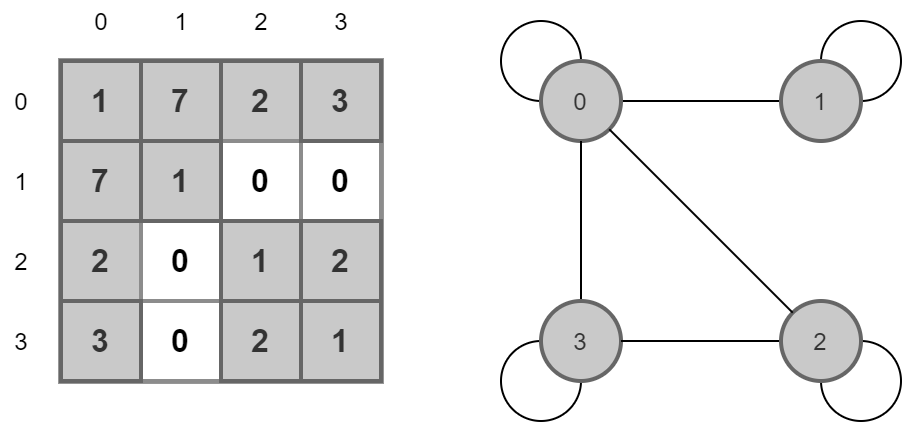
\includegraphics[width=0.6\textwidth]{imagenes/chapter2/adjacency-matrix.png}
    \caption{Ejemplo de grafo y su matriz de adyacencia correspondiente.}
    \label{fig:adjacency-matrix}
\end{figure}  

% 1. Una de las razones por las cuales se aplican estrategias de reordenamiento sobre las filas y columnas de una matriz, es para reducir la cantidad de \textit{fill-in} (DEFINIR EN ALGUN LADO) que crea la factorización, reduciendo así el tiempo y el costo de almacenamiento de los cálculos posteriores.
% 2. Otra de las razones para reordenar matrices dispersas es para reducir los accesos a memoria en durante SpMV. Aplicando re-ordenamientos que reduzcan el ancho de banda (RCM GPS), permite en algunos casos poder almacenar dicha matriz en un formato que aproveche estas características (DIA).


A continuación, son presentadas las heurísticas clásicas para la reducción del ancho de banda, Cuthill-McKee (CM)~\cite{Cuthill-Mckee}, Reverse Cuthill-McKee (RCM)~\cite{alan-phdthesis} y Gibbs-Poole-Stockmeyer (GPS)~\cite{Gibbs1976}. Es preciso mencionar que, a pesar que estas herramientas funcionan relativamente bien, no hay que dejar de lado que son  heurísticas, por lo tanto no son métodos que garanticen alcanzar la solución óptima, sino que una solución aceptable buscando un buen balance costo/beneficio.

 \subsection{Cuthill-McKee (CM)}\label{CM}

El algoritmo de Cuthill-McKee~\cite{Cuthill-Mckee}, está basado en la aplicación de una estrategia de recorrida Breadth-First-Search (BFS), en la que el grafo asociado a la matriz es atravesado por niveles, determinados a partir del nodo raíz (nivel 0). A medida que se atraviesan los nodos de un nivel, a estos se los marca y numera en base al orden en que son recorridos. A continuación, se inspeccionan los vecinos de cada uno de estos nodos marcados, cada vez que se encuentra un vecino de un nodo visitado que no está numerado, se lo agrega a una lista y se etiqueta como el siguiente elemento del siguiente nivel. El orden en el que se atraviesa cada nivel da lugar a diferentes ordenamientos o permutaciones de filas y columnas. En el proceso de reordenar, en el algoritmo Cuthill-McKee, los nodos adyacentes a un nodo visitado siempre se atraviesan del grado más bajo al más alto.


\begin{algorithm}[]
%\SetAlgoLined
\textbf{Input:} Grafo $G$ \\
\textbf{Output:} $p$



 $v_1 \leftarrow r$; // Nodo inicial o raíz, en algunos casos el de menor grado - nodo periférico  \
 
 \For{$i = 1$ \KwTo $n$}{
  Encontrar todos los nodos adyacentes de $v_i$ sin numerar\; %Find all the unnumbered neighbors of the vertex $v_i$\;
  Etiquetar los nodos encontrados en orden creciente de grado\; %Label the vertices found in increasing order of degree\;
%   \eIf{condition}{
   
%   }{
%   instructions3\;
%   }
 }
 \caption{Cuthill-McKee. Esquema general en alto nivel del algoritmo Cuthill-McKee.}
 \label{alg:cm}
\end{algorithm}

\subsection{Reverse Cuthill-McKee (RCM)}\label{RCM}
Variante del algoritmo CM, anteriormente descrito, en el que se ``invierte'' el orden obtenido para las filas/columnas.
La heurística RCM produce como resultado matrices con el mismo ancho de banda que CM, pero con \textit{profile} menor.

En la versión original de la heurística RCM propuesta por Alan George, también son seleccionados como vértices iniciales aquellos con grado mínimo en el grafo y se generan las estructuras de nivel desde estos vértices.

Las reducciones de ancho de banda y profile de la matriz resultante, obtenidas por las heurísticas CM y RCM, dependen fuertemente de la elección del vértice inicial. Por esto se han realizado varios estudios de como elegir el vértice inicial de manera de lograr optimizaciones en el proceso de encontrar ordenamientos aceptables.


\subsection{Gibbs-Poole-Stockmeyer (GPS)}

Antes de profundizar en esta heurística, es importante presentar algunas definiciones básicas útiles para la técnica, en especial considerando que los autores utilizan el concepto del grafo asociado a la matriz dispersa.

Definición (\textit{distancia}). La distancia, función definida para dos vértices del grafo $\mathit{d} : V \times V \longrightarrow \mathbb{N}$. Sean $u$ y $v$ vértices, la distancia $\mathit{d}(u,v)$ está dada por el largo del camino mínimo entre éstos.

Definición (\textit{excentricidad}). La excentricidad, definida sobre un vértice del grafo, $\mathit{l} : V \longrightarrow \mathbb{N}$, está dada por $\mathit{l}(v) = max_{v,u \in V}(d(v,u))$.

Definición (\textit{diámetro del grafo}). El diámetro $\Phi(G) = max_{v \in V} (\mathit{l}(v)) = max_{v,u \in V} (d(u,v)) $ del grafo $G(V,E)$ es la mayor excentricidad presente en G.


Gibs, Poole y Stockmeyer posteriormente del surgimiento de las heurísticas CM y RCM, verificaron que éstas heurísticas no eran adecuadas en los casos que la elección del vértice inicial implica un costo computacional grande. En dichas técnicas los vértices iniciales son los de menor grado en el grafo, y luego se generan las estructuras de nivel a partir de éstos. Notar, por ejemplo, que CM y RCM harían un cómputo innecesario en situaciones donde los vértices tienen todos el mismo grado. 

Para comprender el algoritmo GPS, es necesario dar   una definición de nodo o vértice pseudo-periférico:

Definición (\textit{vértice periférico}). Un vértice $v$ es considerado periférico si su excentricidad es igual al diámetro del grafo, i.e.  $\mathbf{l}(v) = \Phi(G)$.
Entonces, para Gibbs, Poole y Stockmeyer, un vértice es pseudo-periférico si su excentricidad es cercana al diámetro del grafo. 

En GPS, en lugar de construir varias estructuras de nivel, como en las planteadas en CM y RCM,  sólo se construyen dos (con nodos raíces dos vértices pseudoperiféricos). Gibbs, Poole y Stockmeyer, fueron los primeros autores en utilizar un vértice pseudo-periférico como inicial para la renumeración. Las bondades que ofrece elegir un vértice pseudo-periférico como vértice inicial para renumerar se dan debido a que en la estructura de nivel formada desde este vértice habrá mayor cantidad de niveles y, en consecuencia, menos ancho por nivel, comparado con un vértice que no está en la periferia o cerca de la periferia del grafo de adyacencia.

La heurística GPS se puede dividir principalmente en tres etapas. 
En el primer paso de la heurística GPS, se seleccionan dos nodos pseudo-periféricos, $v, u \in V$, y sus estructuras de nivel asociadas $\mathit{L}(v)$ y $\mathit{L}(u)$, respectivamente, tomando a estos como raíz.
En la segunda etapa de la heurística GPS, en base a las estructuras anteriormente mencionadas en la etapa uno, $L(v)$ y $L(u)$, se crea una nueva estructura de nivel, $K(v, ...)$. Se combina las estructuras de nivel con el objetivo de reducir el ancho por nivel (que sería equivalente al ancho de banda). Este paso asegura que el ancho de nivel de la estructura $K (v, ...)$ sea, como máximo, el ancho de nivel más pequeño de las estructuras de nivel $\mathit{L}(v)$ y $\mathit{L}(u)$.
Finalmente, en el último paso, se renumeran los vértices atravesando la estructura del nivel $K(v, ···)$ generada en la segunda etapa de la heurística GPS. Los niveles se recorren en orden inverso, es decir, desde el nivel $K_{l(v)}(v, ...)$ hasta el nivel $K_{0}(v, ...)$. Esta renumeración se realiza nivel a nivel de la estructura generada, en la que la renumeración de los vértices se realiza en orden ascendente de grado. 



\subsection{Algoritmo Sloan (Sloan)}

%\resumen{El Algoritmo Sloan utiliza pesos, con los que calcula una cierta prioridad entre los nodos, me pareció interesante la técnica}

El algoritmo Sloan~\cite{Sloan1986} es una heurística planteada por Scott W. Sloan en el año 1986 para reordenar matrices dispersas. Normalmente, se utiliza para acelerar el cálculo de sistemas de ecuaciones lineales dispersos como muchas de las otras heurísticas de reordenamientos. 

La idea principal del algoritmo es numerar los vértices desde un punto cercano al diámetro del grafo, un pseudo-diámetro%, manteniendo (en la medida de lo posible) este valor a través del ordenamiento
. En el primer paso, se busca un pseudo-diámetro del grafo y se eligen $s$ y $e$ como extremos de dicho camino. En el paso dos, a cada vértice del grafo se le asocia una cierta prioridad, en base al pseudo-diámetro anterior y al grado de éste, inmediatamente, el vértice inicial $s$ se ordena primero. Luego, en cada etapa, se elige el siguiente vértice a numerar entre el conjunto factible con la mayor prioridad. Manteniendo así, un equilibrio entre los objetivos de mantener un \textit{profile} pequeño y la incorporación de vértices elegibles que se han quedado atrás (lejos de $e$). La lista de vértices posibles para numerar en cada iteración, está formada por los vecinos de uno o más vértices ya renumerados y los vecinos de estos.
 
 El algoritmo, puede entonces, dividirse principalmente en dos fases bien distintivas: (1) selección del vértice inicial $s$ y final $e$, y (2) reordenamiento de vértices.% A esta altura, es clara la importancia de la elección de los vértices iniciales, etapa a la que se le da prioridad en los diferentes algoritmos de reordenamiento. Continuando con el algoritmo,  

Para la prioridad de cada nodo, se utilizan dos pesos positivos $W_1$ y $W_2$ de forma de ponderar las dos propiedades que determinan la prioridad del nodo, en este caso son la distancia al nodo inicial y el grado, respectivamente. 
$P(n) = W_1\times distance(n,s) - W_2\times degree(n)$.

\begin{algorithm}[]
\textbf{Input:} Grafo $G$, Pesos $W_1, W_2$, Nodos $s,e$ \\
\textbf{Output:} $p$
\begin{algorithmic}
% \COMMENT{Inicializar los vertices}
\STATE nextId = 0;
\FOR{\textbf{each} $n$ Node \textbf{in} G}
\STATE{status(n) = inactive;}
\STATE priority(n) = $W_1 \times$ distance(n,s) - $W_2 \times$ degree(n);
\ENDFOR

\STATE status(s) = preactive;
\STATE working\_queue = \{s\};

\FOR{\textbf{each} $n$ node \textbf{in} working\_queue \textbf{order by} priority}
\FOR{\textbf{each} $v$ \textbf{in} Neighbors($n$)}
\IF{status(n) == preactive \AND (status(v) == inactive \OR status(v) == preactive))}
    \STATE update(priority(v));
    \STATE status(v) = preactive;
    \STATE updateFarNeighbors(v,working\_queue);
\ELSIF{status(n) == preactive \AND status(v) == active)}
    \STATE update(priority(v));
\ELSIF{ status(n) == active  status(v) == preactive)}
    \STATE update(priority(v));
    \STATE status(v) = active;
    \STATE updateFarNeighbors(v,working\_queue);
\ENDIF
\STATE p[nextId++] = n;
\STATE status(n) = numbered;
\ENDFOR
\ENDFOR

\FOR{$i = 1$ \TO $m$}
\FOR{$j = f[i]$ \TO $f[i+1]-1$ }
\STATE{$y[i] = y[i] + d[j] \cdot x[c[j]]$}
\ENDFOR
\ENDFOR
\end{algorithmic}
\caption{
Algoritmo Sloan. Pseudocódigo para una posible implementación secuencial del algoritmo Sloan. Extraído de~\cite{sloan-parallel}.
}
\label{alg:sloan-serial}
\end{algorithm}

El Algoritmo~\ref{alg:sloan-serial} presenta un pseudocódigo de cómo funciona el algoritmo Sloan. En cada iteración, los  nodos del grafo puede estar en uno de 4 estados: (i) \textit{numerado}, (ii) \textit{activo}, (iii) \textit{preactivo}, para los nodos vecinos de algún nodo activo, y un cuarto estado (iv) \textit{inactivo} para el resto de los nodos. Inicialmente, sólo el nodo inicial $s$ está en estado \textit{preactivo} mientras que el resto se encuentra en estado \textit{inactivo}. Seguido, el algoritmo itera a través de todos los nodos del grafo, y en cada paso elige entre los nodos \textit{activos} o \textit{preactivos} en orden descendente de prioridad, es decir, maximizando en cada paso la prioridad. Posteriormente, se asignan nuevas prioridades a los vecinos y los vecinos de éstos son seleccionados para procesar.

Existen también, implementaciones en paralelo para este algoritmo, tal y como se  plantea en~\cite{sloan-parallel}.

%(Pueden haber otros ordenamientos, que no busquen reducir el ancho de banda, sino el fill in producido a la hora de operar, por ejemplo en métodos iterativos x exactos ???). Parrafo diciendo que tambien se usa para otras cosas.....


\newpage\section{Plataformas de hardware heterogéneas en HPC}

% \resumen{intro feneral para arquitect de hpc}

La computación de alta performance (HPC), al día de hoy, es una de las herramientas más importantes para el avance de la computación científica. 
El desarrollo tecnológico ha motivado resolver problemas más grandes y/o con mayor precisión. Esto, a su vez, se retro-alimenta y genera aún mayores necesidades computacionales. En este contexto, la HPC aporta en soluciones tecnológicas que sirven de base para abordar este tipo de realidades. Entre otros campos, el uso de HPC ha permitido el desarrollo de áreas %Como se ha mencionado anteriormente, así como las matrices dispersas modelan tantos problemas científicos complejos, con las arquitecturas y el hardware enfocado al HPC, se buscan resolver, 
como el pronóstico del tiempo, la exploración de energía, la bioinformática~\cite{hpc-bioinformatics}, el % hasta la dinámica de fluidos computacional, combinar simulaciones tradicionales con inteligencia artificial, 
aprendizaje automático, el análisis de big data~\cite{big-data2015} y el edge-computing~\cite{Tu2019}.


Entre las arquitecturas de hardware utilizadas para la HPC se encuentran las unidades de procesamiento gráfico, o GPU (del inglés Graphics Processing Units). Son coprocesadores diseñados originalmente para alivianar la carga de la CPU en aplicaciones con una importante carga de trabajo dedicada a la representación de gráficos en la pantalla, como pueden ser videojuegos o simulaciones con un alto contenido de imágenes 3D, entre otras cosas~\cite{Kirk2013}. 
En los últimos años, los avances tanto en el hardware como en distintos lenguajes de programación orientados a estas arquitecturas, que permiten, no sólo trabajar con procesamiento gráfico, sino que también con problemas de propósito general como simulaciones y modelos numéricos. Entre los lenguajes orientados a este tipo de arquitecturas se destaca \texttt{CUDA} (estándar de bibliotecas de la empresa \texttt{Nvidia}). Gracias a la programabilidad y flexibilidad de la arquitectura \texttt{CUDA}, las GPU han pasado a ser verdaderos procesadores masivamente paralelos, presentes en la mayoría de las plataformas de HPC modernas.
Debido a la gran importancia que han tenido las GPUs en la computación científica, y en particular en el ALN, se dedica la Sección~\ref{sec:gpu-arch} al estudio de su arquitectura.
% Este desarrollo transforma a las GPUs en verdaderos procesadores masivamente paralelos, ofreciendo altos niveles de cómputo.



\subsection{Arquitectura de las GPUs}\label{sec:gpu-arch}
% Es normal comparar el rendimiento de las GPUs frente a las CPUs, las grandes ventajas que estas poseen frente a los procesadores mas utilizados.

% A continuación se intenta explicar el porque de la gran importancia de las GPUs frente a los problemas de computación y la 
% A continuación se explica la arquitectura y una comparación entre GPUs y CPUs



% ACA HABLAR DE LA LIMITANTE O BARRERA FISICA CON LA QUE SE ENCUENTRAN UTILIZANDO EL ENFOQUE DE AUMENTAR LA CANTIDAD DE CICLOS U OPERACIONES QUE EL PROCESADOR PODRIA HACER SECUENCIAMENTE POR SEGUNDO I.E. LA FRECUENCIA DEL RELOJ. ESTO DIRIGIA A UN AUMENTO DE LA TEMPERATURA (NO ENCONTRE SI ES LINEAL O EXPONENCIAL, PROBABLEMENTE EXPONENCIAL), LO QUE DISPARABA LOS COSTOS ENERGETICOS. CAMBIANDO EL PARADIGMA, SE APLICA LA IDEA DE TENER MAS PROCESADORES TRABAJANDO AL MISMO TIEMPO, PERO A FRECUENCIAS MAS BAJAS

% \resumen{TENGO PENDIENTE MODIFICAR UN POCO BASTANTE ESTA SECCION PARA QUE NO SEA TAN GPU porque no esta enfocada tanto en gpu.... Y MAS HPC}


En el año 1965 Gordon Moore planteaba la tan conocida Ley de Moore, en la que afirmaba, a grandes rasgos, que la cantidad de transistores dentro de los microprocesadores se duplicaría en el período de 2 años, fenómeno que se ha ido cumpliendo hasta el día de hoy.
Si se observa la evolución de los procesadores CPU, durante el período comprendido entre los años 70-80 hasta el 2004, el número de cores dentro del procesador no presentó cambios, en particular se mantuvo en uno. Esto se debe, principalmente, a que la arquitectura de la CPU estaba pensada para ser puramente secuencial, dando lugar a la pregunta de cómo se fue mejorando el rendimiento de los procesadores. Básicamente, la estrategia para mejorar el desempeño de los procesadores, fue aumentar la frecuencia a la que trabajaban, así como la cantidad de transistores en el chip. 
Observando la Figura \ref{fig:42-trend-data}, es posible notar que además de aumentar los transistores y la frecuencia a la que trabajan los procesadores aumenta, de forma conjunta, la potencia utilizada o requerida por los mismos. Esto se debe a que, físicamente, la potencia está directamente  relacionada a la frecuencia así como el voltaje al que trabajan los procesadores, relaciones dadas por la siguientes ecuaciones de proporcionalidad:
\begin{equation*}
P \propto CV^2f,
\end{equation*}
donde $C$ es la carga capacitiva, $V$ el voltaje y $f$ la frecuencia. Básicamente, a mayor frecuencia, dado que son voltajes bajos, la potencia queda en su mayoría determinada por la corriente que circula por el procesador, y a mayor cantidad de carga pasando por un conductor mayor es el calor.

Si bien no se muestra en la Figura \ref{fig:42-trend-data}, a medida que el consumo de potencia iba en aumento junto con la frecuencia, la primer estrategia para reducir el consumo energético de los procesadores fue reducir el voltaje. Se fue disminuyendo, pasando de manejar valores de voltaje en el rango de 5V a 1V. Esto permitió alcanzar frecuencias de alrededor de 3,6 GHz (sin disparar demasiado la potencia o con valores controlables) aumentando razonablemente el rendimiento de los procesadores. Llegado el punto, la reducción de voltaje ya no era viable (debido  a que los 1s y 0s están representados por diferentes voltajes, seguir reduciendo provocaría que estos no puedan ser correctamente distinguidos) y seguir aumentando la frecuencia traía consigo el problema antes mencionado, consumo de potencia y calor disipado, encontrándose con el fenómeno denominado ``The Power Wall''.
\begin{figure}
    \centering
    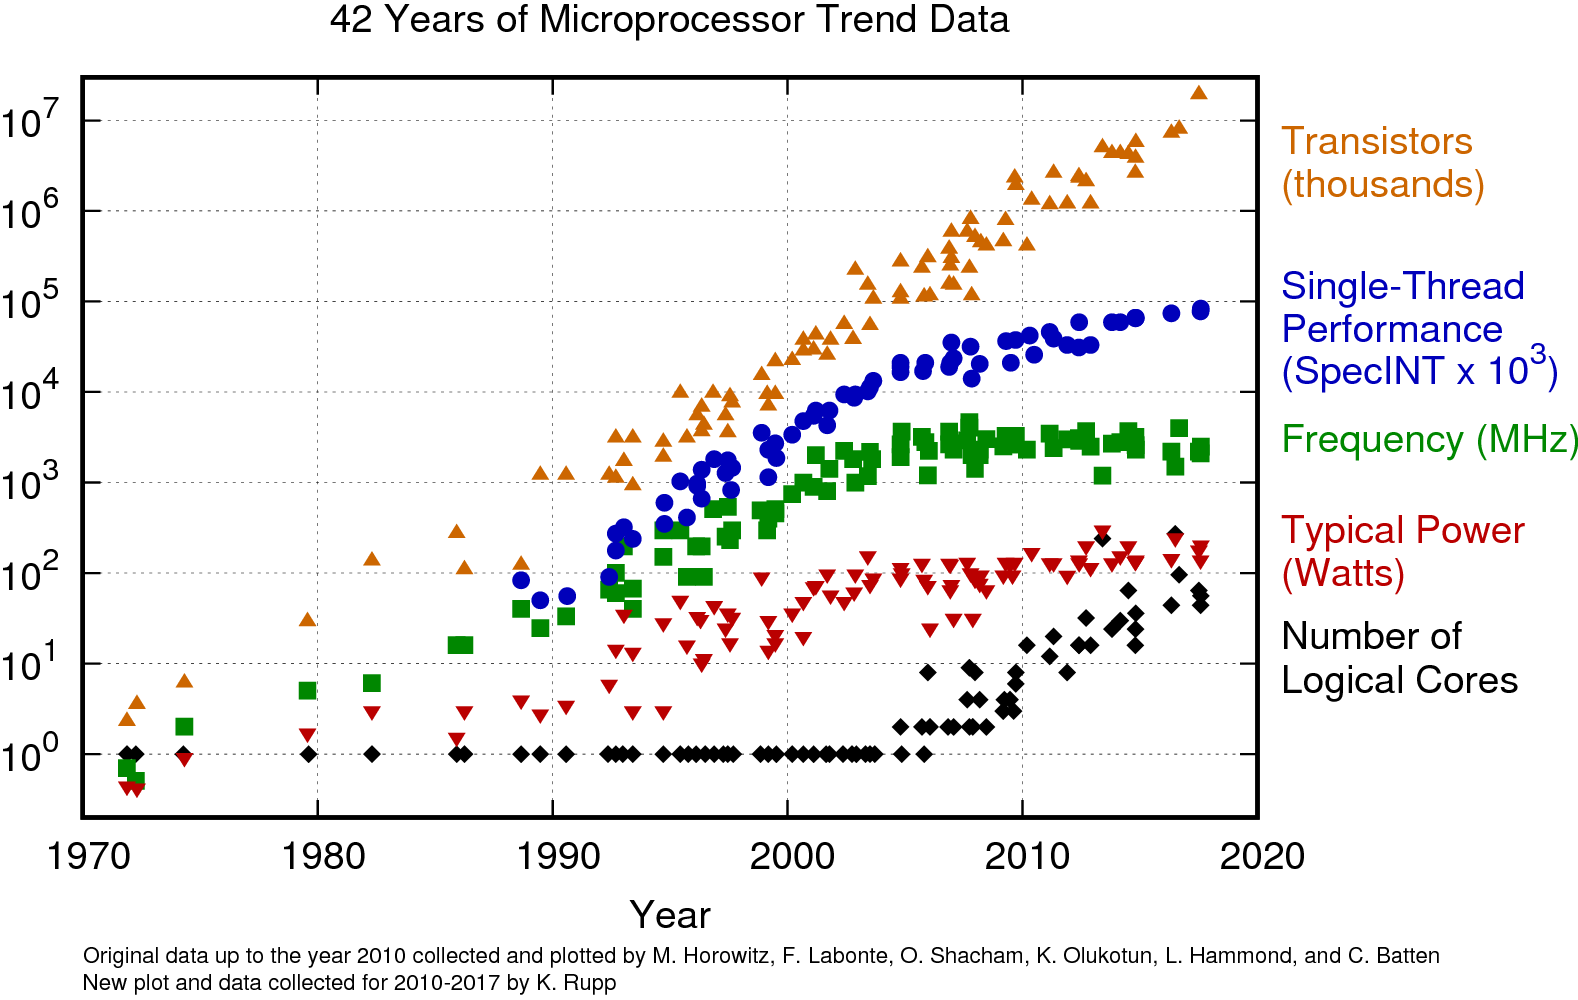
\includegraphics[width=\textwidth]{imagenes/chapter2/42-years-processor-trend.png}
    \caption{Evolución de los procesadores y sus principales factores. Extraído de~\cite{42-trend-data}.}
    \label{fig:42-trend-data}
\end{figure}

Debido a la barrera física con la que se enfrentan en caso de seguir con la misma estrategia, era necesaria la creación de sistemas más sofisticados de enfriamiento, como los que propuso \texttt{IBM} en su momento basados en enfriamiento liquido \cite{ibm-cooling}, lo que motivó la elección de una nueva dirección de desarrollo. Para mitigar y resolver este problema, en lugar de aumentar la frecuencia, se adoptó la idea de aumentar la cantidad de cores dentro del procesador, pero funcionando a frecuencias más bajas. Estrategia mejor conocida como \textit{multicore}, que al día de hoy se mantiene con fuerza siendo así inspiración para las arquitecturas paralelas como la GPU, que explota esta idea en gran escala. En particular, las GPUs han ido agregando más cores (funcionando a frecuencias bajas), entre otros factores que han permitido el aumento de performance de estos dispositivos. Dicha evolución vuelve a estos dispositivos una arquitectura muy atractiva en ámbitos de la computación científica.

La GPU y la CPU presentan grandes diferencias a nivel de arquitectura, ya que en la primera, la gran mayoría de los transistores están dedicados al cómputo mientras que en la última están dedicados a intentar mejorar el tiempo de ejecución secuencial. En una CPU tradicional, gran parte de los transistores están destinados a realizar otro tipo de tareas que el cómputo, como por ejemplo: 

\begin{itemize}
    \item predicción de branches: Para ejecutar secuencialmente y explotar las técnicas de \textit{pipelining}, es importante saber cuál instrucción es la siguiente a ejecutar, %  sino, la CPU esperaría hasta último momento el tiempo que le toma traer la instrucción, decodificarla y ejecutarla, quedando ociosa. 
    por lo que la CPU tiene mecanismos para intentar prever, por ejemplo, ante instrucciones condicionales, por cuál de estas ramificaciones podría seguir.
    \item prefetch de memoria: Cargar memoria, con datos que de antemano se sabe que la CPU va a necesitar o cree que puede llegar a utilizar, para no tener que esperar durante la ejecución la carga de esos datos.
    
    \item ejecución fuera de orden
    
    \item caché de datos
\end{itemize}

Entonces, la CPU se  encarga de todos estos detalles, dedicando gran parte de sus recursos, dando la impresión al usuario de que el sistema funciona más rápido.

En cuanto a las GPUs, estos conceptos no están presentes, o aparecen en menor medida,  dedicando la mayoría de los transistores al cálculo, agregando más unidades de cómputo. La Figura~\ref{fig:cpuvsgpu} muestra una comparativa aproximada de la proporción de transistores que está dedicado a cada componente dentro de una CPU y una GPU. Mientras que gran parte de la capacidad de las CPUs está dedicada a control, intentando mejorar el tiempo de ejecución secuencial, las GPUs enfocan estos transistores en agregar más unidades de cómputo, reduciendo las unidades de control. 

\begin{figure}
    \centering
    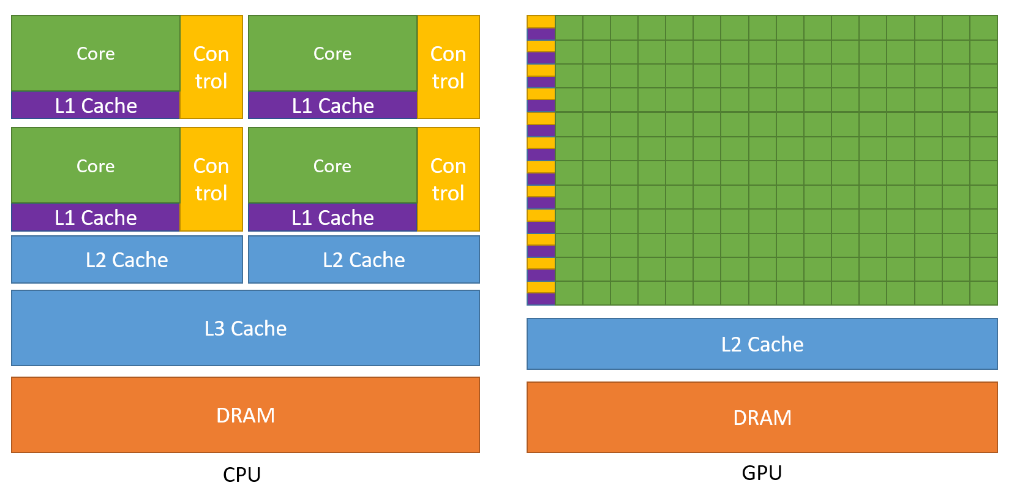
\includegraphics[width=\textwidth]{imagenes/chapter2/cpuvsgpu.PNG}
    \caption{Diferencia de arquitectura entre una CPU y una GPU. Extraído de~\cite{cuda-programming-guide}.}
    \label{fig:cpuvsgpu}
\end{figure}


Si se estudia la arquitectura de las GPUs, es necesario abordar también CUDA, %(sigla que abrevia Compute Unified Device Architecture)
%y su paralelismo o mapeo con las estructuras que este tipo de dispositivos (de la marca NVIDIA) ofrece.
término utilizado no solamente para describir la arquitectura de hardware presentada en 2006 por la compañía \texttt{NVIDIA}, sino también para referirse al modelo y lenguaje de programación que permite crear aplicaciones que ejecutan en estos dispositivos. 

Desde el punto de vista del modelo de programación, la ejecución del programa se distribuye en hilos (\textit{threads}), organizados en una grilla indexada llamada bloque (\textit{threadblock}), y a su vez, estos bloques también forman una grilla indexada (\textit{grid}). A priori, la ejecución de los hilos y bloques es totalmente independiente y puede darse en cualquier orden. El lenguaje de programación consiste en una extensión del lenguaje C, que permite, entre otras cosas, la creación de estas grillas de hilos, la programación de las funciones a ejecutar en el dispositivo (kernels) y las transferencias de datos entre la CPU y la GPU.

Por su parte, la arquitectura de hardware se forma entorno a una serie de multi-procesadores paralelos (Streaming Multiprocessors o SMs), cada uno formado por varios núcleos. La cantidad de procesadores y núcleos con los que cuenta la GPU varía según las diferentes generaciones de tarjetas. 
La memoria de las GPUs se organiza de forma jerárquica. En un primer nivel, existe una memoria global relativamente lenta pero accesible por todos los hilos. Se encuentra fuera de los multiprocesadores, por lo que el acceso a la misma implica una alta latencia, pero también posee un gran ancho de banda. Adicionalmente, a partir de la segunda generación de CUDA, se incluye una memoria caché de segundo nivel. Dentro de cada multiprocesador, existe una memoria de baja latencia pero de mucho menor tamaño con respecto a la global. Esta memoria es compartida físicamente por los bloques de hilos que residen en el multiprocesador. Por último, cada multiprocesador contiene un archivo de registros el cual es repartido entre todos los hilos residentes en el multiprocesador. Los registros son la memoria más rápida que brinda la GPU, pero también es la más reducida en tamaño.

Existe cierta correspondencia entre este modelo abstracto y la arquitectura de hardware. Siguiendo el espíritu de la clasificación de sistemas paralelos propuesta por Flynn en \cite{Flynn1972}, NVIDIA clasifica su arquitectura como Single Instruction Multiple Thread o SIMT. A diferencia de la categoría SIMD, en la cual una misma instrucción  se ejecuta simultáneamente sobre distintos elementos de un conjunto de datos, en SIMT el usuario puede  especificar distintos flujos de ejecución para los distintos hilos, aunque dadas las características  del hardware, el desempeño es mucho mayor cuando el comportamiento de la aplicación se asemeja al tipo SIMD.
 
Comenzada la ejecución del programa, cada multiprocesador se encarga de la ejecución concurrente de un grupo fijo de bloques, como se muestra en la Figura~\ref{fig:cuda-gpu}. Los hilos pertenecientes a estos bloques son divididos, planificados y ejecutados en grupos de 32 hilos llamados warps. La división se realiza siempre de forma que los hilos con índice 0 a 31 forman el primer warp, los de índice 32 a 63 al segundo, y así sucesivamente. La ejecución se organiza de forma que los threads de un mismo warp deben ejecutar la misma instrucción en cada momento. Dado el caso, si en el flujo de ejecución de distintos hilos del mismo warp, dos hilos divergen, debiendo ejecutar distintas instrucciones, las mismas se ejecutan de forma secuencial y los hilos que ejecutan una de las instrucciones quedan inactivos hasta que el resto de los hilos del warp ejecuten la otra instrucción. Por esta razón, la máxima eficiencia es alcanzada cuando todos los hilos de un warp ejecutan la misma instrucción en todo momento, aunque la misma se ejecute sobre distintos elementos del conjunto de datos. La asignación de recursos a cada warp dentro de un multiprocesador se realiza de forma estática, asignando un segmento del archivo de registros (\textit{register file}) a cada warp, y asignando una sección de la memoria compartida del multiprocesador a cada bloque que ejecuta en él. De esta forma, el cambio de contexto entre un warp y otro se realiza sin costo. 
Otro aspecto muy importante son los accesos a memoria. No sólo es una mejora importante que cada hilo de un mismo warp ejecute la misma instrucción, sino que es importante también que ejecuten utilizando datos que se encuentren en espacios de memoria contiguos, produciendo accesos \textit{coalesced}. El acceso a memoria \textit{coalesced}, refiere a combinar múltiples accesos a la memoria en una sola transacción. %Por ejemplo en las GPU K20, se puede acceder a 128 bytes contiguos (32 palabras en simple precisión) mediante un warp (32 hilos consecutivos) en una sola transacción. 


Junto con CUDA, NVIDIA provee un conjunto de herramientas que continúan en desarrollo gracias a los aportes de investigadores, las cuales tienen como objetivo complementar la arquitectura mejorando su usabilidad en distintas áreas de aplicación. Entre estas herramientas se encuentran lenguajes como \texttt{CUDA FORTRAN}, \texttt{PyCUDA}, APIs como \texttt{OpenACC} o \texttt{PGI Accelerator Compiler}, herramientas de análisis, debugging, y un gran conjunto de bibliotecas optimizadas en GPU, como por ejemplo \texttt{cuBLAS}~\cite{cublas} y \texttt{cuSPARSE}~\cite{cusparse}.


\begin{figure}
    \centering
    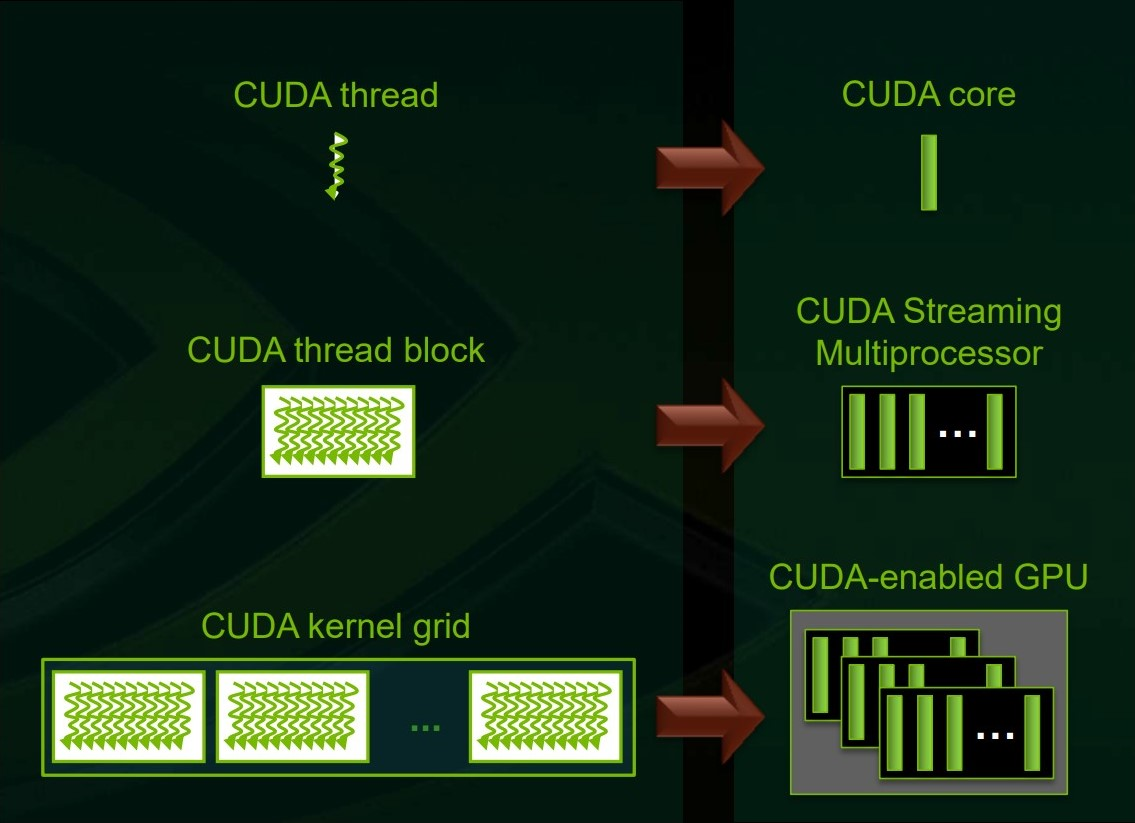
\includegraphics[width=0.7\textwidth]{imagenes/chapter2/cuda-gpu.jpg}
    \caption{Mapeo entre estructuras CUDA y GPU. Extraído de \cite{cuda-programming-guide}.}
    \label{fig:cuda-gpu}
\end{figure}


\subsection{Algoritmos en HPC}

En general, el cuello de botella de la mayoría de las operaciones y algoritmos que se ejecutan en arquitecturas de HPC al día de hoy, se da en los accesos a memoria, debido principalmente a la alta latencia de los mismos en relación a la de las %o ancho de banda significativamente más lento que estas presentan con respecto a la cantidad de 
operaciones aritméticas (operaciones en punto flotante FLOPS). Muchos cálculos científicos sólo aprovechan una fracción de la potencia computacional en las arquitecturas de alto rendimiento actuales. La dificultad radica, en muchos casos, en mapear dichas operaciones a las arquitecturas, intentando explotar al máximo los atributos de cómputo que presentan haciendo uso de, por ejemplo, jerarquías de memoria con el objetivo de mitigar la baja latencia de las memorias principales.

Al mismo tiempo, las operaciones de memoria son el principal consumidor de energía de las arquitecturas modernas, lo que afecta en gran medida el costo de los recursos, como se puede observar en la Figura~\ref{fig:horowitz-energy}. Un estudio  detallado de este y otros problemas es el que plantea Horowitz en~\cite{Horowitz2014}.

\begin{figure}
    \centering
    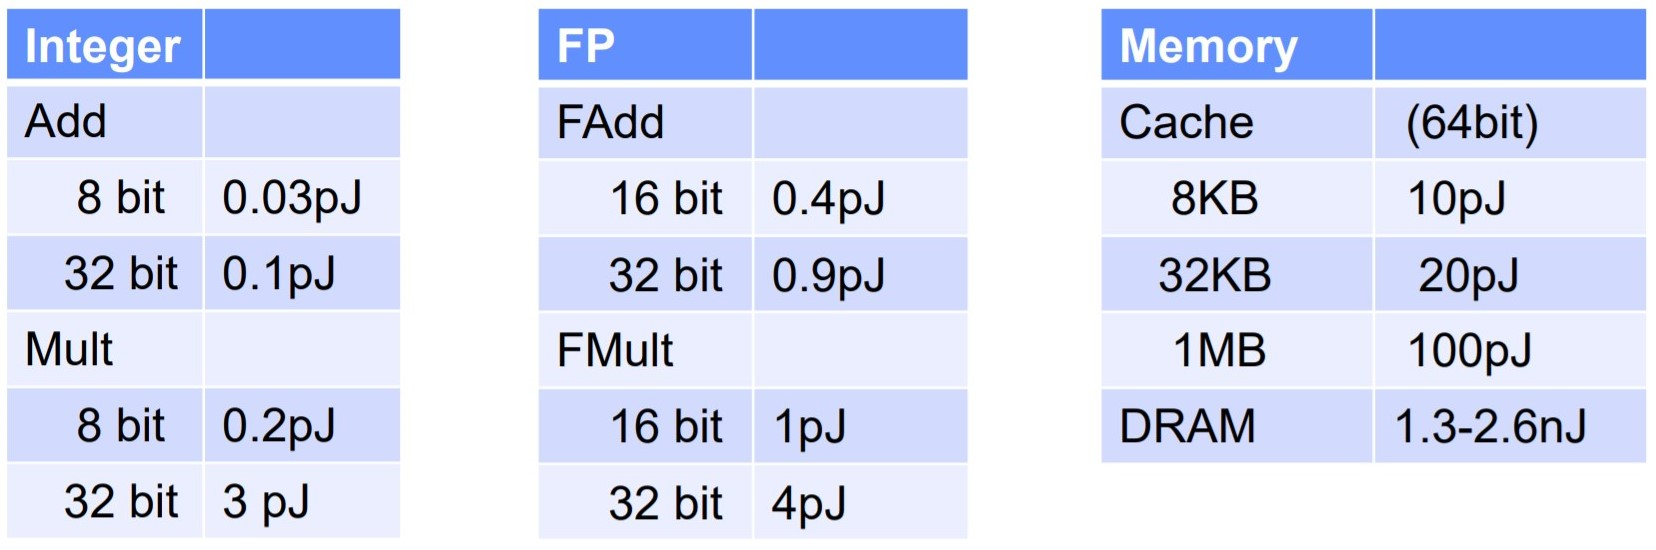
\includegraphics[width=\textwidth]{imagenes/chapter2/horowitz-energy.jpg}
    \caption{Valores aproximados de energía consumida por operación (45nm). Extraído de~\cite{Horowitz2014}.}
    \label{fig:horowitz-energy}
\end{figure}

El ALN no escapa de este paradigma, en particular, las operaciones con matrices dispersas encajan perfectamente en esta categoría de problemas. Entre los varios problemas del ALN dispersa, la SpMV es un claro ejemplo de operación con un costo computacional razonable a nivel de operaciones, y que puede ser atacada de forma paralela, pero que se ve fuertemente limitada por el ancho de banda entre procesador y memoria, 
además su baja intensidad computacional, es decir, la baja cantidad de operaciones aritméticas realizadas por cada acceso a memoria, sumada a la aleatoriedad de los accesos que implica un pobre aprovechamiento de los caches, produciendo un ratio bajo de lecturas efectivas.

En este contexto, es de gran interés estudiar formatos ``óptimos'' para matrices dispersas, que logren reducir la cantidad de transacciones de memoria o, al menos, ofrezcan mejoras mediante el acceso de forma ordenada, aprovechando así en lo posible el ancho de banda limitado.





	% Se carga el capítulo 02
     \chapter{Revisión del estado del arte}\label{ch:estado-del-arte}
% El objetivo de este capítulo es justificar el diseño metodológico elegido. La finalidad de una metodología bien descrita es explicitar los pasos mediante los cuales se obtienen los resultados, y por tanto el cumplimiento (o no) de los objetivos establecidos, de manera tal que pueda ser replicado por otro investigador. Si corresponde, también se evaluarán problemas metodológicos y se realizarán consideraciones éticas.
% En algunas disciplinas este capítulo se denomina Materiales y métodos. 
% En caso de que la investigación sea de carácter experimental, se debe especificar la siguiente información:


% Quizas discutir la cantidad de papers que hablas de mejoras sobre CRS para spmv sobre GPUs
% LightSpMV: faster CSR-based sparse matrix-vector multiplication on CUDA-enabled GPUs
% Efficient CSR-Based Sparse Matrix-Vector Multiplication on GPU
% A novel CSR-based sparse matrix-vector multiplication on GPUs

% Precisiones mixtas
%https://www.researchgate.net/publication/276902250_Acceleration_of_GPU-based_Krylov_solvers_via_data_transfer_reduction
%https://www.researchgate.net/publication/46390954_An_Error_Correction_Solver_for_Linear_Systems_Evaluation_of_Mixed_Precision_Implementations

% Reordering
% https://www.researchgate.net/publication/290192543_A_systematic_review_of_heuristics_for_symmetric-matrix_bandwidth_reduction_methods_not_based_on_metaheuristics_A_systematic_review_of_heuristics_for_symmetric-_matrix

% Optimizaciones
% https://www.researchgate.net/publication/283658949_A_lightweight_optimization_selection_method_for_Sparse_Matrix-Vector_Multiplication





Como se mencionó anteriormente el uso de matrices dispersas tiene múltiples aplicaciones en el ámbito de la ciencia y la ingeniería, desde simulaciones de circuitos electrónicos~\cite{Davis2010Algorithm9K}, pasando por problemas de optimización y hasta operaciones con grafos de redes sociales~\cite{Chakraborty2018}. En este contexto, también tratado brevemente en la Sección~\ref{spmv}, una de las principales operaciones involucradas es la Multiplicación Matriz dispersa-Vector (SpMV). Esto ha motivado que en los últimos 40 años muchos trabajos busquen optimizar la SpMV para poder atacar de forma más eficiente los problemas. 

En la literatura se encuentran varios trabajos centrados en el diseño de formatos de almacenamiento que buscan optimizar diferentes aspectos de la SpMV\footnote{Aunque el proyecto no se centra en el estudio de formatos para una operación específica, la concentración de esfuerzos en la operación SpMV implica un lógico destaque.}. Algunos de estos esfuerzos avanzaron en la implementación de formatos híbridos en~\cite{Maggioni2014}, mientras que otros se concentraron en reducir la precisión de los números utilizados~\cite{Xu2010}, buscando aprovechar mejor el ancho de banda de acceso a memoria. Las motivaciones para utilizar formatos novedosos son diversas. Mientras que, en ocasiones, se busca acotar el espacio de almacenamiento, implicando una posible reducción en los accesos a memoria, en otros casos el objetivo es mejorar alguna característica del cómputo de una operación específica, incluso para sacar partido de las características de determinado hardware. Por ejemplo, si se consideran los formatos de almacenamiento clásicos como COO y ELLPACK, que se utilizan para representar matrices dispersas, estructuras de datos como estas suelen emplear matrices con índices para el acceso indirecto a los vectores densos de entrada. Para cada operación de suma o multiplicación, ELLPACK requiere tres accesos a la memoria, mientras que para COO, son necesarios cuatro accesos. Debido a la baja relación entre las operaciones de punto flotante y el número de accesos a la memoria, el rendimiento de la SpMV generalmente está limitado por el ancho de banda de memoria disponible en la arquitectura subyacente.


% HABLAR DE QUE ESTAS OPERACIONES ESTÁN LIMITADAS POR MEMORIA, ACCESOS A MEMORIA, limitada por ancho de banda BANDWIDTH
% El versito de siempre 

A continuación se presentan, de forma breve, las ideas abordadas en diferentes investigaciones que intentaron avanzar en las capacidades de los formatos dispersos. % algunos buscando mejorar cantidad de accesos a memoria, almacenamiento (al final es lo mismo....? dependerá de como sena los accesos si son coalesced? ) y otros mejorar como se menciona anteriormente, en optimizar operaciones SpMV (principalmente en GPUs?).
% Este capítulo se puede considerar una extensión del Capítulo~\ref{ch:fundamento-teorico}, pero profundizando en conceptos avanzados y con foco en las técnicas que sacan partido de los formatos de almacenamiento. 
Si bien, en muchos casos, todos los conceptos abordados en este capítulo están fuertemente relacionados, se decidió clasificar los esfuerzos bajo las siguientes categorías: formato de almacenamiento por bloques, formatos híbridos, uso de múltiples precisiones y técnicas de reordenamiento, únicamente con la intención de organizar el estudio. 


%\section{Formatos de compresión}

% \subsection{Formatos híbridos}
\section{Estrategias de almacenamiento por bloques}

Belgin et al. \cite{Belgin2009} presentan un enfoque llamado \textit{Pattern-based Representation} (PBR), basado en identificar patrones de bloques, es decir, elementos no nulos agrupados en una zona pequeña de la matriz y reemplazar los índices de los elementos no nulos por máscaras en forma  de bitmaps para reducir la sobrecarga del ancho de banda producida por los accesos a los índices para la mayoría de las matrices dispersas.
Esta reducción se da debido a que, en lugar de un índice por elemento no nulo de la matriz, las representaciones por bloques emplean un índice por dicha subestructura. Sin embargo, la utilización de estrategias por bloques puede requerir un llenado  explícito de elementos nulos (también llamado \textit{zero-filling}), lo que puede aumentar los requerimientos de memoria y las operaciones en punto flotante. Por este motivo, este tipo de técnicas suelen ser útiles únicamente cuando la matriz presenta cierta estructura de bloques densos.
% Este artículo presenta una representación que los autores llaman PBR, o \textit{Pattern-based Representation}, que busca reducir la sobrecarga del ancho de banda producida por los índices para la mayoría de las matrices dispersas, sin aplicar \textit{zero-filling}) y sin requerir de la existencia de subestructuras densas. 
PBR explota un análisis simple que identifica estructuras de bloques recurrentes que comparten el mismo patrón de coeficientes no nulos dentro de una matriz. Para cualquier patrón que cubra más que un número umbral de no nulos, PBR representa la submatriz formada por este patrón en el formato (BCOO), junto con una máscara de bits que describe el patrón repetido.
Para la identificación de los patrones repetidos, se utiliza una estrategia de análisis simple. Dado un bloque de tamaño $R \times C$, se divide la matriz de dimensiones $m \times n$ en una grilla de $\lceil {\frac{m}{R}} \rceil \times \lceil{\frac{n}{C}}\rceil$ bloques rectangulares, contando cuán frecuente es cada una de las combinaciones, entre las $2^{R \times C}$ posibles. Luego se representa la submatriz correspondiente a cada bloque con un patrón, registrando las coordenadas del bloque en formato COO, junto con un ``bloque código'', que es un vector de bits de tamaño $R \times C$ que codifica el patrón de los elementos no nulos. Los autores dan dos variantes para la implementación de la SpMV utilizando PBR: una secuencial y la otra paralela. En la estrategia paralela, se divide la matriz en particiones, asignando una a cada hilo. Además, %a diferencia de otras implementaciones por ejemplo, basadas en CSR, no es posible realizar una partición por filas que permita acceder al vector $y$ a través de cada hilo, entonces para evitar costosas sincronizaciones, los autores proponen que 
cada hilo mantiene un vector $y_{i}$ que representa el producto de $A_{i}x$ correspondiente a la submatriz que tiene asignada, realizando la adición de los distintos $y_i$ mediante una reducción paralela al final. 
En cuanto a la evaluación, los autores reportan una reducción en el tiempo de ejecución al realizar operaciones como SpMV basadas en PBR, tanto en secuencial como en paralelo.
Quizás como desventaja se podría destacar que PBR puede interferir en el principio de localidad de los accesos al vector $x$. Como ventaja, PBR no realiza asunciones sobre el patrón y la estructura de la matriz a la hora de identificar los bloques por patrón.

En otra investigación, Choi et al.~\cite{Choi2010} proponen técnicas de auto-ajuste para los parámetros como, por ejemplo, el tamaño de bloques en el formato BCSR basados en modelos del desempeño de la SpMV en GPUs. Posteriormente, presentan una implementación de un nuevo formato de compresión para matrices dispersas que denominaron \textit{blocked} ELLPACK (BELLPACK) que combina las ventajas de sub-bloques densos de BCSR y la comodidad de los accesos por vector de ELLPACK.
En sus primeros resultados observaron que si bien BCSR presentaba mejoras con respecto a CSR, igualmente no competía con la mejor implementación de la biblioteca cuSparse de NVIDIA, que en la mayoría de casos es HYB. 

De forma similar a~\cite{Choi2010}, Yan et al.~\cite{Yan2014} proponen basados en bloques, con el objetivo de optimizar la SpMV, una extensión de un formato clásico, en este caso COO. Los coeficientes, agrupados en bloques, son almacenados con un índice de columna y de fila, de modo de reducir la sobrecarga producida por los accesos a índices distintos, como a direcciones no contiguas. En esta investigación presentan dos variantes para COO, la primera, denominada blocked compressed common coordinate (BCCOO). 
Utiliza bits flags para reducir la sobrecarga de los accesos por índice de fila. Indicando con un bit en 1 el inicio de una fila de bloques.

Luego, para mejorar la tasa de aciertos de la caché para acceder al vector multiplicado, proponen la segunda estrategia de almacenamiento, en la que se divide la matriz dispersa en slices verticales y estos son alineados antes de aplicar el formato BCCOO. Dicha variante con en particiones verticales, se conoce como formato BCCOO+.

\section{Formatos híbridos}

En esta sección se analizan propuestas de formatos dispersos basados principalmente en combinar formatos existentes. Notar que si la matriz $A$ puede ser expresada, por ejemplo, como  $A = A_\alpha + A_\beta$, entonces $Ax = A_\alpha \cdot x + A_\beta \cdot x$. Esta descomposición permite almacenar ambos sumandos en un formato distinto con el objetivo de optimizar el desempeño de las operaciones.

Quizás una de las primeras ideas de utilizar estrategias híbridas se puede encontrar en las técnicas que guardan la diagonal de la matriz en un vector separado del resto de la matriz. Esta estrategia es especialmente útil cuando se aplican precondicionadores sobre la diagonal en los métodos iterativos de resolución de sistemas lineales. 
Similar a esta idea,\ los autores Sun et al. presentan, en su investigación~\cite{Sun2011}, el formato Compressed Row Segment with Diagonal-pattern (CRSD). En su planteo, centrado principalmente en matrices con patrones diagonales, agrupando o segmentando por filas, proponen almacenar las componentes diagonales en vectores cuyo índice corresponde al offset con respecto a la diagonal. Si la diagonal a almacenar se encuentra por encima de la principal tendrá un offset positivo, negativo cuando está por debajo. 
\begin{figure}[h]
    \centering
    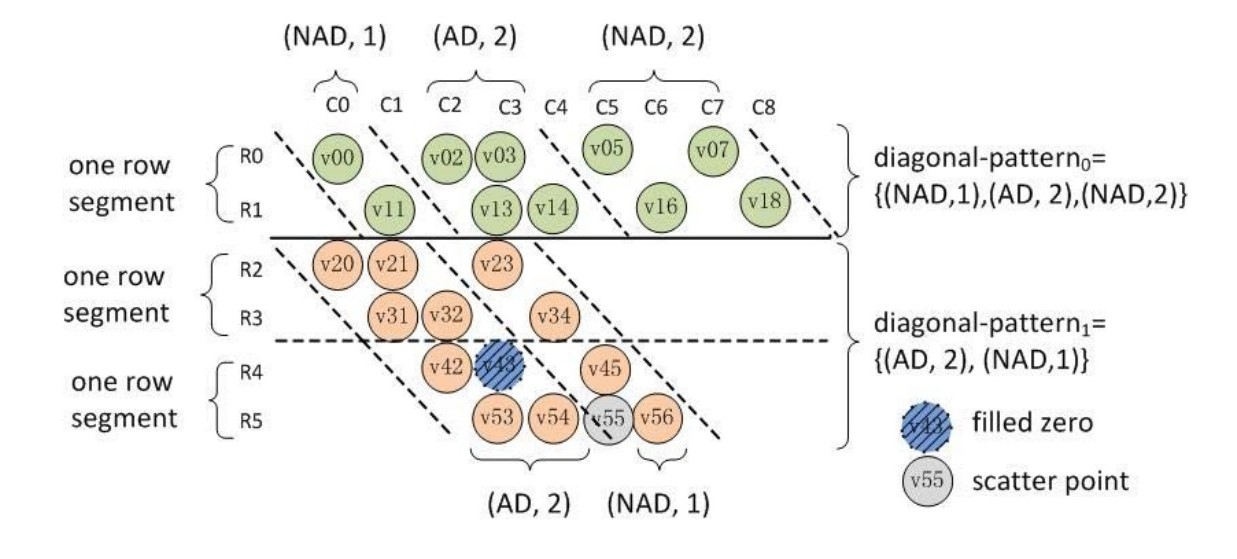
\includegraphics[width=.8\textwidth]{imagenes/chapter3/crsd.jpg}
    \caption{Sección de matriz diagonal, aplicando conceptos del CRSD. Extraído de~\cite{Sun2011}.}
    \label{fig:CRSD}
\end{figure}
Excepto por los elementos más dispersos de la matriz, fuera de diagonales densas, la matriz es almacenada a través de patrones diagonales. Aquellas filas que poseen estos elementos dispersos, o como los denominan los autores scatter point, aquellos que están presentes en una sola diagonal, son agrupadas y almacenadas en forma completa con el formato ELL, debido a que de no utilizar otro formato, sería necesario realizar \textit{zero padding} agregando overhead al procesamiento y trabajo con la matriz. Esta idea puede ser observada mejor en la Figura~\ref{fig:CRSD}.


Otro ejemplo puede ser el formato HYB que combina los formatos ELL y COO, propuesto por Bell y Garland~\cite{Bell2009}. % o modificaciones (mejoras) a formatos existentes dando lugar a formatos nuevos (CoAdELL). 
Este formato busca mitigar ciertas debilidades del esquema ELL, que si bien ofrece ventajas en cuanto a la localidad de datos, es poco eficiente en los casos donde la cantidad de elementos no nulos en cada fila varía considerablemente. En tales circunstancias, 
% con respecto al promedio de este valor por fila, se puede observar que es poco eficiente. Dado el caso, al utilizar este formato se da una caída de desempeño general de los algoritmos, basado en que 
hay un aumento significativo del espacio total requerido (debido al padding necesario para completar los vectores de cada fila con menos de $k$ elementos no nulos, donde $k$ es la cantidad máxima de elementos en una fila de la matriz). Notar además, que los algoritmos operan con estos valores agregados aún siendo nulos.
Para trabajar con estas matrices de forma más eficiente, una opción es utilizar un formato híbrido, que divida la matriz en dos, una componente en formato ELL y la otra por ejemplo en COO. La idea es tener una matriz $A_{ELL}$ de tamaño $n\times k$ donde la cantidad de elementos por fila se aproxime bastante a $k$ y otra matriz $A_{COO}$ para el resto de los elementos. 
% Estas ideas, entre otras, motivaron el formato HYB. %Un ejemplo de matriz dispersa representada en este formato se puede ver en la Figura \ref{fig:hyb-format}.
Elegir la columna $k$ que determine la partición, se puede resolver, como en la implementación de la biblioteca \textit{CUSP}~\cite{cusp-bell}, con una heurística donde dicho valor se elige de forma de que el número de filas con al menos $k$ elementos no nulos, sea menos de un tercio de la cantidad total de filas de la matriz.



Otra investigación donde se combinan dos formatos de almacenamiento de matrices dispersas, enfocadas en mejorar el desempeño de la SpMV en GPUs, se puede encontrar en~\cite{Guo2015}, en la cual Guo et al. presentan ELL and Vectored CSR Hybrid (EVC-HYB). 
El formato presentado se construye primero aplicando reordenamientos simples entre filas basado en los largos de éstas (\nnz por fila), de menor a mayor, y seguido, se realiza una partición en dos grupos, filas largas y cortas. Centrado en esta partición, las entradas de la matriz son almacenadas en los formatos ELL o VCSR\footnote{Vectorized CSR, implementación vectorizada de la SpMV optimizada para GPUs utilizando el formato CSR.} según corresponda. Ambos formatos funcionan bien para ciertos tipos de clases de matrices, por ejemplo, ELL funciona bien con las matrices cuya cantidad de elementos no nulos por fila  es baja y similares entre sí, debido a la localidad de los accesos, en cambio, es muy ineficiente cuando esta cantidad varía considerablemente entre las filas. Mientras que VCSR funciona mejor con matrices cuyas filas son de cierto largo suficiente y en lo posible múltiplos de 32 (warp en GPU), pero la propiedad de los accesos coalesced no puede ser explotada de forma óptima si las filas son de largos menores, particularmente menores a 16. Entonces, buscando aprovechar los beneficios que estos formatos presentan y evitar las debilidades, los autores plantean la estrategia híbrida EVC-HYB que combina ambos. Para la evaluación, en el estudio se comparan contra las mejores elecciones de CUSP para la SpMV, que en general son, CSR y HYB. Evaluaron, para 22 matrices distintas tomadas de la SSMC, la cantidad de operaciones punto flotante por segundo (FLOPS) en 500 iteraciones utilizando los diferentes formatos, obteniendo sin aplicar reordenamientos, mejoras en velocidad de hasta $1,64$, también con resultados que degradaron la cantidad de operaciones, que en el peor de los casos se registraron reducciones en un factor de $0,90$. 

% EL PORQUE DEL HYB (hybrid format propuesto por  Bell and Garland)
% Este formato es poco eficiente cuando la cantidad de elementos no nulos en cada fila varia considerablemente respecto al promedio de elementos no nulos por fila. Dado el caso, hay una pérdida en términos del espacio necesario para almacenar la matriz, asi como 

% Como producto de modificaciones de de formatos existentes, que dieron lugar a estructuras nuevas, a continuación, se estudia el caso del formato 


% CoAdELL, 

% Basado en ELL, formato discutido en~\ref{ell}, se desarrolla CoAdELL, un formato disperso con el que se obtuvo resultados interesantes en la implementación SpMV en GPU. 

% La idea ``innovadora'' , con respecto a su antecesor AdELL, es usar una codificación basada en la distancia entre elementos no nulos. Las distancias entre dos elementos no nulos consecutivos, comunmente, puede ser representada utilizando enteros pequeños, bastando con representaciones de 8-bits o 16 bits para las matrices mas grandes y dispersas.

% AdELL propone, basados en warp gained ELL? (sliced ELL), balancear las cargas entre los warps. Dividiendo la estructura en varias estructuras ELL independientes.....



\section{Múltiples precisiones}\label{multiple-precision}


Operaciones como la SpMV, limitadas por el acceso a memoria~\cite{Goumas2008}, pueden obtener un beneficio inmediato si se logra reducir el uso de memoria en el almacenamiento. El simple hecho de sólo indexar los datos asociados a los elementos no nulos supone una oportunidad para la compresión de estos datos. La mayoría de los formatos dispersos, tienen cierto grado de compresión en los índices. Por ejemplo:  los formatos basados en ELL (ver Sección \ref{ell-format}) no almacenan explícitamente un índice para las filas, sino que este se infiere por la posición en la memoria. Otros formatos en bloque guardan un índice asociado a cada sub-bloque denso (en lugar de almacenar un índice por cada valor no  nulo, reduciendo los datos de indexación) y luego con un desplazamiento acceden a los valores dentro de éste.

El uso de múltiples precisiones es una idea muy empleada en la historia del ALN. En general, centrado en la precisión de los coeficientes de las matrices, tanto por motivos de almacenamiento (por ejemplo trabajar en simple precisión reduce a la mitad el almacenamiento) como de cómputo (en una CPU la relación de desempeño entre simple precisión y doble precisión es 2 a 1 pero en otras plataformas de hardware, como por ejemplo algunas GPUs, las diferencias suelen ser mucho mayores).
En el caso del ALN disperso, es aún mayor la motivación para disminuir la precisión, dado que la principal restricción para el desempeño son los accesos a memoria, por lo que trabajar con precisiones menos demandantes disminuye la cantidad de datos que se mueven por la jerarquía de memorias.

En los últimos años, en el ALN dispersa, han aparecido varios esfuerzos por trabajar con precisiones reducidas o modificaciones de los formatos utilizados. Algunos ejemplos de estos esfuerzos son \cite{Anzt2018, Goebel2020}, donde se evalúa cómo el uso de precisiones reducidas (como half y single) para almacenar algunos coeficientes de los precondicionardores obtenidos con el método de Jacobi, mejora el desempeño al utilizarlos en métodos iterativos para resolver sistemas de ecuaciones lineales.
Específicamente, estos formatos buscan reducir el overhead producido por la transferencia de datos, almacenando adaptativamente los bloques diagonales del precondicionador de Jacobi en distintas precisiones.
En \cite{Grtzmacher2019, Grtzmacher2020} se aplican ideas similares, pero desacoplando el formato de punto flotante utilizado para operaciones aritméticas del formato utilizado para almacenar los datos en la memoria. %, basados en la segmentación o división de la \texttt{mantissa} de los formatos del estándar IEEE,  un formato adaptable de modo que se pueda acceder a los valores con una latencia menor, si se acepta trabajar con una precisión reducida a la hora de obtener resultados, útil para problemas que permiten cierto margen de error o que trabajan con valores acotados.

Un enfoque complementario, es reducir la precisión de los índices asociados a los coeficientes. En este sentido, en el trabajo de Shiming Xu et al. \cite{Xu2010} se propone una optimización de la SpMV, tomando como base el formato ELL, cuyo objetivo es disminuir la cantidad de bits necesarios para representar los índices. En este sentido, se estudia la posibilidad de utilizar como índice de la columna la distancia a la diagonal en lugar del valor real de la coordenada atacando, en este caso, un conjunto acotado de matrices cuadradas de tamaño $n\times n$, donde se busca reducir la distancia de los elementos no-nulos a la diagonal a través de reordenamientos o permutaciones como el método RCM (Reverse Cuthill-McKee). Este trabajo será discutido y analizado con mayor profundidad en la Sección~\ref{sec:reord}.%Habiendo reducido el ancho de banda, proponen la utilización de precisiones reducidas para almacenar los índices.


% \resumen{CoAdELL, utiliza codificacion diferencial, entre dos elementos no nulos de la misma fila}


Otra idea, es la planteada en el formato CoAdELL \cite{Maggioni2014}, donde se continúa la investigación realizada por los mismos autores \cite{AdELL-Maggioni2013}, centrada en la división por warps de los cómputos con matrices almacenadas en formatos basados en ELL. Esta mejora consiste en una técnica de compresión para reducir el almacenamiento asociado a los índices de columna. La idea es utilizar una codificación basada en la diferencia entre los índices de dos elementos no nulos consecutivos en una misma fila, técnica que la mayoría de autores denomina \textit{delta encoding} o \textit{delta compression}, también utilizada con frecuencia en otros campos de estudio~\cite{Ma2010}. Como estas distancias o deltas tendrán valores menores que los índices, se podrán representar con menor cantidad de bits. Por ejemplo, la secuencia 1,~2,~3,~4,~10, de índices de columna, pasa a valer 1,~1,~1,~1,~6. Se intenta entonces, estudiar la posibilidad de una compresión basada en la reducción de precisión de los nuevos coeficientes obtenidos aplicando esta técnica de codificación. %Si bien en el proyecto no se tomó en consideración por cuestiones de practicidad, notar, que esta técnica  puede ser levemente mejorada si se asume un 1 implícito en cada uno de los términos de la secuencia (menos para el primer elemento), dando por resultado la secuencia 1,~0,~0,~0,~5, tal y como se aplica en~\cite{Stevenson2012}.

% Para poder implementar eficientemente estas ideas en hardware masivamente paralelo tiene que ser posible deshacer las convergencias en paralelo. En otras palabras, necesitan la ejecución independiente de los hilos para proporcionar una ejecución adecuada en la GPU. Suponiendo que cada hilo se encarga de procesar, en la SpMV, una entrada del vector $y$, es decir tiene la tarea de computar las sumas y multiplicaciones de una fila de elementos no nulos de la matriz $A$ por las entradas del vector columna $x$.
% Como este hilo sólo procesa sus elementos no nulos, es capaz de calcular el índice de cada entrada a partir de la entrada no nula anterior (implicando, posiblemente, que al menos el primer índice de columna sea almacenado  con una cantidad mayor de bits, por ejemplo 32). %Explican también, que dicha técnica de compresión se acopla  muy bien con estructuras que aplican division por warps, basadas en ELL. Dado un warp en memoria, casi que se puede asumir que cada hilo dentro del warp procesa secuencialmente sus elementos no nulos. 
% Basados en AdELL \cite{AdELL-Maggioni2013}, cada warp está asociado a una estructura ELL ``independiente''. Permitiendo también aplicar de forma selectiva la técnica de compresión por índice de columna a cada warp, dependiendo si todos los delta (diferencias) pueden representarse con 8 o 16 bits. 
% Cabe resaltar que, posiblemente se necesite realizar algún tipo de padding entre el final de un warp ``comprimido'' y el siguiente para garantizar la alineación de 128 bytes.





En otro trabajo, Kourtis et al.~\cite{Kourtis2008} emplean de manera similar la compresión de datos de índice, esta vez buscando reducir la sobrecarga producida
por los mecanismos de descompresión debido a las predicciones erróneas de los flujos de cómputo de la operación. En particular, proponen dos métodos distintos apuntando a comprimir tanto índices como coeficientes no nulos utilizando el formato CSR como base para la investigación, los autores plantean mecanismos para la compresión y descompresión con el objetivo de optimizar la SpMV, atacando primero los índices de columna, estrategia que denominaron CSR Delta Unit (CSR-DU) y luego los coeficientes no nulos con otro formato que llamaron CSR Value Indexed (CSR-VI).  Intentando explotar la distribución por columnas de los elementos no nulos, como se ha estudiado anteriormente utilizan la codificación delta, calculada como la diferencia de índice con respecto al elemento anterior, agregando a esta estrategia la idea de división o agrupamiento por unidades con largos variables, dónde cada una se representa con la cantidad de bits necesaria para el máximo valor de la unidad. Esta compresión trae consigo un cierto overhead en la etapa interna de la SpMV producido por la decodificación dependiendo de la cantidad de bits utilizada. Si los coeficientes fueran comprimidos todos por separado produciría, casi con total seguridad, ramificaciones en la multiplicación, degradando el rendimiento de toda la operación. Entonces, cabe destacar que la decisión de cómo es conformada cada unidad, es decir su tamaño, es de gran impacto en la estrategia. Por ejemplo, si las unidades son muy pequeñas la sobrecarga generada por las divergencias en la descompresión superará a las ganancias que se puedan obtener al comprimir. En cambio, si el tamaño indicado es muy grande, es probable que se encuentren menos oportunidades de compresión debido a que un delta grande impactaría en la cantidad de bits del resto de los índices de la unidad que podrían admitir precisiones menores.


Generalmente, la carga de trabajo de los distintos métodos se concentra en el procesamiento de los valores en punto flotante, ya que normalmente estos se almacenan en doble precisión utilizando 64 bits. Sin embargo, pese a que la ganancia al aplicar compresión es potencialmente mayor, 
% Generalmente, los elementos no nulos de la matriz constituyen la mayor parte del conjunto de trabajo de cuando se utiliza algún formato de compresión, en este caso CSR, principalmente porque requieren 64 bits para ser representados. Por tanto, abordan la compresión desde la premisa de que hay mucho más que ganar con la compresión de los valores que con los índices en términos de reducción del conjunto de trabajo. Sin embargo, 
la compresión de valores en punto flotante no es tan sencilla como la de los números enteros (que permiten en algunos casos reducciones en la cantidad de bits si se conoce los rangos en los que estos trabajan), porque las operaciones aritméticas de punto flotante producen resultados redondeados, y reducir entonces la cantidad de bits implica posiblemente una pérdida de precisión. Pese a esto, los autores indican que existe un número significativo de matrices del conjunto experimental elegido en las que sólo una pequeña parte de sus valores son únicos. Esta redundancia puede ser explotada entonces, almacenando de forma única los valores comunes o repetidos y sus correspondientes referencias o punteros a su ubicación en la matriz, lo que conducirá a la reducción del conjunto de trabajo si la cantidad de valores redundantes es alta en relación al total.  En consecuencia, una reducción considerable en este aspecto, derivará en una mejora del rendimiento en caso de poder compensar el costo derivado de la indirección en el acceso a los valores redundantes.

Las ganancias en desempeño a la hora de utilizar CSR-DU, según los autores,  dependen del porcentaje del tamaño de información de índices sobre el tamaño total de la matriz. En el caso de matrices indexadas con 32-bits que contienen los valores numéricos en 64-bits, el porcentaje es cercano a $1/3$, por lo que la ganancia está limitada por este factor.

% Como se menciona anteriormente, los valores numéricos o coeficientes de la matriz son más difíciles de comprimir debido a principalmente dos razones, la pobre regularidad que éstos presentan y a los límites impuestos por la representación en punto flotante si no se acepta una pérdida de precisión.

Como conclusión general, % en la gran mayoría de las investigaciones se estudia el impacto de la compresión sobre la SpMV. Entonces, 
una técnica de compresión puede ser beneficiosa para la SpMV siempre y cuando el método de descompresión no atosigue al procesador con ramificaciones adicionales irregulares y difíciles de predecir. Como se muestra en~\cite{Goumas2008}, el kernel SpMV es muy sensible a operaciones extra, así como predicciones erróneas en branches pueden fácilmente dañar el desempeño.


Tang et al. \cite{Tang2013} proponen utilizar una familia de esquemas de compresión eficientes, que denominan  \textit{bit-representation optimized} (BRO), para reducir la cantidad de bits requerida para representar los índices. 
% que generalmente contienen una gran cantidad de información redundante, utilizando un formato de representación de bits eficiente. 
En particular, para el diseño de los esquemas de almacenamiento BRO, los autores tomaron en consideración aspectos importantes relacionados con las arquitecturas para las que fueron diseñadas las estrategias. Sin entrar en detalles de implementación, los autores se plantean estudiar el impacto de las etapas necesarias para aplicar estas técnicas. Por ejemplo, para poder realizar la descompresión en GPU, ésta debe ser relativamente liviana en comparación con las operaciones de suma  y multiplicación de la SpMV, de forma que la mayoría de los ciclos de la GPU se asignen a un trabajo útil y no se utilicen únicamente para descomprimir los datos del índice. Además, debido a que las GPU no contienen hardware complejo para la predicción de branches, la descompresión debe evitar los costosas penalizaciones por divergencia dentro de cada warp. 
En este sentido se presentan dos técnicas de compresión de índices, BRO-ELL y BRO-COO, basadas en los formatos ya estudiados ELL y COO, comprimiendo los índices de columna utilizando una codificación delta. La diferencia con otros autores que han trabajado con técnicas similares es que proponen una implementación escalable en GPUs. Por ejemplo, para el caso de BRO-ELL, una vez transformados los vectores de índices de columna en vectores con los delta, sugieren una división de cada uno de éstos en segmentos (llamados slices) de altura $h$. Posteriormente, cada slice es comprimido por un hilo independiente %. Los segmentos, son entonces, asignados a un hilo. Estructuras adicionales son necesarias dado que la cantidad de columnas en cada slice puede variar, por lo que hay que almacenar el largo de cada uno. Posteriormente, los datos de cada segmento se comprimen 
de acuerdo al número de bits necesarios para cada índice delta. Para hacer coincidir el modelo de ejecución SIMT de la GPU y garantizar que el acceso a los datos sea coalesced, se asigna un número fijo de bits para cada columna en un slice con el que se almacenan todos los valores delta de esa columna. Esto requiere encontrar el número máximo de bits necesarios para representar los valores en cada columna, así como estructuras adicionales para almacenar estos valores y la cantidad de columnas en cada slice.

Además de BRO-COO y BRO-ELL, presentan también BRO-HYB, útil en los casos cuando la cantidad de elementos no nulos por filas varía sustancialmente. Este formato es análogo a HYB,  almacenando la componente regular en BRO-ELL y la irregular BRO-COO.


Willcock y Lumsdaine \cite{Willcock2006} desarrollaron dos métodos de compresión sin pérdidas para el formato CSR con el objetivo de reducir el ancho de banda de memoria requerido en la operatoria con matrices dispersas de grandes dimensiones. 
Ambos esquemas de compresión constan de dos etapas: comprimir los índices de una matriz utilizando una cantidad menor de bits antes de almacenar la matriz en la memoria, y descomprimir estos índices sobre la marcha como parte de la SpMV.

En el primer método, \textit{Delta-Coded Sparse Row} (DCSR) se plantea un esquema de compresión basado en la codificación delta de los índices, codificando los índices como las diferencias entre las posiciones de columna de elementos distintos de cero en una fila, utilizando la cantidad mínima de bytes posible. 
Para esto se emplea un conjunto de seis códigos de comando para codificar los datos del índice. 

 El segundo método, \textit{Row Pattern Compressed Sparse Row} (RPCSR), es un enfoque adaptativo que requiere más tiempo de compresión pero cuyo kernel de SpMV presenta un mejor rendimiento. Se basa en fusionar grupos de listas de intervalos de valores delta de los datos de índice. Se lograron aceleraciones de hasta un 30\% respecto a CSR, utilizando el método adaptativo. 
Ninguno de los dos esquemas de compresión presentados cambia los valores numéricos almacenados en la matriz, almacenándolos exactamente en el mismo orden y con la misma precisión que en formato CSR. La investigación está enmarcada en el caso de que la misma matriz se multiplicará repetidamente por muchos vectores, como es el caso de los solvers iterativos de sistemas de ecuaciones o valores propios,
buscando que el tiempo ahorrado por multiplicaciones más rápidas puede compensar el tiempo de compresión.




\section{Reordenamiento}\label{sec:reord}


% Como se dijo anteriormente, los inicios de estas técnicas están relacionados, principalmente, con el afán de almacenar las matrices dispersas como de banda. %Existen tambien multiples investigaciones sobre implmentaciones que aplican reordenamientos para mejorar SpMV

% El principal objetivo de aplicar reordenamientos

% \resumen{el de los chinos}

En la Sección \ref{multiple-precision} se describieron varias estrategias que proponen reducir la precisión con las que trabajan las matrices dispersas con el fin de mejorar la velocidad de los accesos a memoria. Muchas de estas se basan en técnicas como \textit{delta encoding}, que se ve beneficiada cuando los coeficientes no-nulos de la matriz se encuentran en posiciones cercanas entre sí, como sucede en matrices con ancho de banda pequeño. A continuación, se discutirán en más detalle aquellos que proponen aplicar reordenamientos para reducir ancho de banda, mejorar ciertos formatos de almacenamiento, u optimizar de cierta forma la compresión de matrices.


En~\cite{Xu2010}, enfocados en la SpMV, los autores utilizan RCM como método de optimización para la reducción del ancho de banda, %Que como se explicó en la Sección \ref{RCM}, este método intenta, como otras estrategias de reordenamiento, encontrar una permutación expresada como  una matriz $P$ de tal manera que $P A P^t$ tiene los elementos no nulos comprendidos en cierto intervalo (ancho bw) al rededor de la diagonal principal. 
mostrando como la permutación obtenida por el método RCM puede mejorar la localidad de los accesos al vector $x$, además de permitir cierta compresión de la información de columna. 
Dado que $x$ está, en general, expresado como un vector denso y de sólo lectura (read-only), se utiliza el \textit{Texture Cache} (TC) de la GPU para almacenarlo en una memoria de rápido acceso, técnica también utilizada en~\cite{Bell2009,GarlandAndBell2009,Choi2010}.
En el caso del formato ELLPACK, dado que el desplazamiento de los accesos al vector $x$  a la hora de computar la SpMV están indicados por los índices de columna de cada elemento no nulo,  cuando se usa el TC para almacenar $x$, es importante que el patrón de acceso en $x$ tenga las siguientes características de localidad: (1) las direcciones accedidas por hilos (o warps) que se ejecutan cercanos en el tiempo sean cercanos en memoria, y (2) direcciones accedidas por un hilo en iteraciones consecutivas sean cercanas. El primer punto, requiere que los hilos dentro del mismo ThreadBlock (TB) posean direcciones similares, es decir, las filas adyacentes deben tener patrones de dispersión similares. El segundo requiere que los elementos no nulos en una fila deben estar lo más juntos posibles, es decir, agrupados en ciertas posiciones. Esto implica que permutaciones matriciales que mejoran las estructuras locales y generan bloques más densos pueden resultar en un mejor aprovechamiento del principio de localidad a la hora de acceder a $x$. Los autores utilizan el método RCM para mejorar la localidad. Para matrices de ancho de banda reducido luego de aplicar RCM, existe un buen límite superior para las regiones a las que accede cada TB: T + BW, donde T es el número de hilos por TB y BW es el ancho de banda de la matriz. En caso de que el ancho de banda no se reduzca de manera efectiva, RCM también tiende a generar filas con patrones de dispersión similares agregando elementos no nulos al perfil exterior de la matriz, debido a que la heurística inmediatamente luego de procesar un vértice procesa los vecinos, provocando que estas aristas aumenten el ancho de banda, pero sobre la misma columna. Esto corresponde a una mejora de la localidad espacial para threads adyacentes.


La reducción del ancho de banda de la matriz permite también %en algunos casos,
la compresión de los índices para acceder a la información. Es decir, al pasar a una matriz de banda, hay una gran correlación entre los índices de fila y columna, $r$  y $c$ para cada elemento no nulo de la matriz. Además, se puede verificar que hay una diferencia de como máximo $BW/2$ entre ambos valores. Visto de otra forma los índices de fila y columna cumplen que: $r - BW/2 \leq c \leq r + BW/2$. Los autores proponen guardar la distancia del elemento hacia la diagonal en lugar de los índices de columna para matrices con anchos de banda reducidos. % En el esquema en lugar del valor de columna $c$, se plantea almacenar $(c - r)$, i.e., el offset o 
 Dada la reducción del ancho de banda, $BW$ tiende a ser pequeño, permitiendo así expresar $(c -r)$ con menor cantidad de bits. Notar que, como contrapartida, es necesario utilizar un formato de numeración con signo, dado que las entradas que están por debajo de la diagonal, tendrán un offset negativo, a diferencia de cuando se almacenaba $c$ que permitía el uso de formatos sin signo. Los autores proponen utilizar una representación de 16-bits para almacenar la diferencia $(c -r)$, estudiando cuáles matrices del conjunto de prueba elegido aplican para la compresión de índice.
 
Para la evaluación, los autores evalúan y comparan la velocidad de los accesos a las matrices, almacenadas aplicando la estrategia propuesta para SP y DP, y a los vectores $x$ en la operación SpMV. En promedio, para matrices con ancho de banda reducido, se logra una reducción del 26\% y 33\% en el tiempo requerido para acceder al vector $x$. El ancho de banda reducido también permite la compresión del índice de columna utilizando precisiones reducidas, lo que resulta en una reducción del 25\% (para SP) y del 16\% (para DP) en el tiempo requerido para acceder a los datos de la matriz. En promedio, se alcanzan para SP y DP, 16\% y 12,6\% respectivamente, en todo el conjunto de prueba conformado por 11 matrices bien conocidas y utilizada en otras investigaciones~\cite{Bell2009}.


En la literatura se han utilizado métodos de reordenamiento de matrices como el algoritmo RCM para reducir el ancho de banda de la matriz y disminuir el número de elementos no-nulos que se generan al aplicar la factorización LU o Cholesky. En \cite{Pinar1999} Pinar y Heath, proponen estructuras alternativas de almacenamiento para matrices dispersas, junto con algoritmos de reordenamiento para incrementar la efectividad de dichas estructuras, con el principal objetivo de reducir la cantidad de accesos indireccionados. Dicho de otra forma, un reordenamiento es aplicado para permutar los elementos no nulos de la matriz, llevándolos a ubicaciones contiguas, tanto como sea posible, para agrandar los bloques densos. 
En este contexto, presentan dos estrategias de almacenamiento basadas en bloques, cuya efectividad depende directamente de la disponibilidad de bloques densos. La primera presenta la idea de trabajar con la matriz dispersa expresada como la suma de varias matrices. En particular, descomponen la matriz original en dos matrices, donde una contiene bloques densos de tamaño fijo $r \times c$ (en el caso del trabajo en cuestión $1\times 2$), y la otra con los restantes elementos. El uso de estos bloques densos puede reducir el número total de operaciones de carga, así como el total de memoria requerida. Dado que el tamaño de los bloques es fijo, sólo un índice es necesario para direccionar un bloque. La segunda estrategia de almacenamiento abordada también utiliza bloques, pero a diferencia de la anterior, éstos son de largo variable, permitiendo así empaquetar más elementos no nulos en un solo bloque. De nuevo, la ventaja que ofrecen estas estructuras es que sólo es necesario el índice del primer elemento no nulo del bloque para acceder a los elementos contiguos. %Es decir, que es necesario un acceso de memoria para acceder a todos los elementos de un bloque. 
Esta estrategia reduce la cantidad de operaciones de carga de índices, pero requiere un ciclo más en la SpMV generando cierto overhead. Debido a esto, la elección del tamaño de los bloques afecta directamente la efectividad del método, si el tamaño de los bloques es muy pequeño la sobrecarga generada por el ciclo extra dominará sobre la ganancia de reducir la cantidad de operaciones de carga.

Dado que el desempeño de estos métodos se encuentra ligado a la existencia de bloques densos, se propone aplicar reordenamientos con el objetivo de mejorar dicho aspecto. 
Los autores demuestran que el problema de reordenar las columnas es $\mathcal{NP}$-completo y, por lo tanto, se deben utilizar heurísticas para obtener una solución práctica. Proponen entonces, un modelo basado en el Travelling Salesperson Problem (TSP)~\cite{reinelt1994}, usando heurísticas diseñadas para ese problema. Notar que los casos de estudio, TSP y reordenar la matriz, no corresponden directamente al mismo problema, ya que mientras que uno busca encontrar un ciclo o un camino cerrado, el otro busca solamente un camino que pase por todos los nodos. 
Utilizando esta estrategia se intenta encontrar el recorrido que maximice el peso del camino. Para esto definieron el peso de una arista como la cantidad de filas que tienen elementos no nulos en las columnas correspondientes a los vértices unidos por esa arista. Los autores muestran que las  estructuras de datos y técnicas de reordenamiento presentadas producen mejoras de hasta un 33\% y mejoras de un 21\% en promedio.

En otra investigación, Monakov et al.~\cite{Monakov2010} proponen, con el objetivo de mejorar el rendimiento de la SpMV en GPUs, un nuevo formato que denominaron sliced ELLPACK. Este formato tiene por parámetro principal $S$, que es el tamaño o la cantidad de filas de cada \textit{slice}. Cada una de estas porciones o slices es almacenada en formato ELL.  
Si bien la sobrecarga de almacenamiento en el formato sliced ELLPACK se limita a los slices con un desequilibrio en el número de elementos no-nulos por fila, esto aún puede causar una degradación notable del rendimiento. Los autores proponen entonces, una heurística simple de reordenamiento que puede mejorar sustancialmente la performance de la implementación de la SpMV para el formato presentado. Esta se basa en reordenar las filas agrupando aquellas con el mismo número de elementos distintos de cero. %(Parecido a CoAdELL, esto es mas viejo).
Es importante destacar, sin entrar en detalles, que los autores tuvieron en cuenta la complejidad del algoritmo de reordenamiento, proponiendo uno lineal en el número de filas de la matriz. 
De forma breve, la heurística consiste en un mecanismo simple de $B$ cubetas (\textit{buckets}), numeradas de $0$ a $B - 1$, donde la cubeta $z$ contiene las filas con $z$ elementos, y aquellas filas con más de $B$ elementos son asignadas a la última cubeta. Si al agregar una fila a una cubeta ésta alcanza las $S$ filas, se vacía dicha cubeta agregando las filas agrupadas a la matriz reordenada formando un slice con $z$ elementos en cada fila. Esto se repite hasta recorrer todas las filas, y las restantes que aún no hayan sido agregadas a la matriz reordenada se agregan de forma arbitraria.
A partir de la etapa experimental muestran que esta heurística simple puede mejorar en gran medida el rendimiento. 


Con el objetivo de aprovechar los métodos de compresión, los mismos autores de~\cite{Tang2013} extienden sus primeras propuestas con el uso de una estrategia de ordenamiento que denominaron \textit{BRO-aware reordering} (BAR). Esta estrategia consiste en acercar aquellas columnas que poseen patrones similares en cuanto a la cantidad de bits necesarios para su codificación, de modo de reducir el espacio total y, en consecuencia, reducir posiblemente el número de transacciones a la hora de operar con la matriz. La obtención de la permutación $P$, es formulada por los autores como un problema de clusterización. Consiste en encontrar $v$ particiones iguales disjuntas entre sí del conjunto de filas $\mathcal{R}$ expresadas con los delta, minimizando el número de transacciones requeridas por la SpMV. Con este objetivo, plantean una serie de ecuaciones y funciones a minimizar e indican que una posible limitante de este problema es que la forma de clusterización elegida toma en cuenta sólo la localidad espacial, y no la temporal. En general, es sabido que encontrar la solución óptima global para problemas de este estilo es $\mathcal{NP}$-completo~\cite{Jain2010}. Proponen, entonces, una heurística greedy para particionar las filas de la matriz. 
La evaluación experimental muestra que \textit{BRO-aware} obtuvo mejor desempeño y ahorro de memoria, luego de comprimir la matriz en formato BRO-ELL, que AMD\footnote{El Approximate Minimum Degree (AMD)~\cite{George1989} es un algoritmo de reordenamiento para matrices simétricas, utilizado generalmente, para reducir la cantidad de \textit{fill in} producido en la factorización, por ejemplo, de Cholesky.} y RCM en la mayoría de los casos. 
%En cuanto a los resultados del reordenamiento, comparado con RCM y AMD, aplicados sobre BRO-ELL, se obtuvo que \textit{BRO-aware} obtuvo en la mayoría de los casos resultados resultados mejores, tanto en desempeño, con un máximo de 7\% comparado con BRO-ELL original, como en espacio ahorrado. 
En promedio con BAR se obtuvieron ahorros en el espacio de almacenamiento de 4\%, comparados contra un 1\% para RCM y AMD. Cabe destacar que el algoritmo greedy presentado puede que no llegue a soluciones de buena calidad siempre. Por ejemplo, para un caso (la matriz \textit{cant}) RCM y AMD obtuvieron mejores resultados que BAR, debido principalmente a que no se toma en cuenta la localidad temporal, lo que genera muchas veces, múltiples fallas en el uso del caché.


Con el creciente uso del Aprendizaje Automático en múltiples ámbitos, y la capacidad de cómputo que estos necesitan, han surgido varios estudios que buscan la forma de optimizar operaciones como SpMM (Sparse-dense Matrix Multiplication) y SDDMM (Sampled Dense Dense Matrix Multiplication), frecuentes en este tipo de estrategias. Un estudio de este estilo es el presentado por Hong et al.~\cite{Hong2019}, en dicho artículo se diseña una estrategia de ordenamiento basada en \textit{tiling} adaptativo, aplicándola para mejorar el rendimiento de las dos primitivas, SpMM y SDDMM. 
El \textit{tiling} es una técnica muy importante para la optimización de la localidad de datos. Consiste en agrupar elementos de la matriz en bloques o tiles, generalmente 2D, con los cuales se realiza cierta operación, por ejemplo multiplicaciones y convoluciones.  Usada ampliamente en implementaciones de alto rendimiento de multiplicaciones matriz-matriz densas, tanto para CPU y GPU, que aplicando un \textit{tiling} uniforme, todos los \textit{tiles}, sin ser aquellos ubicados en los bordes, necesitan la misma cantidad de transferencia de datos, como operaciones.  Sin embargo, el irregular patrón de acceso a datos dependiente de las matrices dispersas en la multiplicaciones dificulta el uso del \textit{tiling} para mejorar la reutilización de datos. A continuación se presenta un breve resumen de los resultados obtenidos en~\cite{Hong2019} con la estrategia propuesta, Adaptive Spaese Tiling (ASpT).  Los autores proponen, a diferencia de otras investigaciones similares que utilizan formatos particulares y personalizados para optimizar las operaciones, una implementación utilizando un formato estándar, en este caso CSR. Posiblemente una de las razones más importantes por las cuales es bueno utilizar un formato estándar como CSR es la compatibilidad con el código y las bibliotecas existentes. 
La idea es que el número medio de no ceros por segmento de fila/columna ``activo'' (es decir, al menos uno elemento no nulo) dentro de un bloque 2D juega un papel importante en la determinación de si es preferible para dicho bloque la ejecución aplicando \textit{tiling} o no.
\begin{figure}[h]
    \centering
    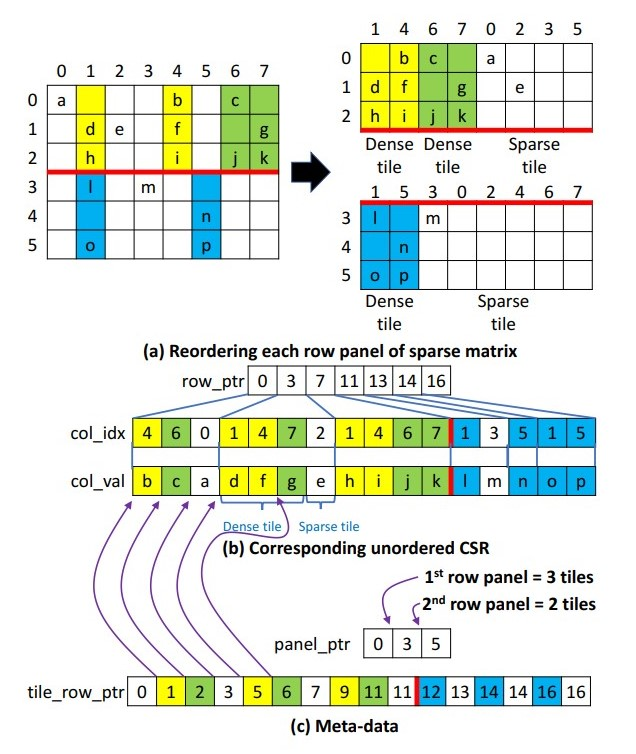
\includegraphics[width=.7\textwidth]{imagenes/chapter3/aspt_csr.jpg}
    \caption{Modificación de CSR con reordenamiento. Extraída de~\cite{Hong2019}.}
    \label{fig:aspt_csr}
\end{figure}
Entonces, la matriz dispersa se divide en paneles de filas, y las columnas activas dentro de cada panel de filas son agrupadas en tiles 2D para la ejecución o se relegan a la ejecución sin \textit{tiling} porque su densidad de columna ``activa'' es inadecuada. La propiedad adaptativa del \textit{tiling} en ASpT viene dada por la combinación el formato CSR con un reordenamiento dentro de las filas, buscando mejorar la localidad de los accesos. Se diferencian de otros autores por utilizar un reordenamiento que no produce tanta sobrecarga como las estrategias clásicas basadas en algoritmos greedy para grafos. Además, la técnica propuesta reordena sólo los elementos no nulos manteniendo una estructura auxiliar y no renumera todo el grafo, es decir, los índices de los elementos para el formato CSR se mantienen. La idea principal es numerar los vértices de modo que a los vértices con muchos vecinos comunes se les asignen índices cercanos entre sí para mejorar la localidad de los accesos. Se puede observar mejor en la Figura~\ref{fig:aspt_csr}.

	% Se carga el capítulo 03
  \chapter{Propuestas}\label{ch:propuestas}

En este capítulo se describen algunas propuestas que buscan incorporar ideas de distintos autores para lograr formatos de almacenamiento más eficientes para clases específicas de matrices dispersas. En particular, la primer parte de este capítulo, Sección~\ref{sec:ae}, está orientada al estudio de heurísticas de reordenamiento utilizando estrategias evolutivas, variando las funciones de evaluación con el objetivo de encontrar nuevos ordenamientos que mejoren la eficiencia de técnicas de compresión de índices como \textit{delta encoding}. Por otra parte, la segunda mitad de éste capítulo, presentada en la Sección~\ref{sec:matrix-cat}, se centra en evaluar y comparar los resultados de combinar estrategias de reordenamiento con formatos de compresión.

% Posterior a la actualización del estado del arte el esfuerzo del proyecto se centró en combinar algunas ideas ya presentadas por autores con el fin de estudiar si pueden ofrecer beneficios extras. En algunos casos también se evalúan estrategias ya abordadas anteriormente pero con una perspectiva más general, es decir, independiente del problema o los casos de estudio para los cuales se utilizan las técnicas en los trabajos originales.

\section*{Casos de estudio}
En el proyecto, se trabaja con matrices de la colección SuiteSparse Matrix Collection \cite{SuiteSparse} %que es la principal colección de matrices dispersas en el campo del ALN. A continuación una breve descripción del la colección basada de : SuiteSparse Matrix Collection 
(anteriormente conocida como University of Florida Sparse Matrix Collection), un conjunto de matrices dispersas que surgen en aplicaciones reales, que continúa en crecimiento. La colección es ampliamente utilizada por la comunidad de álgebra lineal numérica para el desarrollo y evaluación del desempeño de algoritmos para matrices dispersos. Permitiendo a los investigadores realizar experimentos robustos (los resultados de rendimiento con matrices sintéticas generadas artificialmente, pueden ser engañosos) y repetibles (las matrices están disponibles públicamente en los formatos de archivo más comunes)~\cite{SuiteSparse-web}.

% \textit{``The SuiteSparse Matrix Collection (formerly known as the University of Florida Sparse Matrix Collection), is a large and actively growing set of sparse matrices that arise in real applications. The Collection is widely used by the numerical linear algebra community for the development and performance evaluation of sparse matrix algorithms. It allows for robust and repeatable experiments: robust because performance results with artificially-generated matrices can be misleading, and repeatable because matrices are curated and made publicly available in many formats.''}


Este conjunto de matrices cubre un amplio espectro de dominios, divididos en dos grandes grupos. Por un lado, los \textit{Dominios geométricos 2D o 3D}, usualmente provienen de la discretización de EDPs en áreas como ingeniería estructural, dinámica de fluidos computacional, reducción de modelos, etc. Por otro lado, los \textit{Dominios No-Geométricos} corresponden a problemas donde no existe una clara geometría subyacente, como por ejemplo la simulación de procesos químicos, simulación de circuitos, modelado económico y financiero, etc. Estas matrices y la metadata asociadas a cada una, serán accedidas mediante una de las \texttt{API} provistas por el grupo encargado de mantener la colección, en este caso \texttt{MATLAB}.
\begin{figure}[h]
    \centering
    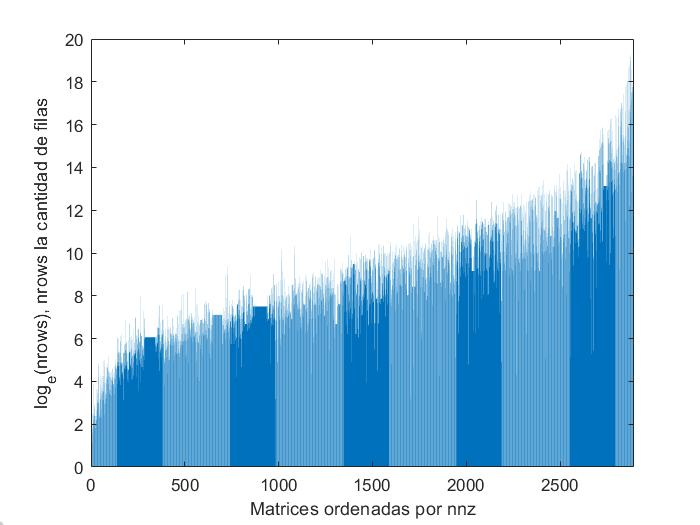
\includegraphics[width=\textwidth]{imagenes/chap4/matrix-sizes.jpg}
    \caption{Cada barra del gráfico simboliza una de las 2893 matrices ordenadas según \textit{nnz}, y su altura la dimensión de la matriz expresada logarítmicamente.}
    \label{fig:matrix-sizes}
\end{figure}
A la fecha, la SSMC está conformada por 2893 matrices de problemas diversos, con múltiples propiedades y patrones. Por ejemplo, 1407 de estas matrices presentan un patrón simétrico, 1185 de éstas tienen además simetría numérica, 601 corresponden a matrices con coeficientes binarios, entre otras posibles categorizaciones\footnote{Notar que algunas de estas clases no son excluyentes entre sí, sino que una matriz puede presentar más de una de estas propiedades}.
A su vez, las matrices pueden ser ordenadas y clasificadas por cantidad de elementos no nulos (\textit{nnz}), así como cantidad de filas y columnas.

Con respecto a la dimensión de los problemas, se pueden encontrar matrices de $2\times 2$ (no tan comunes), hasta aquellas que poseen $226.196.185 \approx e^{19.24}$	filas y columnas, tal y como se puede apreciar en el gráfico de la Figura~\ref{fig:matrix-sizes}. Y en cuanto a la cantidad de elementos no nulos, el valor máximo de \textit{nnz} es $11.588.725.964$, para una matriz de $183.964.077\times183.964.077$.



\section{Reducción de diagonales en matrices}\label{sec:ae}

Como se presentó en la Sección \ref{multiple-precision} algunos autores han utilizado técnicas de reducción del ancho de banda de las matrices para mejorar el uso de formatos de banda o híbridos. 

En un principio, se puso especial foco en la reducción de la cantidad de diagonales, de forma de poder agrupar y representar las diagonales más densas sin la necesidad de utilizar índices para cada elemento no nulo, de manera similar a la planteada en~\cite{Pinar1999} para los bloques. Si una matriz concentra una proporción importante de sus elementos no nulos en posiciones pertenecientes
a unas pocas diagonales densas, se puede dividir la misma  en dos componentes donde uno corresponde a las diagonales densas y el otro al resto de los elementos no nulos.
A continuación se resumen algunos de los esfuerzos realizados en el proyecto en este sentido.


\subsection{Heurísticas para reordenamiento}

Con la idea de verificar y estudiar la posible compresión de matrices, se desarrolla un algoritmo evolutivo capaz de evaluar y encontrar, para la matriz $M$ que se le indique, de tamaño $n \times n$, un vector de permutación $p$ (de tamaño $n$) que, al aplicarlo, minimice lo más que se pueda alguna métrica establecida de antemano, como por ejemplo el ancho de banda de la matriz o la cantidad de diagonales densas. Aplicar la permutación expresada en $p$ a una matriz $M$, implica remplazar cada fila/columna $i$ por la fila/columna $p(i)$. %Que equivalentemente representado por una matriz $P$ se obtiene la matriz $M(p,p) = P\times M \times P^t$, donde las filas y columnas están ordenadas según $p$. 

Los algoritmos evolutivos, buscan soluciones a cierto tipo de problemas sometiendo a una población de individuos a acciones y circunstancias aleatorias semejantes a las que actúan en la evolución biológica (recombinaciones y mutaciones por ejemplo), así como también a una selección de acuerdo con algún criterio, en función del cual se decide cuáles son los individuos más adaptados, que sobreviven, y cuáles los menos aptos, que son descartados. En el Anexo \ref{Ane1} se describen con mayor profundidad los conceptos básicos de estos algoritmos.

En las siguientes sub-secciones se presentan variantes del algoritmo evolutivo en un esfuerzo por encontrar y evidenciar posibles características que presentan las matrices dispersas para explotar formatos basados en diagonales.
En primer lugar, se estudia la posibilidad de reducción de ancho de banda para codificar los enteros de los índices en base a su distancia a la diagonal, buscando ahorrar espacio en el almacenamiento de los mismos. Luego, la idea fue reducir la cantidad de diagonales de las matrices, de forma de poder representar las diagonales más densas sin los índices. Dado que RCM es una heurística con objetivos similares a  estos, porque la reducción del ancho de banda está relacionada muchas veces a la cantidad de diagonales, el estudio se centra en saber si, planteando estos nuevos objetivos, existen soluciones mucho mejores que las dadas por RCM. Por esta razón, se plantean las variantes del algoritmo evolutivo.


\subsubsection{Reducción del ancho de banda}\label{sec:band-reduction-ag}

En este primer caso, con el algoritmo evolutivo se busca evaluar cuán lejos está la permutación generada por RCM de un posible reordenamiento óptimo. En otras palabras, el algoritmo se encargará de obtener, basado en la evaluación del ancho de banda de la matriz en cada iteración, una permutación de filas y columnas capaz de competir con RCM.

%Cuando se habla de un formato diagonal, se hace referencia por ejemplo, al formato DIA (abordado en la Sección \ref{dia-format}), comúnmente utilizado para matrices con anchos de banda reducidos. Parámetro que RCM intenta minimizar, de igual manera el algoritmo evolutivo en esta primer prueba.

El algoritmo diseñado trabaja sobre matrices de tamaño $n \times n$. La familia de individuos o cromosomas serán vectores de permutación de tamaño $n$. La función a minimizar (\textit{fitness}) será el ancho de banda $\beta$ de la matriz. 
Es bien sabido que una componente importante del algoritmo o estrategia evolutiva son los operadores a los cuales se somete a la población de individuos, dado que son la herramienta que permite al algoritmo alcanzar cierta meta u óptimo. 
Para este problema, dado que los genotipos son vectores de permutación, en caso de incluir operadores de cruzamiento (o recombinación) es necesario utilizar estrategias especializadas en este tipo de codificación, quedando excluidos los operadores sencillos como el de un punto de la codificación binaria. Por esta razón, y contemplando el alto costo computacional que implican estos operadores (pruebas preliminares con el operador \textit{Order Crossover}~\cite{AJ2015}) para cruzar estos individuos que presentan restricciones como por ejemplo que no se repitan valores, se decidió no explorar a fondo este camino.
 De forma de intentar reforzar la carencia del operador de cruzamiento, se implementan dos operadores de mutación: \texttt{fliplr} y \texttt{swap}. El primero consiste en invertir el orden de los elementos que componen un individuo, y se aplica a la mitad de los individuos de cada generación, seleccionados aleatoriamente. El segundo operador de mutación, que se aplica con una cierta probabilidad (\textit{Mutation rate}), consiste en realizar un intercambio (\texttt{swap}) entre dos elementos del individuo.

Para la evaluación del algoritmo evolutivo, en las primeras etapas se trabajó con matrices de dimensiones acotadas (y quizás poco representativas). Un ejemplo de estas matrices es \texttt{bfwb62}, correspondiente a un problema  de electromagnetismo, de tamaño $62 \times 62$ y 342 elementos no nulos.
\begin{figure}
\centering
\begin{subfigure}[t]{.3\textwidth}
  \centering
  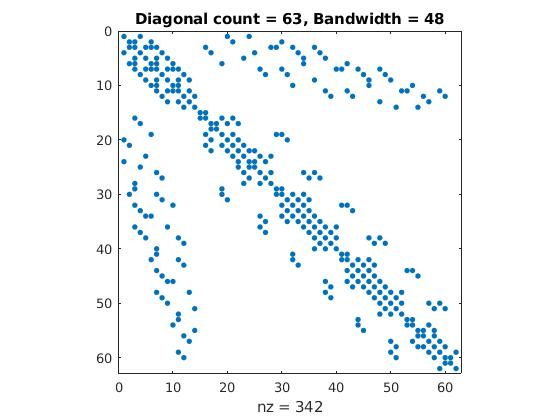
\includegraphics[width=\linewidth]{imagenes/chap4/bfwb62_spy.jpg}
  \caption{bfwb62 original.}
  \label{fig:bfwb62_spy}
\end{subfigure}%
\begin{subfigure}[t]{.3\textwidth}
  \centering
  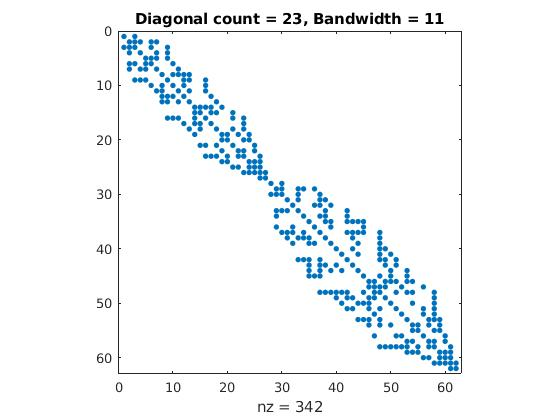
\includegraphics[width=\linewidth]{imagenes/chap4/bfwb62_rcm_spy.jpg}
  \caption{bfwb62 con RCM.}
  \label{fig:bfwb62_rcm_spy}
\end{subfigure}
\begin{subfigure}[t]{.3\textwidth}
  \centering
  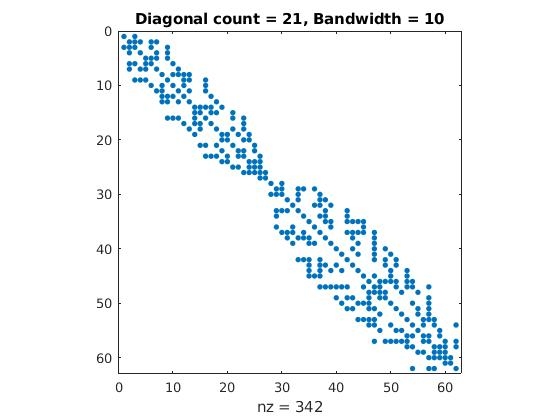
\includegraphics[width=\linewidth]{imagenes/chap4/bfwb62_ga_band_spy.jpg}
  \caption{bfwb62 con el algoritmo evolutivo.}
  \label{fig:bfwb62_ga_spy}
\end{subfigure}
\caption{Tres estados de la matriz \texttt{bfwb62} con diferentes reordenamientos.}
\label{fig:bfwb62_band}
\end{figure}
En la Figura~\ref{fig:bfwb62_band} se muestran tres instancias de la matriz con reordenamientos distintos. Pese a que las imágenes no muestran una diferencia significativa, principalmente entre RCM y la estrategia evolutiva, aplicando la permutación obtenida con el algoritmo evolutivo, se logra reducir en un elemento el ancho de banda con respecto al reordenamiento generado por RCM. 

\subsubsection*{Evaluación experimental}

El resto de las pruebas se realizaron sobre un subconjunto de matrices de problemas variados y con patrones distintos, buscando cierta heterogeneidad en las pruebas. En general, la dimensión de estas matrices es solo ligeramente mayor que la de la prueba anterior, debido a la creciente cantidad de cómputo necesaria que va a la par con la dimensión de los problemas.

Para las pruebas, el arreglo de los parámetros con los que se instanció el algoritmo evolutivo son los siguientes :
\begin{itemize}
    \item Población inicial: 240 individuos
    divididos en tres grupos, una porción de individuos o permutaciones correspondiente a la identidad, es decir, un vector que contiene de forma ordenada los valores de 1 a $n$, siendo $n$ la dimensión de la matriz, otra porción de individuos con la permutación obtenida de aplicar RCM, y el resto, la porción más grande, de permutaciones aleatorias.
    \item \textit{Generations} o cantidad máxima de generaciones: 2500,
    \item \textit{Mutation rate} o probabilidad de mutación: $0,2$,
    \item \textit{Operadores:} los dos operadores de mutación antes mencionados.
\end{itemize}

\begin{table}[h]
\resizebox{\textwidth}{!}{
\begin{tabular}{|l|r|r|r|r|r|r|r|r|r|r|r|} 
\hline
\multirow{2}{*}{\textbf{ Matriz}} & \multicolumn{1}{l|}{\multirow{2}{*}{\textbf{ Dim($n$)}}} & \multicolumn{1}{l|}{\multirow{2}{*}{\textbf{ \nnz}}} & \multicolumn{2}{c|}{\textbf{Original}}            & \multicolumn{2}{c|}{\textbf{RCM}}                 & \multicolumn{2}{c|}{\textbf{AE}}                  & \multicolumn{3}{c|}{\textbf{\bw reduction (\%)}}                                           \\ 
\cline{4-12}
                                  & \multicolumn{1}{l|}{}                                   & \multicolumn{1}{l|}{}                               & \multicolumn{1}{l|}{\dc} & \multicolumn{1}{l|}{\bw} & \multicolumn{1}{l|}{\dc} & \multicolumn{1}{l|}{\bw} & \multicolumn{1}{l|}{\dc} & \multicolumn{1}{l|}{\bw} & \multicolumn{1}{l|}{RCM - Orig.} & \multicolumn{1}{l|}{AE - Orig.} & \multicolumn{1}{l|}{AE - RCM}  \\ 
\hline \hline
'662\_bus'                    & 662                                                     & 2474                                                & 463                     & 335                     & 237                     & 118                     & 237                     & 118                     & 64.78\%                             & 64.78\%                            & 0.00\%                         \\ 
\hline
'S10PI\_n1'                   & 528                                                     & 1317                                                & 97                      & 509                     & 29                      & 14                      & 27                      & 13                      & 97.25\%                             & 97.45\%                            & 7.14\%                         \\ 
\hline
'Si2'                         & 769                                                     & 17801                                               & 1013                    & 552                     & 649                     & 324                     & 649                     & 324                     & 41.30\%                             & 41.30\%                            & 0.00\%                         \\ 
\hline
'Spectro\_10NN'               & 531                                                     & 7422                                                & 994                     & 518                     & 192                     & 96                      & 190                     & 95                      & 81.47\%                             & 81.66\%                            & 1.04\%                         \\ 
\hline
'Trefethen\_700'              & 700                                                     & 12654                                               & 21                      & 512                     & 655                     & 327                     & 655                     & 327                     & 36.13\%                             & 36.13\%                            & 0.00\%                         \\ 
\hline
'bfwb782'                     & 782                                                     & 5982                                                & 593                     & 593                     & 71                      & 35                      & 71                      & 35                      & 94.10\%                             & 94.10\%                            & 0.00\%                         \\ 
\hline
'dendrimer'                   & 730                                                     & 63024                                               & 1355                    & 708                     & 853                     & 426                     & 835                     & 417                     & 39.83\%                             & 41.10\%                            & 2.11\%                         \\ 
\hline
'dwt\_503'                    & 503                                                     & 6027                                                & 477                     & 452                     & 129                     & 64                      & 129                     & 64                      & 85.84\%                             & 85.84\%                            & 0.00\%                         \\ 
\hline
'goddardRocket'     & 831                                                     & 8498                                                & 723                     & 777                     & 575                     & 287                     & 573                     & 286                     & 63.06\%                             & 63.19\%                            & 0.35\%                         \\ 
\hline
'lowThrust\_1'                & 584                                                     & 6133                                                & 509                     & 487                     & 607                     & 303                     & 595                     & 297                     & 37.78\%                             & 39.01\%                            & 1.98\%                         \\ 
\hline
'lshp\_577'                   & 577                                                     & 3889                                                & 325                     & 563                     & 53                      & 26                      & 53                      & 26                      & 95.38\%                             & 95.38\%                            & 0.00\%                         \\ 
\hline
'lshp\_778'                   & 778                                                     & 5272                                                & 411                     & 762                     & 61                      & 30                      & 61                      & 30                      & 96.06\%                             & 96.06\%                            & 0.00\%                         \\ 
\hline
'nos6'                        & 675                                                     & 3255                                                & 7                       & 30                      & 33                      & 16                      & 33                      & 16                      & 46.67\%                             & 46.67\%                            & 0.00\%                         \\ 
\hline
'orsirr\_2'                   & 886                                                     & 5970                                                & 437                     & 554                     & 245                     & 122                     & 245                     & 122                     & 77.98\%                             & 77.98\%                            & 0.00\%                         \\ 
\hline
'steam2'                      & 600                                                     & 5660                                                & 123                     & 330                     & 152                     & 76                      & 152                     & 76                      & 76.97\%                             & 76.97\%                            & 0.00\%                         \\ 
\hline
'young4c'                     & 841                                                     & 4089                                                & 5                       & 29                      & 59                      & 29                      & 59                      & 29                      & 0.00\%                              & 0.00\%                             & 0.00\%                         \\
\hline
\end{tabular}
}
\caption{Resultados del algoritmo evolutivo intentando minimizar el \textit{bandwidth} sobre el subconjunto de matrices.}
\label{tab:band-reduction-ag-results}
\end{table}

Los resultados de la evaluación se presentan en la Tabla~\ref{tab:band-reduction-ag-results}, dónde cada fila corresponde a los resultados para cada matriz, medidos o cuantificados con los parámetros: \textit{bandwidth} (\bw) y \textit{diagonal count} (\dc). Para el análisis se pondrá foco, principalmente, en las columnas porcentuales. La columna RCM-Orig. corresponde al porcentaje de reducción de ancho de banda luego de aplicar el reordenamiento generado por RCM, comparado con la matriz original. De manera similar se presenta en la columna AE-Orig., dónde se muestran los porcentajes de reducción obtenidos por el algoritmo evolutivo con respecto al reordenamiento original. Y una columna interesante es la última, AE-RCM, que muestra el porcentaje de reducción del algoritmo evolutivo comparado con el ordenamiento de RCM. De esta tabla se puede observar que, en general, los valores de ancho de banda obtenidos con el algoritmo evolutivo no se alejaron mucho de los obtenidos mediante reordenamientos generados por la heurística RCM. Son pocos los casos en que el algoritmo logró una permutación con mejor ancho de banda que RCM y, en particular, la mejora ronda en el 1\%. Siendo, posiblemente, un indicador de que los reordenamientos obtenidos con RCM son más que aceptables, dado su razonable costo computacional y midiendo la eficacia de éste según el ancho de banda resultante. 



\subsubsection{Reducción de la cantidad de diagonales}\label{sec:diag-reduction-ag}

En esta segunda prueba para el algoritmo evolutivo, lo que se busca, es obtener permutaciones que logren reducir significativamente la cantidad de diagonales independientemente de si el ancho de banda (bandwidth) se ve optimizado o no.

Naturalmente, para este nuevo enfoque es necesaria la modificación de la función \textit{fitness}, que para este caso se corresponderá con la cantidad de diagonales luego de permutar la matriz. El resto de los aspectos del algoritmo se mantienen incambiados.

\subsubsection*{Evaluación experimental}

% Para la evaluación del algoritmo evolutivo, en las primeras etapas se trabajó con matrices de dimensiones acotadas (y quizás poco representativas). Un ejemplo de estas matrices: \texttt{bfwb62}, correspondiente a un problema  de electromagnetismo, de tamaño $62 \times 62$ y 342 elementos no nulos.
Siguiendo la metodología de evaluación utilizada en la Sección~\ref{sec:band-reduction-ag} se hizo una prueba de concepto con la matriz \texttt{bfwb62}. En la Figura~\ref{fig:bfwb62-diag}, se puede observar una mejora significativa con respecto a su ordenamiento original y el de RCM. Comparado con RCM, se logra reducir en aproximadamente 21\% la cantidad de diagonales. Incluso sin que ese sea el objetivo, se produce también una reducción en el ancho de banda, logrando una reducción de 18\% con respecto a RCM, mejor resultado que el obtenido por el algoritmo en la Sección~\ref{sec:band-reduction-ag}.

% \begin{figure}[]
%   \centering
%   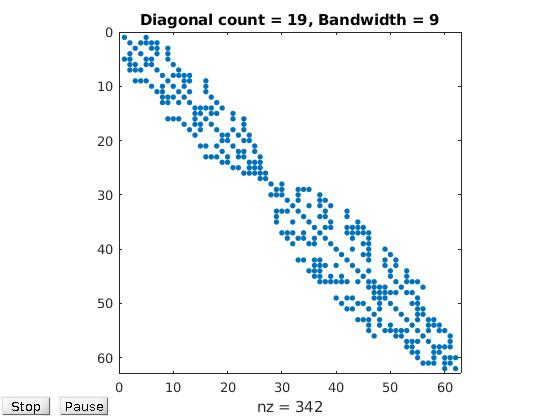
\includegraphics[width=.3\textwidth]{imagenes/chap4/bfwb62_ga_spy.jpg}
%   \caption{\texttt{bfwb62} con el algoritmo evolutivo.}
%   \label{fig:bfwb62_diag_ga_spy}
% \end{figure}

\begin{figure}
\centering
\begin{subfigure}[t]{.3\textwidth}
  \centering
  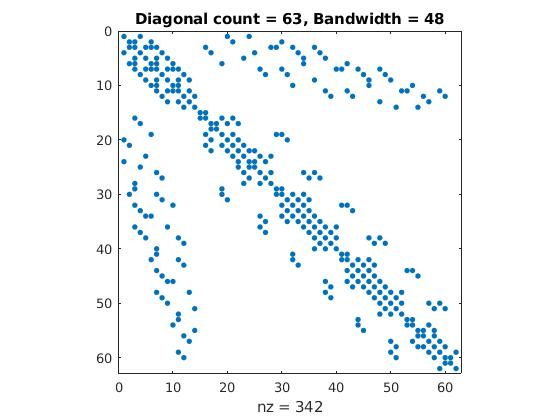
\includegraphics[width=\linewidth]{imagenes/chap4/bfwb62_spy.jpg}
  \caption{bfwb62 original.}
  \label{fig:bfwb62_spy-diag}
\end{subfigure}%
\begin{subfigure}[t]{.3\textwidth}
  \centering
  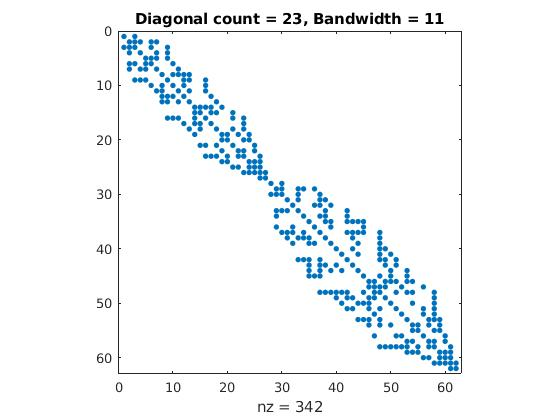
\includegraphics[width=\linewidth]{imagenes/chap4/bfwb62_rcm_spy.jpg}
  \caption{bfwb62 con RCM.}
  \label{fig:bfwb62_rcm_spy-diag}
\end{subfigure}
\begin{subfigure}[t]{.3\textwidth}
  \centering
  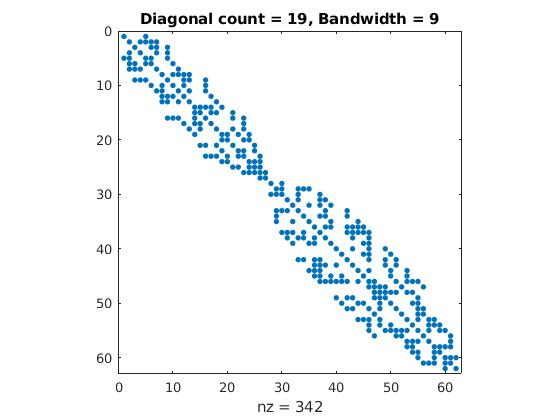
\includegraphics[width=\linewidth]{imagenes/chap4/bfwb62_ga_spy_.jpg}
  \caption{bfwb62 con el algoritmo evolutivo.}
  \label{fig:bfwb62_ga_spy-diag}
\end{subfigure}
\caption{Tres estados de la matriz \texttt{bfwb62} con diferentes reordenamientos.}
\label{fig:bfwb62-diag}
\end{figure}

% De la Figura~\ref{fig:bfwb62} se muestran tres instancias de la matriz con reordenamientos distintos. La idea es poder comparar y discutir la validez del reordenamiento obtenido con el algoritmo evolutivo. De las figuras se desprende que aplicando la permutación obtenida con el algoritmo evolutivo, se logra reducir en aproximadamente $21\%$ la cantidad de diagonales, con respecto al reordenamiento generado por RCM. 


En la etapa de evaluación de esta segunda versión de la estrategia evolutiva, se utilizó el mismo conjunto de  matrices, con la idea de obtener resultados comparativos entre los dos enfoques. Los parámetros del algoritmo, a excepción de la función de \textit{fitness} (en este caso cuenta la cantidad de diagonales), se mantienen.

Los resultados de las pruebas se pueden observar en la Tabla~\ref{tab:diag-reduction-ag-results}, análoga a la presentada en el apartado de evaluación de la Sección~\ref{sec:band-reduction-ag}.


\begin{table}[h]
\centering
\resizebox{\textwidth}{!}{
\begin{tabular}{|l|r|r|r|r|r|r|r|r|r|r|r|} 
\hline
\multirow{2}{*}{\textbf{ Matriz}} & \multicolumn{1}{l|}{\multirow{2}{*}{\textbf{ Dim($n$)}}} & \multicolumn{1}{l|}{\multirow{2}{*}{\textbf{ \nnz}}} & \multicolumn{2}{c|}{\textbf{Original}}            & \multicolumn{2}{c|}{\textbf{RCM}}                 & \multicolumn{2}{c|}{\textbf{AE}}                  & \multicolumn{3}{c|}{\textbf{\dc reduction (\%)}}                                                           \\ 
\cline{4-12}
                                  & \multicolumn{1}{l|}{}                                   & \multicolumn{1}{l|}{}                               & \multicolumn{1}{l|}{\dc} & \multicolumn{1}{l|}{\bw} & \multicolumn{1}{l|}{\dc} & \multicolumn{1}{l|}{\bw} & \multicolumn{1}{l|}{\dc} & \multicolumn{1}{l|}{\bw} & \multicolumn{1}{l|}{RCM - Orig.} & \multicolumn{1}{l|}{AE - Orig.} & \multicolumn{1}{l|}{AE - RCM}  \\ 
\hline\hline
'662\_bus'                    & 662                                                     & 2474                                                & 463                     & 335                     & 237                     & 118                     & 205                     & 118                     & 48.81\%                             & 55.72\%                            & 13.50\%                        \\ 
\hline
'S10PI\_n1'                   & 528                                                     & 1317                                                & 97                      & 509                     & 29                      & 14                      & 27                      & 13                      & 70.10\%                             & 72.16\%                            & 6.90\%                         \\ 
\hline
'Si2'                         & 769                                                     & 17801                                               & 1013                    & 552                     & 649                     & 324                     & 649                     & 324                     & 35.93\%                             & 35.93\%                            & 0.00\%                         \\ 
\hline
'Spectro\_10NN'               & 531                                                     & 7422                                                & 994                     & 518                     & 192                     & 96                      & 190                     & 95                      & 80.68\%                             & 80.89\%                            & 1.04\%                         \\ 
\hline
'Trefethen\_700'              & 700                                                     & 12654                                               & 21                      & 512                     & 655                     & 327                     & 21                      & 512                     & -3019.05\%                          & 0.00\%                             & 96.79\%                        \\ 
\hline
'bfwb782'                     & 782                                                     & 5982                                                & 593                     & 593                     & 71                      & 35                      & 71                      & 35                      & 88.03\%                             & 88.03\%                            & 0.00\%                         \\ 
\hline
'dendrimer'                   & 730                                                     & 63024                                               & 1355                    & 708                     & 853                     & 426                     & 773                     & 386                     & 37.05\%                             & 42.95\%                            & 9.38\%                         \\ 
\hline
'dwt\_503'                    & 503                                                     & 6027                                                & 477                     & 452                     & 129                     & 64                      & 129                     & 64                      & 72.96\%                             & 72.96\%                            & 0.00\%                         \\ 
\hline
'goddardRocket'     & 831                                                     & 8498                                                & 723                     & 777                     & 575                     & 287                     & 465                     & 324                     & 20.47\%                             & 35.68\%                            & 19.13\%                        \\ 
\hline
'lowThrust\_1'                & 584                                                     & 6133                                                & 509                     & 487                     & 607                     & 303                     & 427                     & 468                     & -19.25\%                            & 16.11\%                            & 29.65\%                        \\ 
\hline
'lshp\_577'                   & 577                                                     & 3889                                                & 325                     & 563                     & 53                      & 26                      & 53                      & 26                      & 83.69\%                             & 83.69\%                            & 0.00\%                         \\ 
\hline
'lshp\_778'                   & 778                                                     & 5272                                                & 411                     & 762                     & 61                      & 30                      & 61                      & 30                      & 85.16\%                             & 85.16\%                            & 0.00\%                         \\ 
\hline
'nos6'                        & 675                                                     & 3255                                                & 7                       & 30                      & 33                      & 16                      & 7                       & 30                      & -371.43\%                           & 0.00\%                             & 78.79\%                        \\ 
\hline
'orsirr\_2'                   & 886                                                     & 5970                                                & 437                     & 554                     & 245                     & 122                     & 245                     & 122                     & 43.94\%                             & 43.94\%                            & 0.00\%                         \\ 
\hline
'steam2'                      & 600                                                     & 5660                                                & 123                     & 330                     & 152                     & 76                      & 123                     & 330                     & -23.58\%                            & 0.00\%                             & 19.08\%                        \\ 
\hline
'young4c'                     & 841                                                     & 4089                                                & 5                       & 29                      & 59                      & 29                      & 5                       & 29                      & -1080.00\%                          & 0.00\%                             & 91.53\%                        \\
\hline
\end{tabular}
}
\caption{Resultados del algoritmo evolutivo intentando minimizar la cantidad de diagonales sobre sobre el subconjunto de matrices.}
\label{tab:diag-reduction-ag-results}
\end{table}



Dado que el conjunto de matrices fue elegido de modo que las mismas presenten características heterogéneas, los resultados se pueden dividir en tres grupos.
El primero de ellos, son aquellas matrices que originalmente presentan un mejor ordenamiento que el que puede generar RCM (en algunos casos tanto para cantidad de diagonales como ancho de banda). En estos casos posiblemente el ordenamiento original sea el óptimo, por lo que el algoritmo evolutivo tiende a quedarse con dicho ordenamiento original. Por ejemplo, observar las filas de la Tabla~\ref{tab:diag-reduction-ag-results} correspondientes a las matrices \texttt{Trefethen\_700} y \texttt{nos6}. 
Como segundo caso, están aquellas matrices para las cuales RCM obtiene una muy buena permutación, por ejemplo, \texttt{lshp\_577}, \texttt{lshp\_778} y \texttt{dwt503}. El efecto del algoritmo evolutivo para estos casos, es similar producido en el experimento anterior no logrando mejoras sustanciales con respecto a la solución obtenida con RCM. Observar los resultados de 0\% en la columna AE-RCM.
Y el tercer caso, el que presenta mayor interés, son aquellas que permiten evidenciar cuán lejos está RCM de un posible óptimo. Entonces, para analizar más en detalle los resultados, se centran los esfuerzos de la discusión sobre el tercer conjunto. 

De las pruebas realizadas, se puede observar que para 4 de 6 matrices para las cuales el algoritmo presenta un mejor reordenamiento que el de RCM y el original, el algoritmo evolutivo obtiene soluciones que lo sobrepasan a RCM por aproximadamente 10\%. Hay incluso, un caso donde se logra una mejora de un 29\% con respecto a RCM, y es para la matriz \texttt{lowThrust1}, donde RCM obtuvo un mal rendimiento medido en cantidad de diagonales.

En general, cuando RCM obtiene una permutación que no favorece en la cantidad de  diagonales, es decir, aumenta significativamente este valor, el resultado obtenido por el algoritmo tiende a ser similar al ordenamiento original. % (Es mas del primer caso creo...)

% matrices admiten un reordenamiento de alrededor del 10\% mejor que el generado por RCM, medido en cantidad de diagonales.


%conjunto utilizado en numerosas investigaciones para evaluar nuevas propuestas a modo de benchmark, principalmente para nuevos formatos dispersos que buscan mejorar la o SpMV~\cite{Maggioni2014,Xu2010, Bell2009, GarlandAndBell2009} (casi seguro que hay mas). (Hasta ahora, las pruebas no han salido bien, no se mueve ninguna de las cantidades para estas matrices grandes).

\subsubsection{Cantidad fija de diagonales para formatos híbridos}\label{sec:diag-perc-reduction}

Habiendo estudiado la posibilidad de reordenar las matrices intentando reducir ancho de banda y cantidad de diagonales, con un enfoque en la posible aplicación de formatos de compresión de índices%utilizando \textit{delta encoding}, como formatos de banda que almacenan la matriz por sus diagonales
, a continuación se plantea un estudio del mismo conjunto de matrices, ahora con el objetivo de emplear formatos híbridos (por ejemplo HYB, entre otros). En este caso se almacena la matriz, generalmente, en dos partes, una con una estructura razonablemente regular y la otra completamente dispersa. Modificando el algoritmo evolutivo, se intenta encontrar la permutación que, aplicada a las matrices, maximice la cantidad de elementos no nulos en cierta cantidad fija de diagonales, sin intentar optimizar el resto de parámetros. Es decir, se busca lograr una permutación que genere algunas diagonales densas (posiblemente cerca de la diagonal principal), de forma de poder almacenar las mismas en una estructura regular, en lugar de minimizar el ancho de banda y cantidad de diagonales. Notar que esta estrategia tiene cierto límite. En una matriz de tamaño $n\times n$, en el mejor de los casos, si se logra disponer los elementos en las $d$ diagonales que son más próximas a la principal, igualmente puede suceder que la cantidad de elementos no nulos de la matriz sea mayor a las entradas disponibles para $d$ diagonales. Cabe destacar que, para la evaluación, no se tomó en consideración que los elementos no nulos estuviesen en dichas diagonales próximas a la principal, sino que se calcula entre todas, la cantidad de elementos que cada una posee y posteriormente se selecciona aquellas $d$ con mayor cantidad de \textit{nnz}. 

\subsubsection*{Evaluación experimental}

Para la evaluación de esta estrategia, con respecto a las anteriores sólo cambia la función \textit{fitness}. Ahora en lugar de minimizar, como se realizó para los parámetros elegidos en las Secciones~\ref{sec:band-reduction-ag}~y~\ref{sec:diag-reduction-ag}, la función calcula la máxima cantidad de elementos no nulos en una cantidad fija de diagonales $d$, expresada en la implementación como un porcentaje de $n$. 
Para estas pruebas, el porcentaje de diagonales fue un 2\% de $n$. 
% $d = round(n/100)\times 2$, valor que depende de las dimensiones de cada matriz.

\begin{table}[]
\centering
\resizebox{\textwidth}{!}{
\begin{tabular}{|l|r|r|r|r|r|r|r|r|r|r|r|r|r|r|r|} 
\hline
\multirow{2}{*}{\textbf{Matriz}} & \multicolumn{1}{l|}{\multirow{2}{*}{\begin{tabular}[c]{@{}l@{}}\textbf{Dim} \\ \textbf{($n$)}\end{tabular}}} & \multicolumn{1}{l|}{\multirow{2}{*}{\textbf{\nnz}}} & \multicolumn{1}{l|}{\multirow{2}{*}{\begin{tabular}[c]{@{}l@{}}\textbf{2\%} \\ \textbf{DIAG}\end{tabular}}} & \multicolumn{4}{c|}{\textbf{Original}}                                                                                                                                                                               & \multicolumn{4}{c|}{\textbf{RCM}}                                                                                                                                                                                     & \multicolumn{4}{c|}{\textbf{AE}}                                                                                                                                                                                       \\ 
\cline{5-16}
                                  & \multicolumn{1}{l|}{}                                   & \multicolumn{1}{l|}{}                               & \multicolumn{1}{l|}{}                                    & \multicolumn{1}{l|}{\dc} & \multicolumn{1}{l|}{\bw} & \multicolumn{1}{l|}{\begin{tabular}[c]{@{}l@{}}NNZ IN \\2\% DIAG\end{tabular}} & \multicolumn{1}{l|}{\begin{tabular}[c]{@{}l@{}}\%NNZ IN\\ 2\%~DIAG\end{tabular}} & \multicolumn{1}{l|}{\dc} & \multicolumn{1}{l|}{\bw} & \multicolumn{1}{l|}{\begin{tabular}[c]{@{}l@{}}NNZ IN\\             2\% DIAG\end{tabular}} & \multicolumn{1}{l|}{\begin{tabular}[c]{@{}l@{}}\%NNZ IN             \\2\% DIAG\end{tabular}} & \multicolumn{1}{l|}{\dc} & \multicolumn{1}{l|}{\bw} & \multicolumn{1}{l|}{\begin{tabular}[c]{@{}l@{}}NNZ IN \\            2\% DIAG\end{tabular}} & \multicolumn{1}{l|}{\begin{tabular}[c]{@{}l@{}}\%NNZ IN             \\2\% DIAG\end{tabular}}  \\ 
\hline \hline
'662\_bus'                    & 662                                                     & 2474                                                & 14                                                       & 463                     & 335                     & 951                                                                           & 38.44\%                                                                          & 237                     & 118                     & 966                                                                            & 39.05\%                                                                          & 529                     & 651                     & 1701                                                                           & 68.76\%                                                                           \\ 
\hline
'S10PI\_n1'                   & 528                                                     & 1317                                                & 10                                                       & 97                      & 509                     & 1223                                                                          & 92.86\%                                                                          & 29                      & 14                      & 1058                                                                           & 80.33\%                                                                          & 65                      & 513                     & 1256                                                                           & 95.37\%                                                                           \\ 
\hline
'Si2'                         & 769                                                     & 17801                                               & 16                                                       & 1013                    & 552                     & 7029                                                                          & 39.49\%                                                                          & 649                     & 324                     & 4256                                                                           & 23.91\%                                                                          & 1099                    & 768                     & 7200                                                                           & 40.45\%                                                                           \\ 
\hline
'Spectro\_10NN'               & 531                                                     & 7422                                                & 10                                                       & 994                     & 518                     & 208                                                                           & 2.80\%                                                                           & 192                     & 96                      & 2182                                                                           & 29.40\%                                                                          & 340                     & 530                     & 3130                                                                           & 42.17\%                                                                           \\ 
\hline
'Trefethen\_700'              & 700                                                     & 12654                                               & 14                                                       & 21                      & 512                     & 9610                                                                          & 75.94\%                                                                          & 655                     & 327                     & 2818                                                                           & 22.27\%                                                                          & 21                      & 512                     & 9610                                                                           & 75.94\%                                                                           \\ 
\hline
'bfwb62'                      & 62                                                      & 342                                                 & 2                                                        & 63                      & 48                      & 94                                                                            & 27.49\%                                                                          & 23                      & 11                      & 86                                                                             & 25.15\%                                                                          & 83                      & 60                      & 108                                                                            & 31.58\%                                                                           \\ 
\hline
'bfwb782'                     & 782                                                     & 5982                                                & 16                                                       & 593                     & 593                     & 3733                                                                          & 62.40\%                                                                          & 71                      & 35                      & 2926                                                                           & 48.91\%                                                                          & 609                     & 597                     & 3785                                                                           & 63.27\%                                                                           \\ 
\hline
'dendrimer'                   & 730                                                     & 63024                                               & 14                                                       & 1355                    & 708                     & 8000                                                                          & 12.69\%                                                                          & 853                     & 426                     & 4551                                                                           & 7.22\%                                                                           & 1425                    & 729                     & 9168                                                                           & 14.55\%                                                                           \\ 
\hline
'dwt\_503'                    & 503                                                     & 6027                                                & 10                                                       & 477                     & 452                     & 2190                                                                          & 36.34\%                                                                          & 129                     & 64                      & 1919                                                                           & 31.84\%                                                                          & 537                     & 493                     & 2813                                                                           & 46.67\%                                                                           \\ 
\hline
'goddardRocket'     & 831                                                     & 8498                                                & 16                                                       & 723                     & 777                     & 2937                                                                          & 34.56\%                                                                          & 575                     & 287                     & 1472                                                                           & 17.32\%                                                                          & 727                     & 789                     & 4291                                                                           & 50.49\%                                                                           \\ 
\hline
'lowThrust\_1'                & 584                                                     & 6133                                                & 12                                                       & 509                     & 487                     & 2377                                                                          & 38.76\%                                                                          & 607                     & 303                     & 836                                                                            & 13.63\%                                                                          & 721                     & 547                     & 2554                                                                           & 41.64\%                                                                           \\ 
\hline
'lshp\_577'                   & 577                                                     & 3889                                                & 12                                                       & 325                     & 563                     & 2487                                                                          & 63.95\%                                                                          & 53                      & 26                      & 2680                                                                           & 68.91\%                                                                          & 277                     & 571                     & 3072                                                                           & 78.99\%                                                                           \\ 
\hline
'lshp\_778'                   & 778                                                     & 5272                                                & 16                                                       & 411                     & 762                     & 3583                                                                          & 67.96\%                                                                          & 61                      & 30                      & 3920                                                                           & 74.36\%                                                                          & 355                     & 766                     & 4310                                                                           & 81.75\%                                                                           \\ 
\hline
'nos6'                        & 675                                                     & 3255                                                & 14                                                       & 7                       & 30                      & 3255                                                                          & 100.00\%                                                                         & 33                      & 16                      & 2893                                                                           & 88.88\%                                                                          & 7                       & 30                      & 3255                                                                           & 100.00\%                                                                          \\ 
\hline
'orsirr\_2'                   & 886                                                     & 5970                                                & 18                                                       & 437                     & 554                     & 5170                                                                          & 86.60\%                                                                          & 245                     & 122                     & 2491                                                                           & 41.73\%                                                                          & 437                     & 554                     & 5170                                                                           & 86.60\%                                                                           \\ 
\hline
'steam2'                      & 600                                                     & 5660                                                & 12                                                       & 123                     & 330                     & 2413                                                                          & 42.63\%                                                                          & 152                     & 76                      & 2116                                                                           & 37.39\%                                                                          & 230                     & 595                     & 2518                                                                           & 44.49\%                                                                           \\ 
\hline
'young4c'                     & 841                                                     & 4089                                                & 16                                                       & 5                       & 29                      & 4089                                                                          & 100.00\%                                                                         & 59                      & 29                      & 2295                                                                           & 56.13\%                                                                          & 5                       & 29                      & 4089                                                                           & 100.00\%                                                                          \\
\hline
\end{tabular}
}
\caption{Resultados del algoritmo evolutivo intentando maximizar la cantidad de elementos no nulos en $d$ diagonales para cada matriz del subconjunto de matrices.}
\label{tab:max-nnz-diag-ag-results}
\end{table}

% Algunas observaciones de los resultados presentados en la Tabla~\ref{tab:max-nnz-diag-ag-results} son los siguientes: en general RCM, para las pruebas realizadas, si bien existen casos donde se logran mejora, tiende a empeorar la cantidad de elementos no nulos que van a parar en una cantidad de diagonales fija $d$ con respecto a la matriz original.
La Tabla~\ref{tab:max-nnz-diag-ag-results} muestra que, luego de aplicar los ordenamientos, RCM tiende a disminuir la cantidad de elementos no nulos en las $d$ diagonales más próximas a la principal.
Por este motivo, se hace especial foco en comparar los resultados del algoritmo evolutivo con el ordenamiento original que presentan las matrices. En general, se puede apreciar que hay una aparente mejora de unos pocos puntos porcentuales por parte del algoritmo evolutivo. También se pueden observar casos en los que no se la logra maximizar la cantidad de elementos no nulos en las $d$  diagonales en absoluto, indicando posiblemente que son matrices con estructuras diagonales, como es el caso de \texttt{nos6}, que tiene un patrón bien definido. Para 5 matrices en las que el reordenamiento original supera al de RCM, el algoritmo evolutivo logra aumentar un 3\% la cantidad de elementos no nulos alrededor de la diagonal principal. Para otras 4 matrices del conjunto de prueba, la mejora fue de un 14\%. Como máximos resultados de optimización, a 2 matrices se las logra optimizar en un 30.3\% y 39.4\%.

% En general creo que esperabamos resultados mejores, ahora voy a dejar otra corrida, no se, me parecio que estaba dejando mejores resultados...

\subsection{Resumen de los resultados obtenidos}

% \resumen{Pensaba agregar esta sección para discutir y comparar los resultados de las tres estrategias aplicadas con la estrategia evolutiva}

Observando las Tablas \ref{tab:band-reduction-ag-results} y \ref{tab:diag-reduction-ag-results}, es bastante claro cómo, al utilizar la cantidad de diagonales como función \textit{fitness}, los resultados obtenidos fueron mejores que con la estrategia del \textit{bandwidth}. Cabe destacar que, % medido no sólo según la función \textit{fitness} en cada instancia del algoritmo, sino que 
en algunos casos, %de la prueba de la Sección~\ref{sec:diag-reduction-ag} se puede apreciar que 
la reducción de diagonales también implicó una reducción del ancho de banda, obteniendo mejores resultados que en el algoritmo que emplea el ancho de banda como función \textit{fitness}. Si bien ambas estrategias no son eficientes comparadas con la mayoría de las heurísticas de reordenamiento para la reducción del ancho de banda, los resultados podrían evidenciar que quizás, en lugar de enfocar los esfuerzos en reducir directamente el ancho de banda, podría ser una mejor estrategia enfocarse en reducir la cantidad de diagonales.

Con respecto a la última idea evaluada, si bien RCM en los anteriores casos resultó ser un buen comienzo para el espacio de búsqueda de un reordenamiento opitmizado, como se puede observar en la Tabla~\ref{tab:max-nnz-diag-ag-results} este no es el caso. Esto debido, probablemente, a la naturaleza del RCM no enfocado en directamente en lograr la menor cantidad de diagonales densas posibles.


\section{Categorización de matrices (Estudio del espacio de matrices)}\label{sec:matrix-cat}

Para evaluar que tan efectivas podrían ser las técnicas de compresión de matrices dispersas basadas en la reducción de precisión para almacenar los índices, a continuación se presenta una clasificación o categorización de un gran grupo de matrices de \texttt{SuiteSparse Matrix Collection}. En particular, las matrices de la colección que son simétricas, a las que se les puede aplicar técnicas de reordenamiento para reducir su ancho de banda. Se evalúa para las matrices mencionadas, utilizando técnicas distintas, cuál es la cantidad de bits mínima con la que se podría almacenar las coordenadas si se utiliza otro valor como índice de columna. Entre las estrategias que se evalúan están, reducir la precisión de los índices actuales basados en las dimensiones de la matriz, sustituir el índice por la distancia a la diagonal, y por último utilizar la diferencia con el elemento no nulo anterior o \textit{delta encoding}.

Para esta tarea se programaron rutinas (scripts y funciones) en \texttt{MATLAB}, que accediendo a través de la \texttt{API} de SSMC obtienen las matrices simétricas, y aplican las técnicas que se describen en las siguientes secciones. 


% Posteriormente, obtenidas estas matrices permutadas y a sus correspondientes originales, se procede en la obtención de datos, calculando por ejemplo anchos de banda por filas, almacenando en el proceso parámetros de interés como son: cantidad de filas representables en diferentes precisiones, distancia máxima entre elementos no nulos consecutivos, entre otros. Obtenidos los datos, se estudian para tres rangos distintos, cuantas de las filas de cada matriz pueden ser representadas si los índices se expresan como enteros en 8, 16 y 32 bits\footnote{Notar que para el caso de diferencia a la diagonal, se necesitan representaciones de enteros con signo.}. Dando como resultados los rangos $[-2^7,2^7]$, $[-2^{15},2^{15}]$ y $[-2^{31},2^{31}]$ para el caso de la diferencia a la diagonal y  los rangos $[0,2^8 - 1]$, $[0,2^{16} - 1]$ y $[0,2^{32} - 1]$ respectivamente para el caso de la diferencia con el elemento no nulo anterior.

\subsection{Comprimir los índices de cada fila sin modificarlos}\label{col-index-compression}

El primer estudio planteado consistió en evaluar la capacidad de compresión al utilizar los índices originales asociados %a cada elemento directamente si la matriz dispersa estuviese almacenada en 
al formato comprimido, ya sea por filas o columnas (incluso COO). Lo importante es que se intenta atacar la componente no comprimida de los índices. Para este caso particular, las matrices están en formato CCS, por lo que se intentarán comprimir los índices de fila, los cuales son no-negativos. El estudio evalúa la cantidad mínima de bits (8, 16 o 32) para almacenar todos los coeficientes de la matriz. Es decir, se busca el índice que requiere más bits para ser representado y, en base a esto, se cuantifican los bits necesarios para la matriz. Notar que en este caso la cantidad de bits está dada por la dimensión de la matriz, que es el máximo valor que los coeficientes pueden alcanzar. 

Como los índices a estudiar son no-negativos, y se quiere evaluar la posibilidad de utilizar representaciones con 8, 16 y 32 bits, se obtienen los siguientes rangos para poder clasificar cada matriz según sus índices máximos: $[0,2^8 - 1]$, $[0,2^{16} - 1]$ y $[0,2^{32} - 1]$.

\begin{figure}[h]
    \centering
    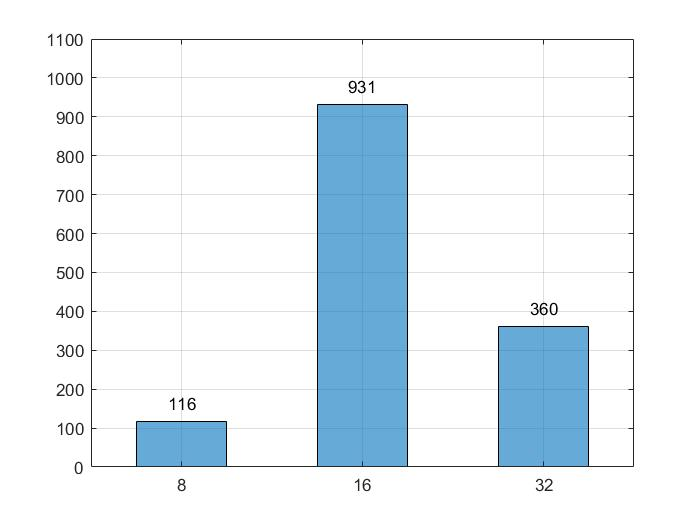
\includegraphics[width=.6\textwidth]{imagenes/chap4/hist_dim_cat.jpg}
    \caption{Histograma que muestra la cantidad de matrices cuyos índices de columna pueden ser representados en 8, 16 y 32 bits%, respectivamente, sin realizar modificaciones a la matriz, determinando los valores máximos, la dimensión de ésta
    .}
    \label{fig:hist_dim_cat}
\end{figure}

En la Figura \ref{fig:hist_dim_cat} se presenta un gráfico con la clasificación de las matrices, dependiendo de si sus índices pueden ser almacenados en cada una de las precisiones. Se puede observar que, del espacio de 1407 matrices estudiadas, quedan catalogadas con 8, 16 y 32 bits, 116, 931 y 360 matrices, respectivamente. Es decir que aproximadamente el $25\%$ de las matrices necesitan 32 bits para ser almacenadas. 

\begin{figure}[h]
    \centering
    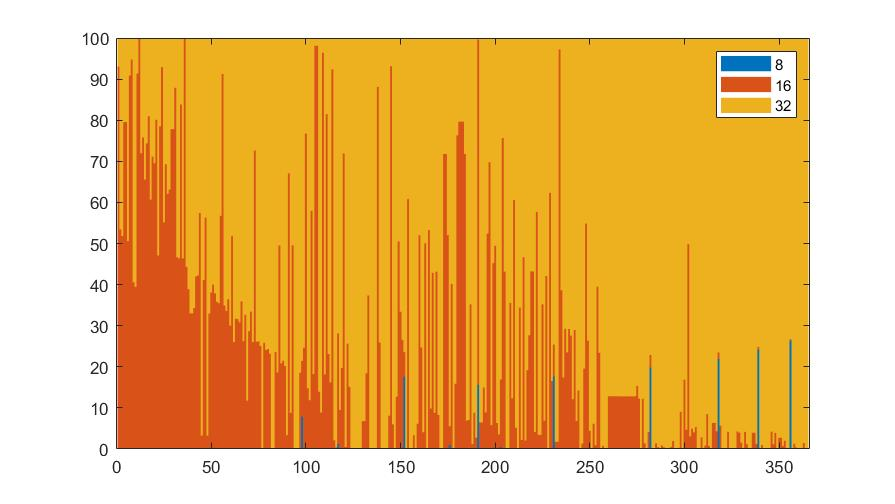
\includegraphics[width=.7\textwidth]{imagenes/chap4/index_bar_row_porc_per_cat_32.jpg}
    \caption{Cada barra del gráfico simboliza una matriz original, que necesita 32 bits para ser representada, y cada componente es el porcentaje de índices máximos por fila que pueden ser representadas con 8, 16 y 32 bits.}
    \label{fig:index_bar_row_porc_per_cat_32}
\end{figure}

En esta y en las secciones posteriores, se estudiarán con mayor foco las matrices que dependiendo de la técnica de compresión analizada, pertenecen a la categoría de 32 bits.  En este sentido, se presenta en la Figura~\ref{fig:index_bar_row_porc_per_cat_32} los resultados para dichas matrices, para observar efectivamente cuántas son las filas que necesitan los 32 bits para ser representadas, o dicho de otra forma, comparar la cantidad de filas que puedan ser representadas con 8 y 16 bits, dentro de las matrices de esta categoría. 
Las barras del gráfico están subdivididas en 3 partes, 
%Las barras del gráfico representan las matrices que pertenecen a la categoría de 32 bits, es decir, aquellas matrices que tienen alguna fila con índice máximo mayor a  $2^{16} - 1$. En particular, cada barra está subdividida en 3 partes,
indicando la proporción de filas de la matriz que pueden ser representadas con las cantidades de bits antes mencionadas. Notar como la división de los porcentajes de filas, está principalmente distribuida, en la mayoría de las matrices, entre 16 y 32 o, en otras palabras, pocas son las matrices que presentan una porción considerable de filas representables con 8 bits (si fueran una cantidad reducida de filas se podrían utilizar formatos híbridos, almacenando esas pocas filas representables con 32 en otra estructura y el resto con precisiones reducidas). Se puede apreciar, que cuanto menor es la cantidad de elementos no nulos, (izquierda del gráfico), menor es la cantidad de filas que necesitan 32 bits para ser almacenadas. A medida que crece dicha cantidad, hacia la derecha, parece aumentar progresivamente la cantidad de filas en 32 bits.



\subsection{Diferencia a la diagonal}\label{diagonal-dif}

Comenzando a evaluar posibles técnicas de compresión enfocadas sobre los índices. %Inspirado en las propuestas de Xu et al.~\cite{Xu2010},
En esta sección se realiza un estudio de la utilización de la diferencia a la diagonal como índice, en lugar del valor de columna original. Para dicho objetivo, es necesario calcular para cada fila de cada una de las matrices, la máxima distancia de un elemento no nulo a la diagonal (en valor absoluto, notar que es equivalente al ancho de banda por fila $\beta (A_i)$). Obtenidos estos valores, se determina cuantos bits son los necesarios  para su almacenamiento y se los clasifica. En este sentido, la Figura~\ref{fig:hist_diag_dist_cat} resume la cantidad de matrices que necesitan 8, 16 y 32 bits para ser almacenadas utilizando esta técnica para representar el índice. 

\begin{figure}[h]
  \centering
  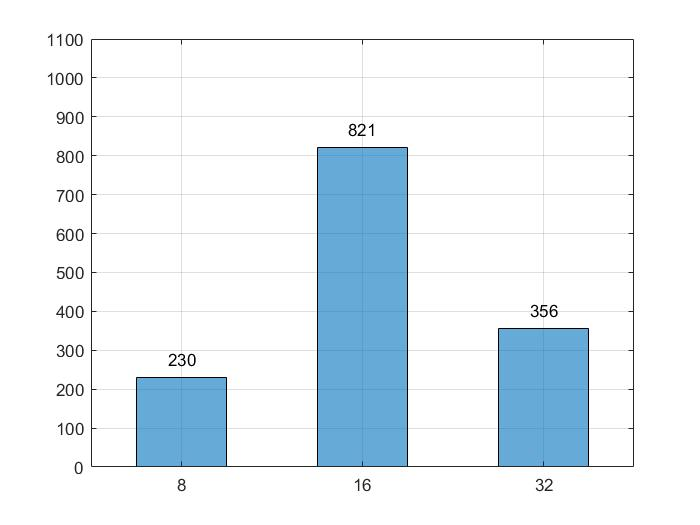
\includegraphics[width=.6\textwidth]{imagenes/chap4/hist_diag_dist_cat.jpg}
  \caption{%Histograma que muestra la clasificación de las matrices originales, según si se les puede aplicar una compresión de índice de columna basados en la distancia a la diagonal con 8, 16 y 32 bits.
  Histograma que muestra la cantidad de matrices cuyos índices de columna expresados como la distancia a la diagonal pueden ser representados en 8, 16 y 32 bits.}
  \label{fig:hist_diag_dist_cat}
\end{figure}%


Notar cómo, a diferencia de la estrategia analizada anteriormente, donde los índices sólo trabajaban con valores positivos, para esta técnica se necesitarán enteros con signo\footnote{Por ejemplo, el índice de una entrada no nula a la derecha de la diagonal tomará valores positivos, mientras que si está a la izquierda negativos.}. En particular, se busca un rango simétrico con respecto a 0, valor que simboliza la diagonal. Se obtienen para 8, 16 y 32 bits los rangos: $[-2^7,2^7]$, $[-2^{15},2^{15}]$ y $[-2^{31},2^{31}]$.



% Se me había ocurrido, modificar un cacho mas el formato, capaz que agrega overhead de descompresión después, pero tener un bit para decir de que lado esta de la diagonal y así tener un bit mas para manejar solo enteros positivos. Básicamente usar el bit de signo, por separado.

\begin{figure}[h!]
    \centering
    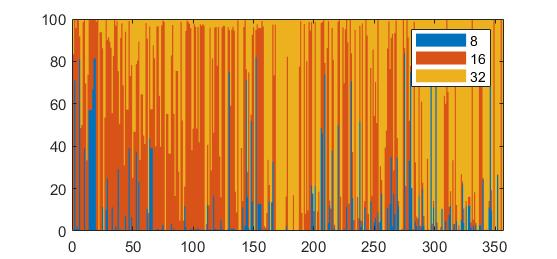
\includegraphics[width=.8\textwidth]{imagenes/chap4/bar_row_porc_per_cat_32.jpg}
    \caption{Cada barra del gráfico simboliza una matriz sin reordenar, que necesita 32 bits para ser representada, y cada componente es el porcentaje de distancias máximas por fila a la diagonal que pueden ser representadas con 8, 16 y 32 bits.}
    \label{fig:bar_row_porc_per_cat_32}
\end{figure}

 En la Figura~\ref{fig:bar_row_porc_per_cat_32}, de manera similar a la anterior sección,  se puede observar un gráfico de barras, del que se desprende que para la gran mayoría de las matrices que pertenecen a la categoría de 32 bits, a medida que crece la cantidad de elementos nulos (hacia la derecha), aumenta el porcentaje de filas en la categoría de 32 bits. También se puede observar cómo decrece el porcentaje de filas en 16 bits, notorio en la porción con menor cantidad de elementos no nulos, agrupada a la izquierda.
 
%  \resumen{Está medio pobre esto creo, no se me opcurre que otra cosa concluir}

\subsection{Diferencia a la diagonal con reordenamiento}\label{diagonal-dif-rcm}

En esta sección, se realiza un análisis del uso de técnicas de reordenamiento. En particular, y siguiendo las ideas propuesta por Xu et al.~\cite{Xu2010}, se aplica la heurística RCM a la técnica de utilizar la diferencia a la diagonal en lugar del índice de columna, presentada en la Sección~\ref{diagonal-dif}.


% \begin{figure}
% \centering
% \begin{subfigure}{.5\textwidth}
%   \centering
%   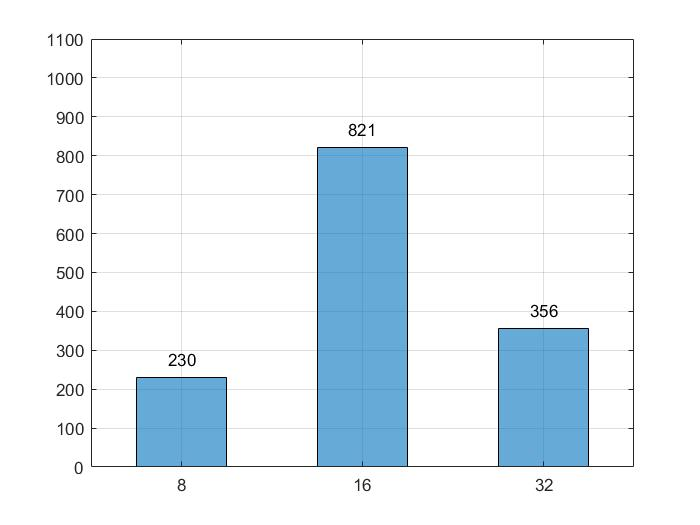
\includegraphics[width=\linewidth]{imagenes/chap4/hist_diag_dist_cat.jpg}
%   \caption{Matrices sin RCM}
%   \label{fig:hist_diag_dist_cat}
% \end{subfigure}%
% \begin{subfigure}{.5\textwidth}
%   \centering
%   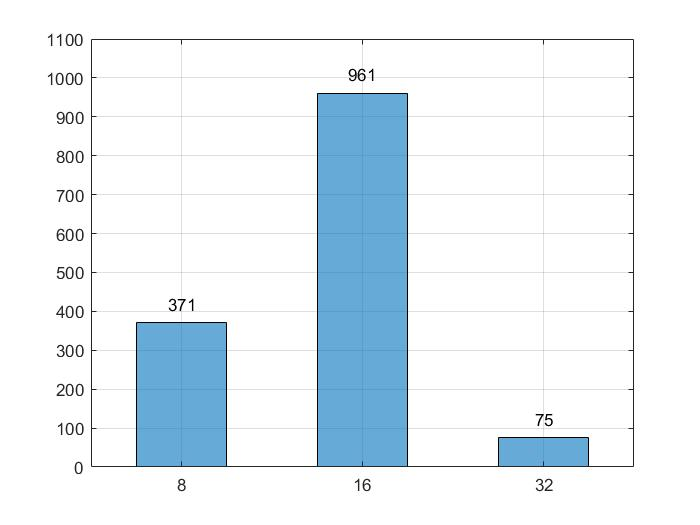
\includegraphics[width=\linewidth]{imagenes/chap4/hist_diag_dist_cat_rcm.jpg}
%   \caption{Matrices con RCM}
%   \label{fig:hist_diag_dist_cat_rcm}
% \end{subfigure}
% \caption{Histogramas donde se muestra la clasificación de las matrices según si se les puede aplicar una compresión de índice de columna basados en la distancia a la diagonal con 8, 16 y 32 bits. Matrices originales~\ref{fig:hist_diag_dist_cat} y con RCM~\ref{fig:hist_diag_dist_cat_rcm}.}
% \label{fig:hist_diag_dist}
% \end{figure}

\begin{figure}[h]
  \centering
  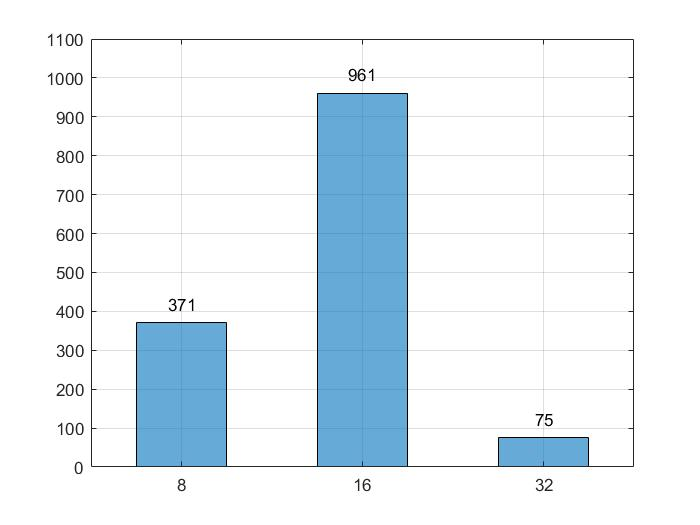
\includegraphics[width=.6\textwidth]{imagenes/chap4/hist_diag_dist_cat_rcm.jpg}
  \caption{
  Histograma que muestra la cantidad de matrices. luego de aplicar RCM, cuyos índices de columna expresados como la distancia a la diagonal pueden ser representados en 8, 16 y 32 bits.
  %Histograma donde se muestra la clasificación de las matrices luego de aplicar RCM, según si se les puede aplicar una compresión de índice de columna basados en la distancia a la diagonal con 8, 16 y 32 bits.
  }
  \label{fig:hist_diag_dist_cat_rcm}
\end{figure}%

Una comparativa de cuántas matrices son representables, utilizando la técnica de distancia a la diagonal, con 8, 16 y 32 bits, con y sin aplicación de reordenamiento, se puede observar en las Figuras \ref{fig:hist_diag_dist_cat} y \ref{fig:hist_diag_dist_cat_rcm}. De las gráficas se deduce que el uso de RCM ofrece importantes beneficios, en especial disminuyendo las matrices representables con 32 bits. Este artilugio, permite pasar de 353 a 63 matrices, del espacio representables con 32 bits, en otras palabras, 290 o el 82\% de dichas matrices se puede almacenar con precisiones menores, siempre y cuando se les aplique un reordenamiento. En el caso de 16 bits, si bien crece el número, muchas de estas son matrices que antes necesitaban 32 bits. De hecho, 154 matrices que necesitaban 16 pasan a 8 bits al aplicar RCM, como se puede observar en la  Figura~\ref{fig:confusion_diag_dist}. Este gráfico, que a los efectos de este proyecto se llamará matriz de composición, es útil para comparar los beneficios de aplicar algún tipo de reordenamiento a una técnica. Cada una de las filas representa la cantidad de matrices que originalmente pueden ser representadas utilizando el número de bits indicada por la fila, a su vez, cada una está subdividida en las categorías a las que van a parar luego de aplicar RCM. Si se la ve por columnas, cada una representa el número de matrices originales que fueron a parar a cada categoría luego de aplicado el reordenamiento obtenido con RCM. %Cuando se accede por columnas, se puede observar la cantidad de matrices en cada precisión luego de reordenar. 
En dicha figura se puede apreciar que, si bien los números del triángulo superior son muy bajos, hay valores por encima de 0 (y uno sólo en 0), indicando que algunas de éstas matrices, en su forma original, pueden ser representadas con una menor cantidad de bits que cuando se les aplica RCM. Para este caso hay 15 matrices que pasan de 8 a 16 bits, y 2 que pasan de 16 a 32. Notar que son cantidades mucho menores a aquellas que si permiten una compresión. De todos modos, evidencia que existen ciertos problemas para los que no sería conveniente aplicar esta técnica de reordenamiento.

\begin{figure}[h]
    \centering
    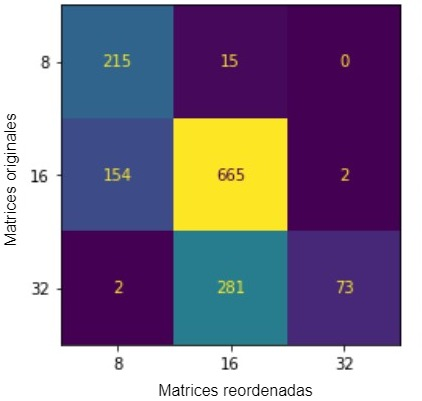
\includegraphics[width=0.4\textwidth]{imagenes/chap4/confusion_diag_dist.jpg}
    \caption{Matriz de composición, muestra en cada fila la distribución de las matrices en cada categoría luego del reordenamiento con RCM, en base a la distancia a la diagonal.}
    \label{fig:confusion_diag_dist}
\end{figure}


\begin{figure}
    \centering
    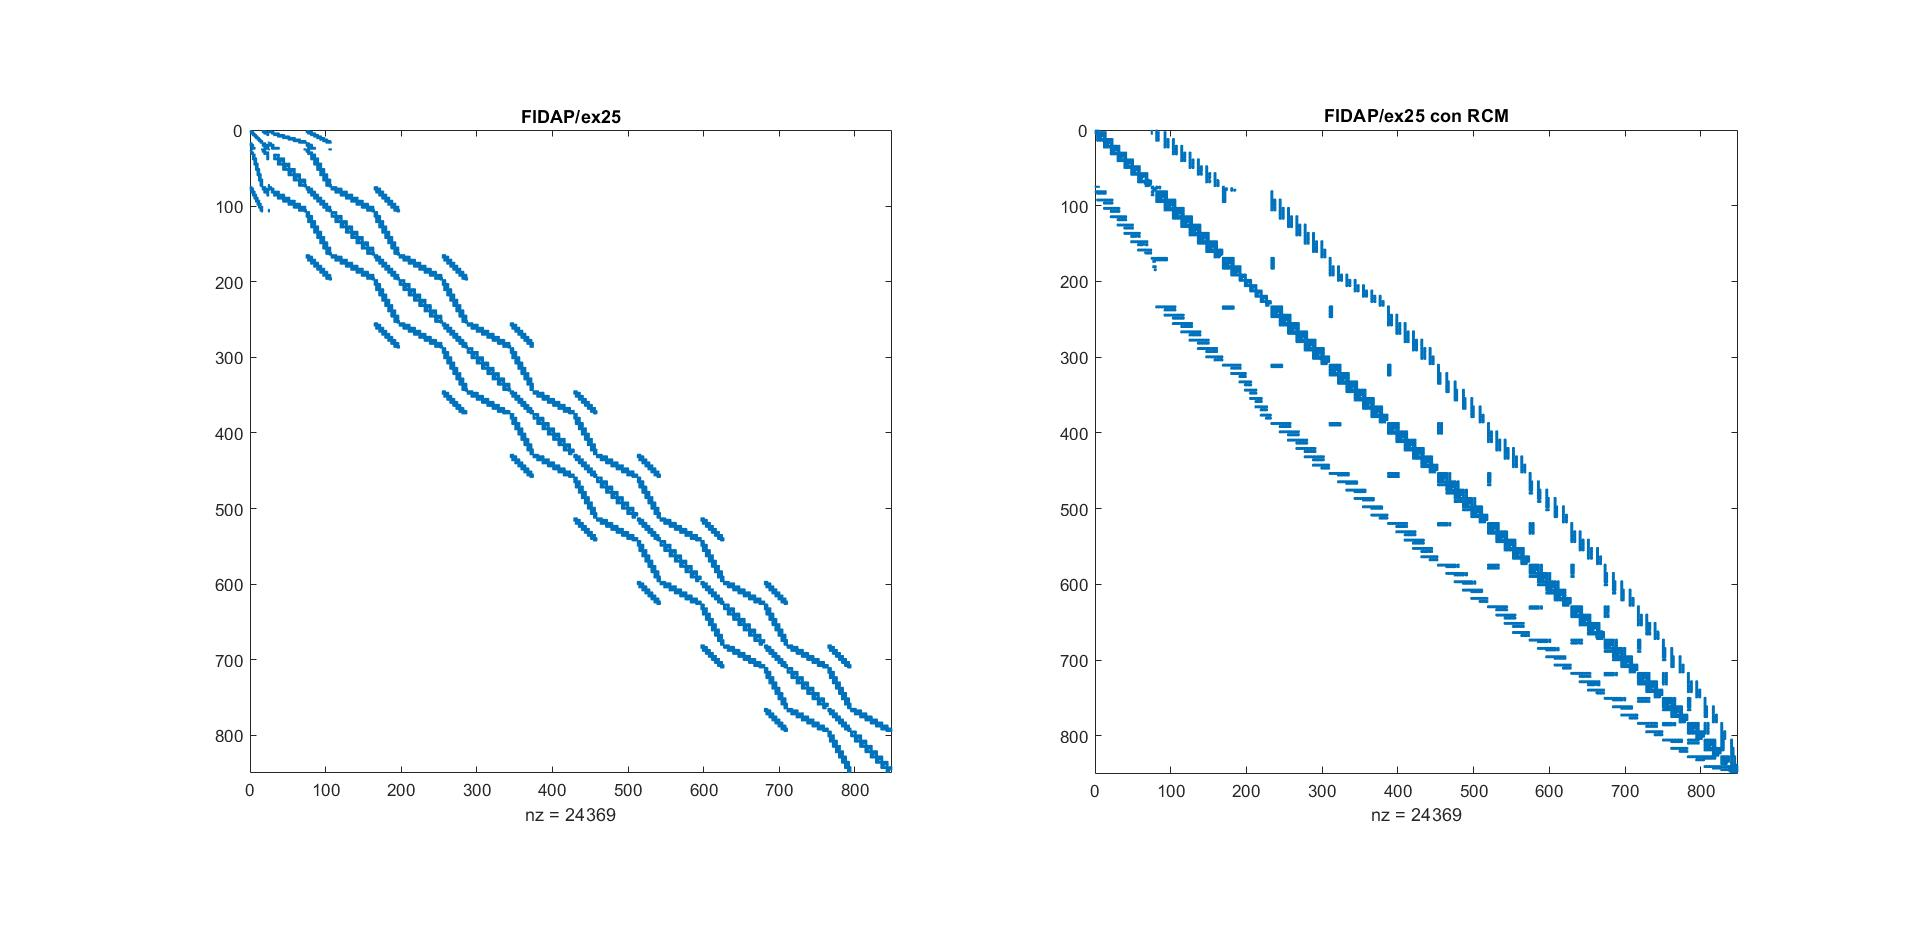
\includegraphics[width=.7\textwidth]{imagenes/chap4/spy_diag_8_to_16.jpg}
    \caption{Ejemplo de matriz que al aplicarle RCM pasa de categoría, de 8 a 16 basado en la diferencia a la diagonal.}
    \label{fig:spy_diag_8_to_16}
\end{figure}


En la Figura~\ref{fig:spy_diag_8_to_16} se presenta el ejemplo de la matriz \texttt{FIDAP/ex25} que pasa, luego de aplicar el reodenamiento generado por RCM, de la categoría de 8 a 16 bits. En particular en el ordenamiento original, las 848 filas eran representables con 8 bits, pasando a tener 475 en esta categoría y 373 en la de 16 bits. Notar la periodicidad de la matriz, estructura que se pierde por  la forma en la que reordena RCM, que pasando de vértices de grados menores a mayores, acaba por producir un leve ensanchamiento en el ancho de banda, rompiendo con la regularidad del ordenamiento original. 



\begin{figure}
    \centering
    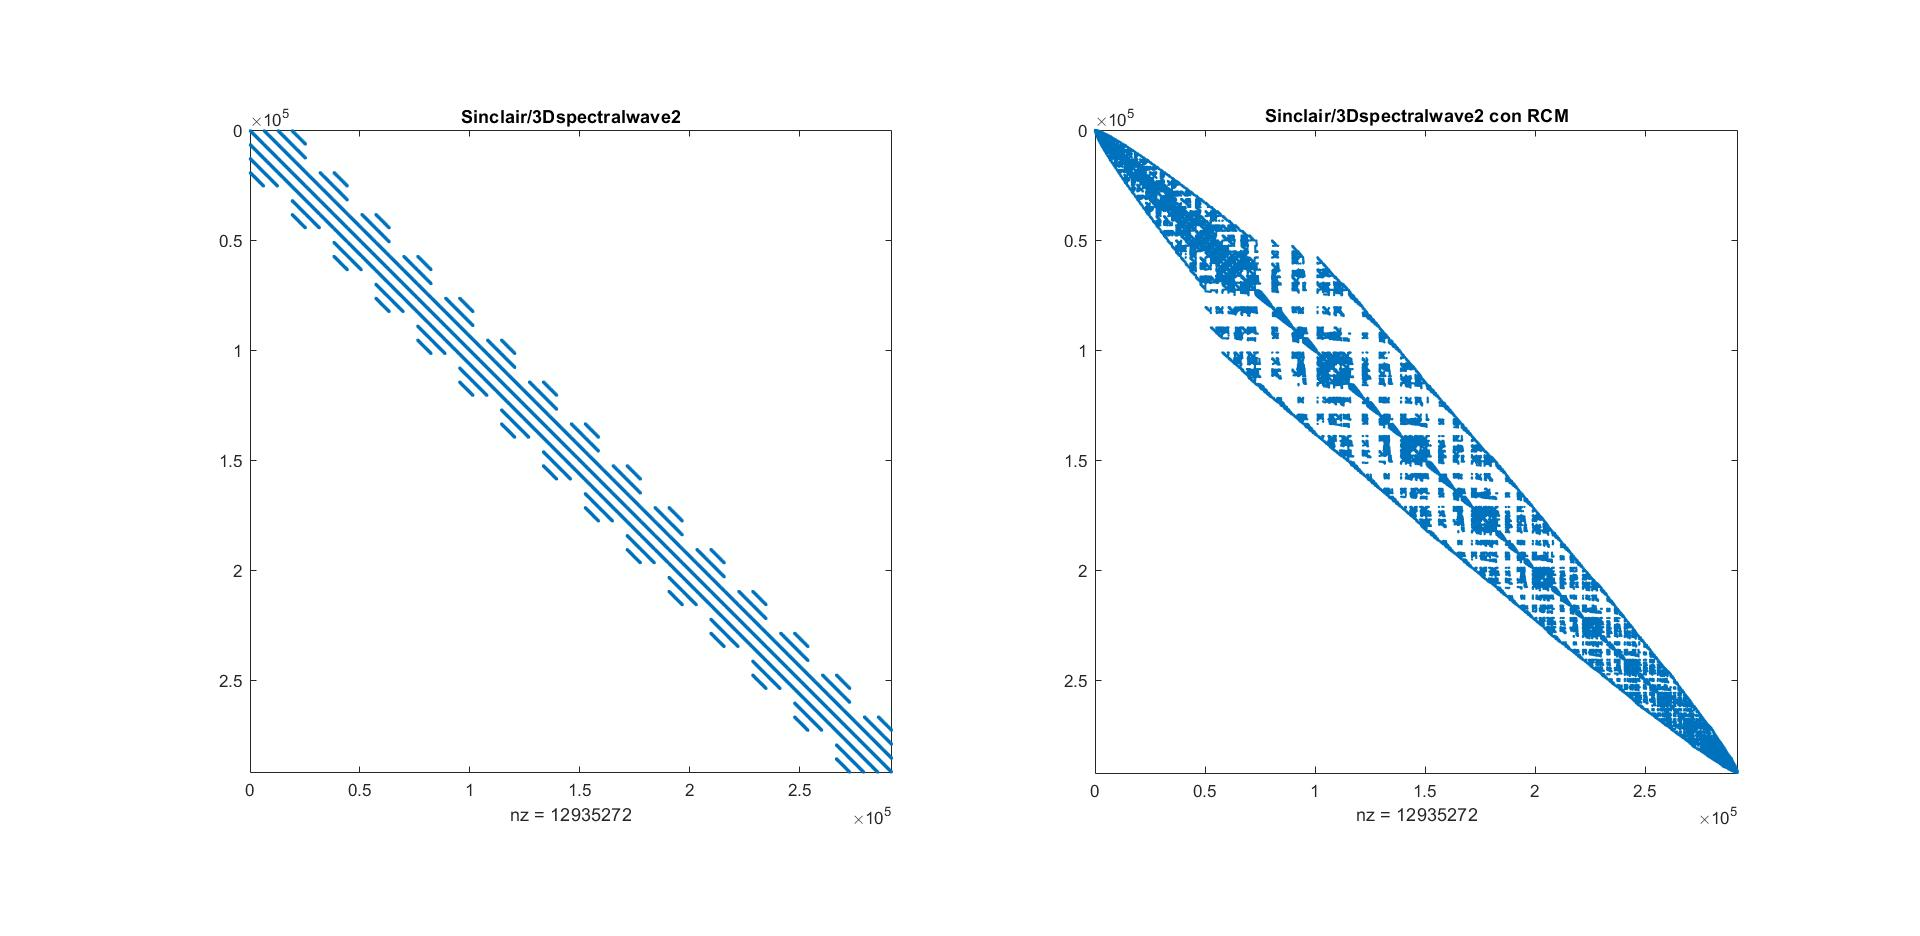
\includegraphics[width=.7\textwidth]{imagenes/chap4/spy_diag_16_to_32.jpg}
    \caption{Ejemplo de matriz que al aplicarle RCM pasa de categoría, de 16 a 32 basado en la diferencia a la diagonal.}
    \label{fig:spy_diag_16_to_32}
\end{figure}

De igual forma, en la Figura~\ref{fig:spy_diag_16_to_32} se plantea un ejemplo de matriz que pasa, en este caso, de 16 a 32 bits. \texttt{Sinclair/3Dspectralwave2} tiene un comportamiento muy similar al ejemplo anterior ante RCM.




% De esto se puede concluir que RCM, puede incluso empeorar el reordenamiento original...... SEGUIR

De esto se puede concluir que en general el uso de las heurísticas de reordenamiento, en particular RCM, permiten ahorrar en el almacenamiento. Sin embargo, es necesario estudiar caso a caso porque en algunos ejemplos de matrices estructuradas, el reordenamiento rompe con dicha estructura llegando a aumentar los requerimientos de almacenamiento, obteniendo resultados contrarios al objetivo.


\begin{figure}[h]
    \centering
    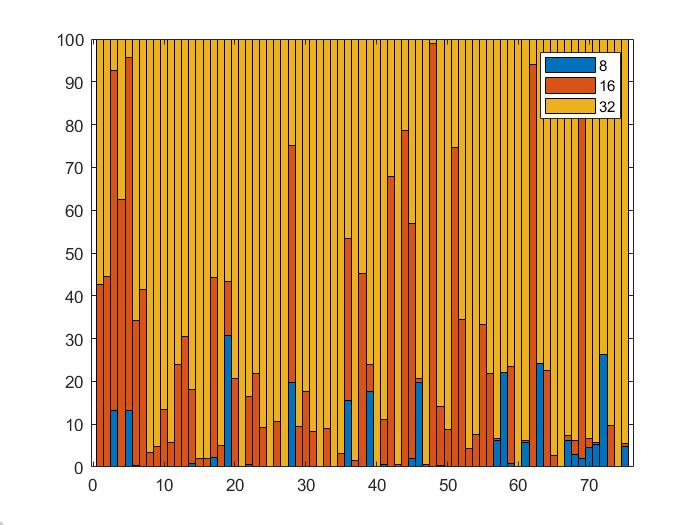
\includegraphics[width=.8\textwidth,height=.5\textwidth]{imagenes/chap4/bar_row_porc_per_cat_32_rcm.jpg}
    \caption{Cada barra del gráfico simboliza una matriz que necesita 32 bits para ser representada luego de aplicar RCM, y cada componente es el porcentaje de distancias máximas por fila a la diagonal que pueden ser representadas con 8, 16 y 32 bits.}
    \label{fig:bar_row_porc_per_cat_32_rcm}
\end{figure}

Buscando profundizar el estudio, tal y como se realizó en los casos anteriores, se toman las matrices representables con al menos 32 bits y se evalúa qué proporción de sus filas, intentando comprimirlas, permiten un cambio de precisión, es decir, una compresión. % Notar que hasta ahora, si una fila necesita 32 bits para ser indexada la matriz entera se considera de dicha categoría.
Resultados que se pueden observar en la Figura~\ref{fig:bar_row_porc_per_cat_32_rcm}, que en general indican que luego de aplicar RCM, las matrices que pertenecen a esta categoría, en su gran mayoría tienen una baja proporción de sus filas representables en precisiones menores que 32 bits. Tampoco se aprecia una correlación importante entre la cantidad de elementos no nulos y la cantidad de filas en precisiones menores.




\subsection{Delta entre índices}\label{delta}

%\resumen{deta\_max por fila}

% Además de clasificar las matrices según la cantidad de bits necesarios para almacenar en un formato donde el índice de columna se cambia por la distancia a la diagonal permitiendo 

Se estudió también, para cada matriz del conjunto definido, el delta o la distancia máxima entre elementos no nulos consecutivos para cada una de las filas y para cada matriz. % Esto, con el objetivo de observar efectivamente cuantas de las matrices dispersas con y sin la aplicación de reordenamientos, son candidatas para una compresión sobre los índices de columna, como la realizada 
Esta idea fue aplicada por Maggioni et al.~\cite{Maggioni2014}, para su formato CoAdELL, presentado de forma breve en el Capítulo~\ref{ch:estado-del-arte}, así como Kourtis et al.~\cite{Kourtis2008} en su formato CSR-DU, entre otros autores~\cite{Tang2013, Willcock2006}.

Al igual que en el estudio de los índices máximos por filas, presentado en la Sección~\ref{col-index-compression}, los valores que toman los índices utilizando este enfoque, son también positivos, notar que el elemento anterior necesariamente tendrá un índice menor, por lo que su resta será positiva.

\begin{figure}[h]
  \centering
  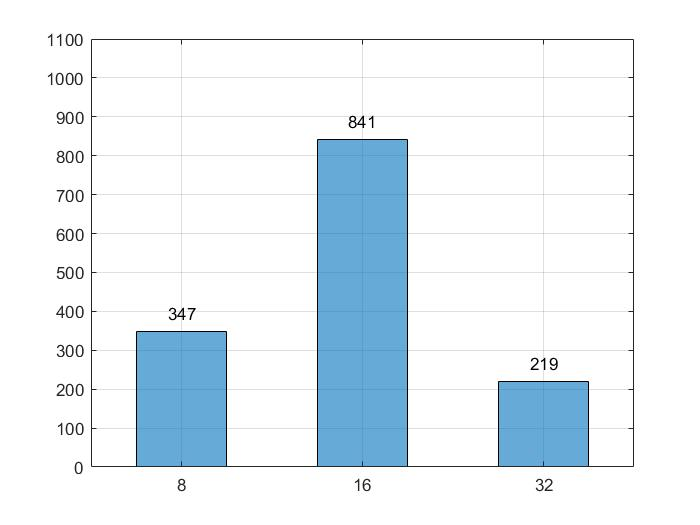
\includegraphics[width=.6\textwidth]{imagenes/chap4/hist_delta_dist_cat.jpg}
  \caption{%Histograma con la clasificación de las matrices, categorizadas según si se les puede aplicar una compresión de índice de columna basados en la distancia al elemento anterior no nulo utilizando 8, 16 y 32 bits
  Histograma que muestra la cantidad de matrices cuyos índices de columna expresados como la distancia al elemento anterior no nulo pueden ser representados en 8, 16 y 32 bits.
  }
  \label{fig:hist_delta_dist_cat}
\end{figure}%

A continuación se presentan algunos de los resultados obtenidos. En la Figura~\ref{fig:hist_delta_dist_cat} se muestra la categorización del espacio de matrices si se representa el índice como la diferencia con el anterior no nulo. Notar que, con respecto a la técnica de diferencia a la diagonal sin reordenar (Figura~\ref{fig:hist_diag_dist_cat}), aplicando esta compresión se obtienen significativamente más matrices en la categoría de 8 bits, mientras que la de 32 bits se ve reducida en un porcentaje similar.% Se mantiene el mismo patrón antes identificado, donde las matrices que pertenecen a esta categoría presentan un gran porcentaje de sus filas representables únicamente en 32 bits.



Cabe destacar que en este caso, los rangos de representación comienzan en cero (a diferencia de los rangos de la parte anterior, que utilizaban representaciones con signo),  permitiendo utilizar 1 bit más dedicado, no al signo, sino a la numeración directamente.

\begin{figure}
    \centering
    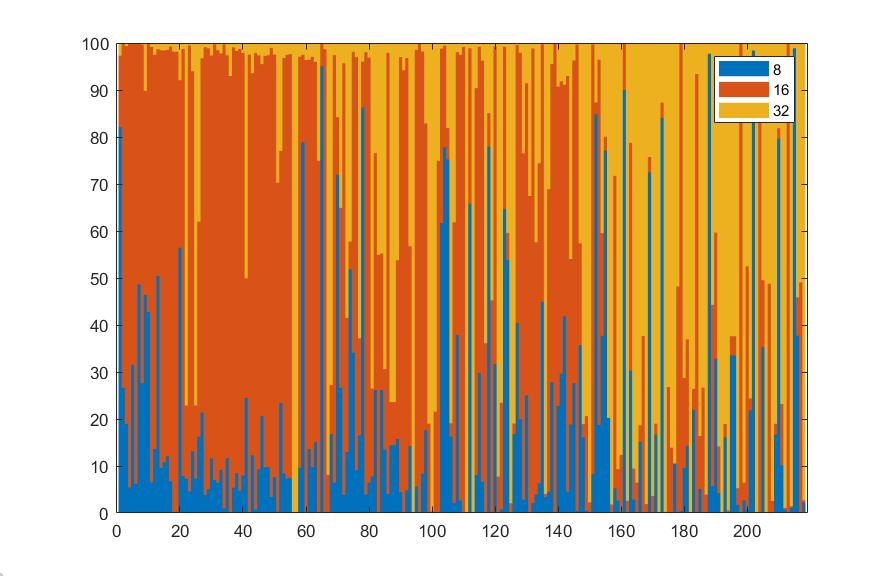
\includegraphics[width=.8\textwidth]{imagenes/chap4/delta_bar_row_porc_per_cat_32.jpg}
    \caption{Cada barra del gráfico simboliza una matriz sin reordenar, que necesita 32 bits para ser representada, y cada componente es el porcentaje de deltas máximos por fila que pueden ser representadas con 8, 16 y 32 bits.}
    \label{fig:delta_bar_row_porc_per_cat_32}
\end{figure}

Similar a lo que se realizó anteriormente, se evalúan las matrices que necesitan 32 bits para ver cuántas filas de esas matrices se pueden representar con 8 y 16 bits. Dicho estudio se resume en la Figura~\ref{fig:delta_bar_row_porc_per_cat_32}. Nuevamente, se puede observar cómo, para las matrices que poseen menores cantidades de \textit{nnz}, ubicadas sobre la izquierda del gráfico, una gran porción presenta muy pocas filas que necesitan 32 bits. A medida que aumenta la cantidad de elementos no nulos de las matrices se puede apreciar, quizás no tan regularmente, un progresivo aumento de las filas en 32 bits.


\subsection{Delta entre índices con reordenamiento}\label{delta-rcm}

\begin{figure}
  \centering
  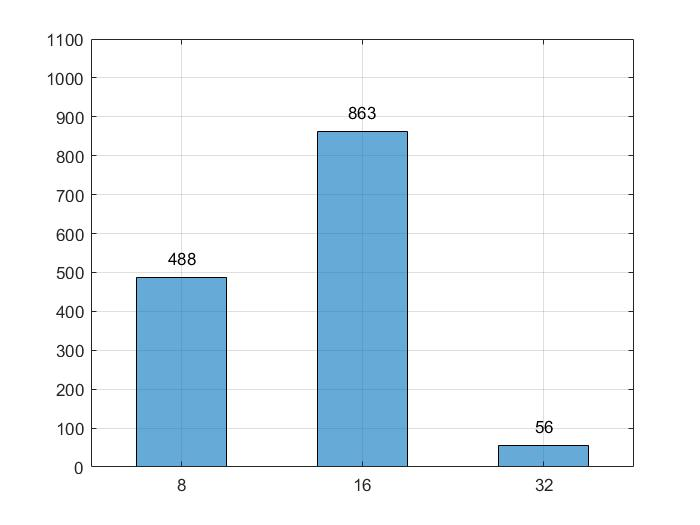
\includegraphics[width=.6\textwidth]{imagenes/chap4/hist_delta_dist_cat_rcm.jpg}
  \caption{%Histograma con la clasificación de las matrices reordenadas con RCM, categorizadas según si se les puede aplicar una compresión de índice de columna basados en la distancia al elemento anterior no nulo utilizando 8, 16 y 32 bits
   Histograma que muestra la cantidad de matrices, luego de aplicar RCM, cuyos índices de columna expresados como la distancia al elemento anterior no nulo pueden ser representados en 8, 16 y 32 bits.
  }
  \label{fig:hist_delta_dist_cat_rcm}
\end{figure}%

Considerando los importantes beneficios de usar RCM para la técnica de sustituir los índices por la diferencia a la diagonal, presentado en \ref{diagonal-dif-rcm}, en este trabajo se propone extender las ideas de Maggioni et al. aplicando RCM pero, en este caso, en conjunto con la codificación delta de forma similar a la propuesta por~\cite{Tang2013}, los resultados se resumen en la Figura~\ref{fig:hist_delta_dist_cat_rcm}.

Para esta conjunción de técnicas, se produce un efecto similar al ocurrido en la Sección~\ref{diagonal-dif-rcm}. Aplicar el reordenamiento de RCM produce resultados mejores, incluso con un impacto más positivo si se comparan los efectos sobre la técnica de la diferencia a la diagonal, obteniendo menores cantidades de matrices en la categoría de 32 bits y mayores en la de 8 bits. Con respecto a las originales con la misma técnica de la distancia al anterior, se logra reducir en aproximadamente  un $75\%$ la cantidad de matrices que se representaban originalmente con 32 bits.


\begin{figure}
    \centering
    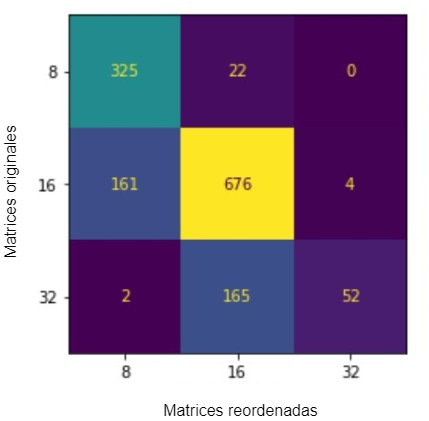
\includegraphics[width=0.4\textwidth]{imagenes/chap4/confusion_delta_dist.jpg}
    \caption{Matriz de composición, muestra en cada fila la distribución de las matrices en cada categoría luego del reordenamiento con RCM, en base a la diferencia con el elemento no nulo anterior.}
    \label{fig:confusion_delta_dist}
\end{figure}


De la misma manera, algunas matrices aumentaron la cantidad de bits necesaria para  poder ser representadas luego de aplicar el reordenamiento de RCM. Estos resultados  se pueden observar en la matriz de composición, presentada en la Figura~\ref{fig:confusion_delta_dist}. En este caso, las relaciones por encima de la diagonal corresponden a 22 matrices que pasan de 8 a 16 bits y 4 que pasan de 16 a 32. Notar que, estos son valores mayores a los obtenidos con la técnica de la diferencia a la diagonal. %Pero, estos resultados no deberían sorprender, dado que con el algoritmo evolutivo se podía apreciar un fenómeno similar, en particular para
\begin{figure}
    \centering
    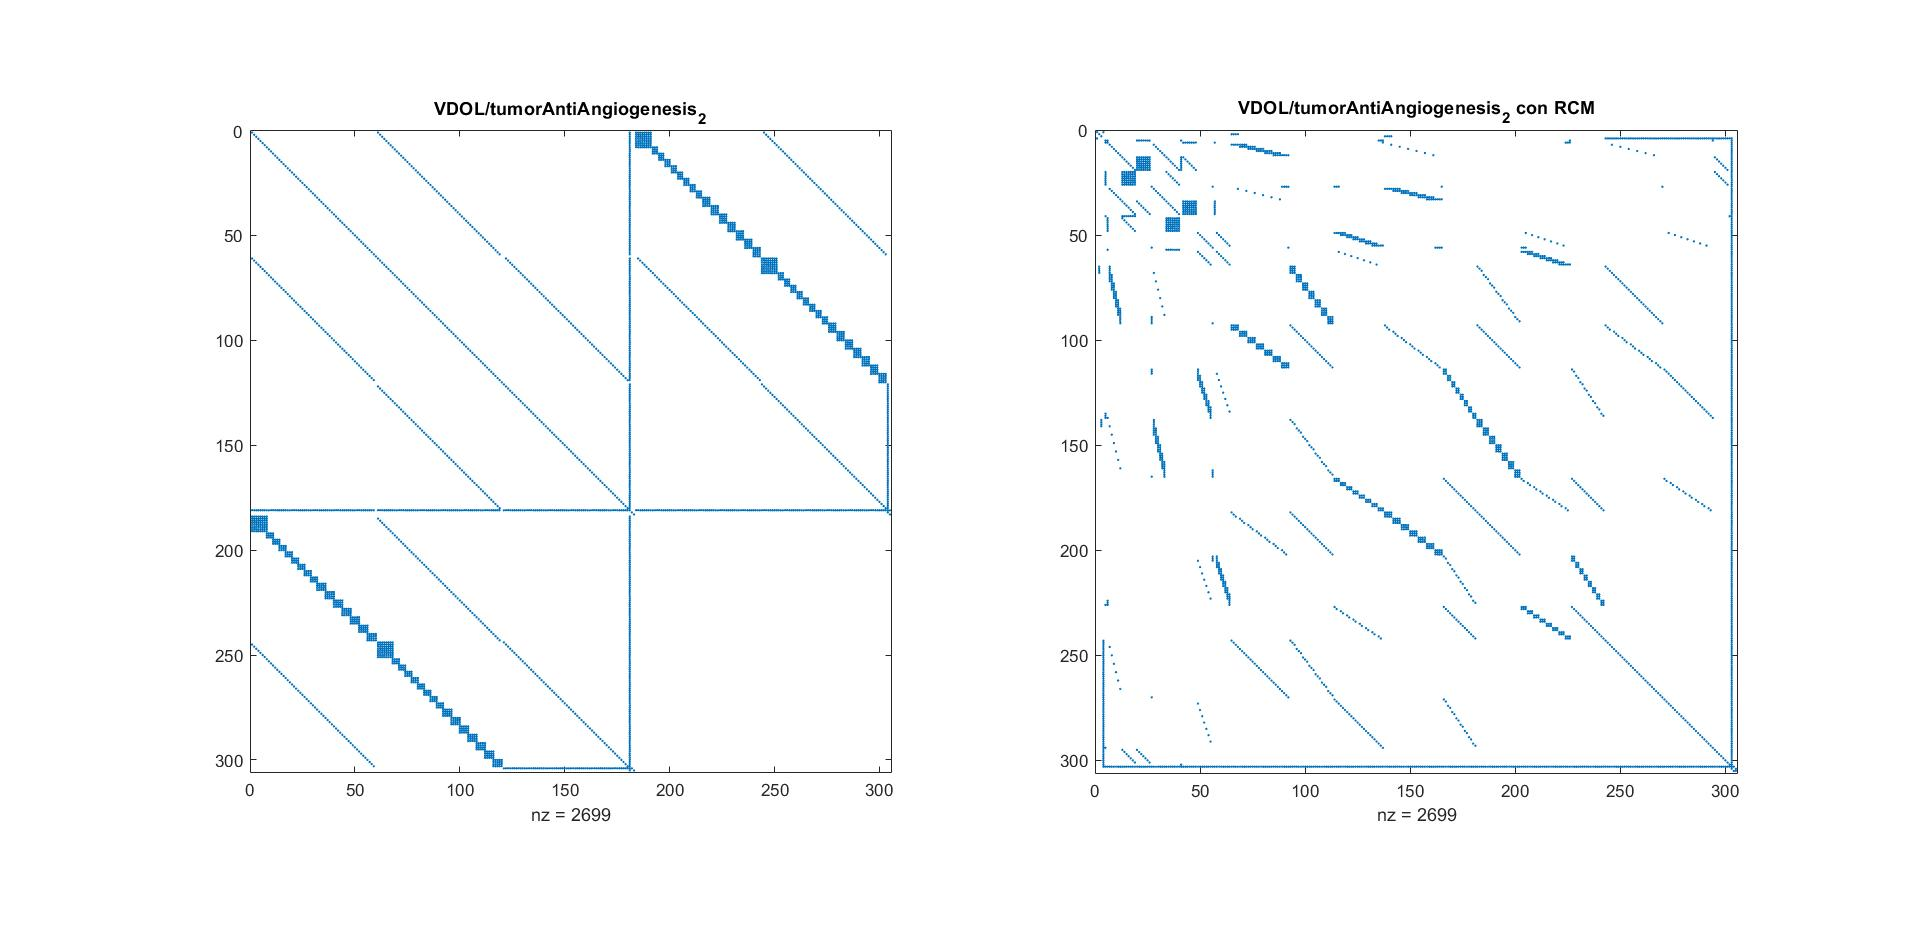
\includegraphics[width=.7\textwidth]{imagenes/chap4/spy_delta_8_to_16.jpg}
    \caption{Ejemplo de matriz que al aplicarle RCM pasa de categoría, de 8 a 16 basado en la diferencia al elemento no nulo anterior.}
    \label{fig:spy_delta_8_to_16}
\end{figure}
\begin{figure}
    \centering
    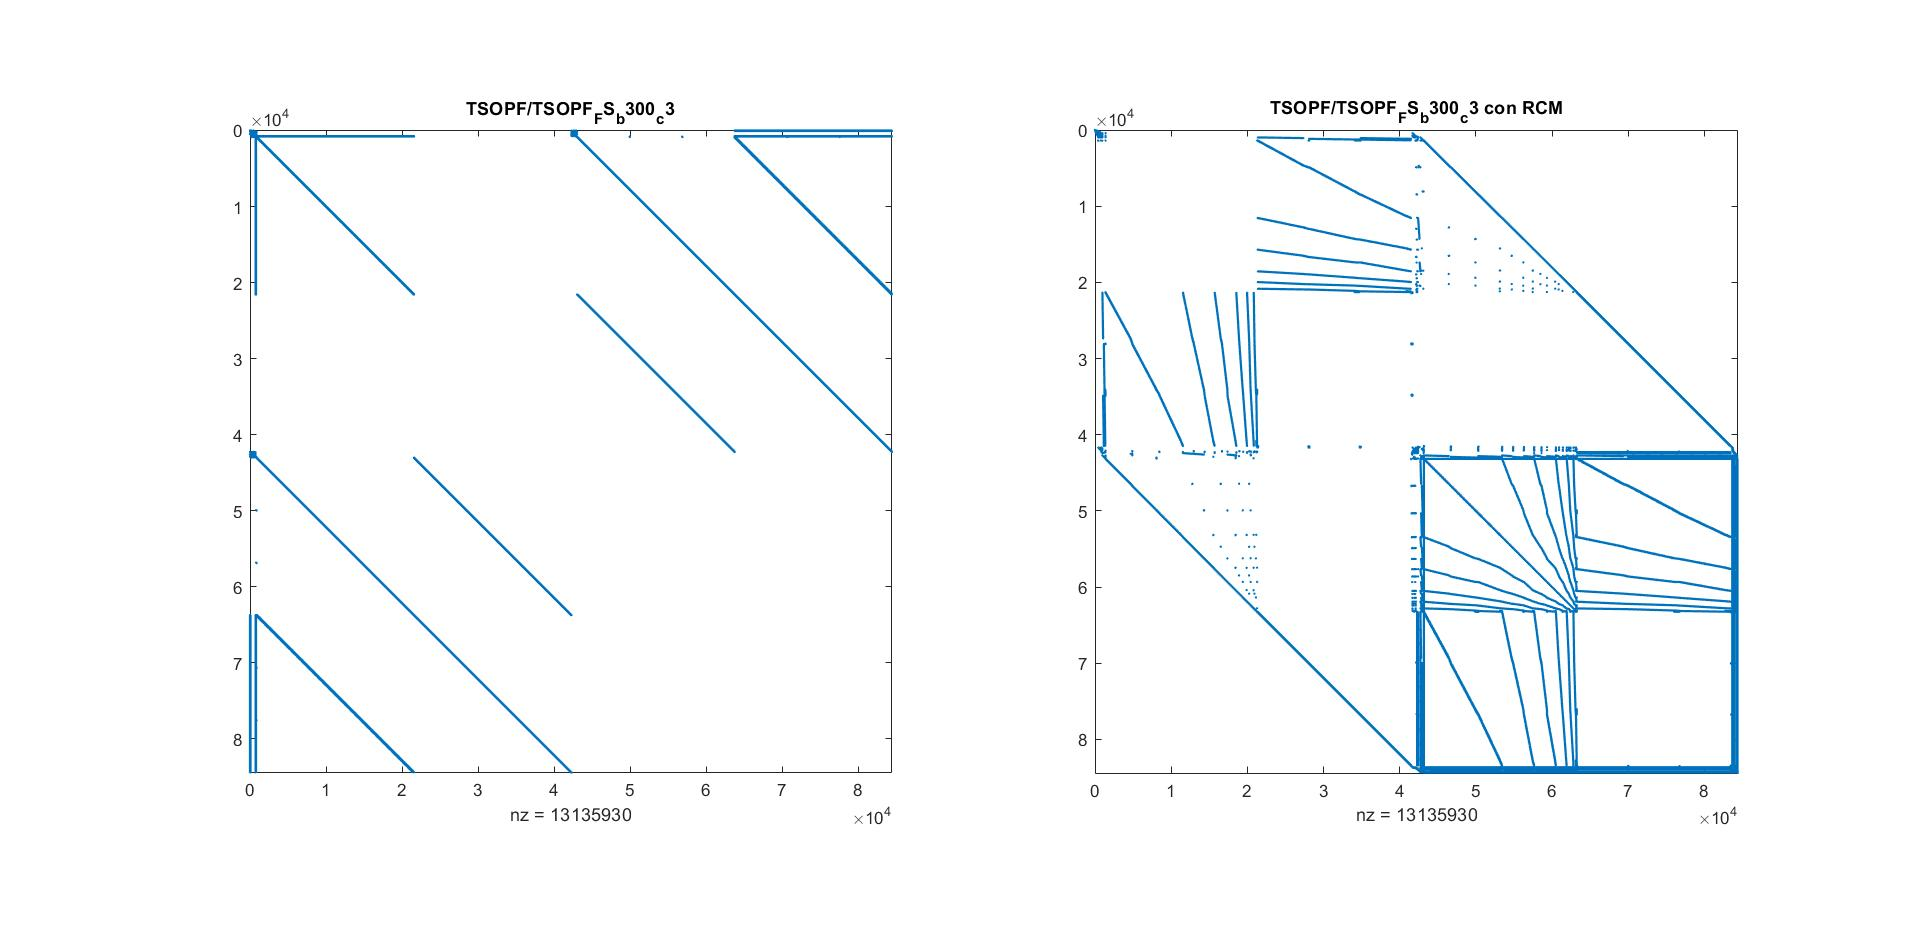
\includegraphics[width=.7\textwidth]{imagenes/chap4/spy_delta_16_to_32.jpg}
    \caption{Ejemplo de matriz que al aplicarle RCM pasa de categoría, de 16 a 32 basado en la diferencia al elemento no nulo anterior.}
    \label{fig:spy_delta_16_to_32}
\end{figure}
En las Figuras~\ref{fig:spy_delta_8_to_16} y \ref{fig:spy_delta_16_to_32} se presentan dos ejemplos de matrices que padecieron esta situación. La Figura~\ref{fig:spy_delta_8_to_16} corresponde a la matriz \texttt{VDOL/tumorAntiAngiogenesis\_2} (la imagen a la izquierda corresponde a la matriz original y la derecha a la misma luego de aplicar RCM), pasando de una distancia máxima de 180 (representable con 8 bits 0-255) entre elementos contiguos en una misma fila, a 283 (con 8 bits no es suficiente). Si bien puede dar la impresión de que, en el desorden, las distancias entre elementos no nulos se acortaron, con un estudio minucioso se  puede observar que no es así, constatando la existencia de filas que tienen distancias mayores a la original.

De igual forma, la Figura~\ref{fig:spy_delta_16_to_32} que representa la matriz~\texttt{TSOPF/TSOPF\_FS\_b300\_c3}, pasando en este caso, de un delta máximo de 42438 representable con 16 bits, a 82215 excediendo dicho rango.



Otro fenómeno que se produce, quizás no se percibe en los gráficos, es el hecho de que muchas matrices luego de aplicarles RCM, si bien no pasan a categorías más grandes, sí sucede que el delta máximo en varios casos es mayor cuando se aplica RCM.


\begin{figure}
    \centering
    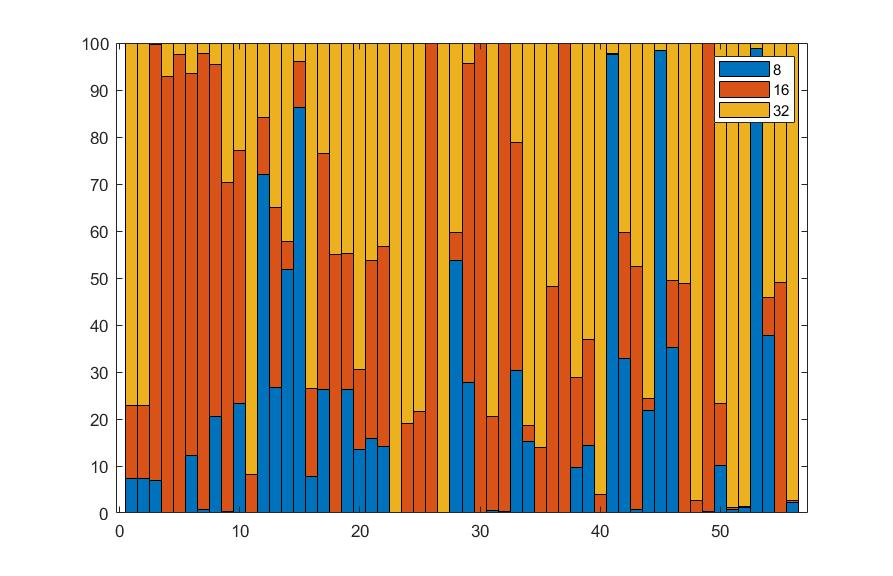
\includegraphics[width=.7\textwidth]{imagenes/chap4/delta_bar_row_porc_per_cat_32_rcm.jpg}
    \caption{Cada barra del gráfico simboliza una matriz que necesita 32 bits para ser representada luego de aplicar RCM, y cada componente es el porcentaje de deltas máximos por fila que pueden ser representadas con 8, 16 y 32 bits.}
    \label{fig:delta_bar_row_porc_per_cat_32_rcm}
\end{figure}

Tal y como se ha realizado en las secciones previas, a continuación se intenta ahondar en las matrices representables con 32 bits, las que poseen posiblemente, (a nuestro criterio mayor) interés. Se presenta en la Figura~\ref{fig:delta_bar_row_porc_per_cat_32_rcm}, un gráfico donde se puede observar, para las 56 matrices ordenadas por cantidad de elementos no nulos, la proporción de filas que pueden ser representadas en las diferentes precisiones. Con un fenómeno muy similar a su contraparte sin ordenar, pero a mucho menor escala, se obtiene un resultado muy variado en la proporción de filas, mientras que las primeras, las de menor \textit{nnz}, presentan pocas filas que necesitan 32 bits. Luego, a medida que aumenta la cantidad de elementos no nulos, paulatinamente crece la proporción de filas que pueden ser representadas sólo con 32 bits.



\subsection{Resumen de la evaluación}

\begin{table}[h]
\centering
\begin{tabular}{|l||r|r|r|}
\hline
         Variante                              & 8   & 16  & 32  \\ \hline\hline
4.3.1. Índice de columna                & 116 & 931 & 360 \\ \hline
4.3.2. Diferencia a la diagonal        & 230 & 821 & 356 \\ \hline
4.3.3. Diferencia a la diagonal con RCM & 371 & 961 & 75  \\ \hline
4.3.4. Delta entre índices              & 347 & 841 & 219 \\ \hline
4.3.5. Delta entre índices con RCM      & 488 & 863 & 56  \\ \hline
\end{tabular}
\caption{Resumen de los resultados de clasificación de las diferentes estrategias evaluadas.}
\label{tab:resumen-resultados}
\end{table}

Para resumir y analizar los datos obtenidos, se presenta en la Tabla~\ref{tab:resumen-resultados} la clasificación del espacio de matrices utilizado, aplicando las diferentes técnicas anteriormente discutidas. 
De ésta se desprenden varios resultados. Probablemente la primera observación que surge analizando la columna de la cantidad de matrices que pertenecen a la categoría de 32 bits, es la reducción de dicha cantidad al aplicar cualquiera de las técnicas propuestas respecto a utilizar los índices originales, incluso sin aplicar reordenamientos como RCM. En el caso de diferencia a la diagonal la reducción no es tan notoria, sólo 4 matrices menos, mientras que utilizando el delta entre índices se obtiene resultados más favorables.

Como segunda observación, las técnicas de reordenamiento abordadas mejoran significativamente la clasificación de las matrices, fenómeno que puede ser observado en la reducción de la cantidad de matrices que se clasifican con 32 bits. 
Esto motiva a continuar profundizando acerca de las técnicas para compresión de matrices aplicando reordenamientos en el futuro.
Otra línea interesante es la exploración de herramientas para optimizar operaciones como la SpMV utilizando estas técnicas, explotando también las características de distintas arquitecturas de hardware.
% Hay que estudiar también, no sólo enfocados en el almacenamiento, herramientas (pensando principalmente en operaciones como SpMV) que sepan explotar dicha estructura (Y también en diferentes arquitecturas), evaluando como afecta, por ejemplo, en términos de accesos a memoria y si existe un cierto \textit{overhead} de descompresión.
A pesar de que RCM no es una heurística específicamente diseñada para reordenar matrices con el objetivo de reducir el espacio de almacenamiento, cabe destacar que los resultados obtenidos, aplicando esta técnica, resultan más que favorables. A esta misma conclusión llegaron múltiples autores en sus investigaciones, tal y como se presenta en el Capítulo~\ref{ch:estado-del-arte}.

 	% Se carga el capítulo 04
  \chapter{Conclusión y trabajo futuro}\label{ch:conclusion}

En este capítulo se detallan las conclusiones más importantes inferidas a través del trabajo realizado en este proyecto de grado. Adicionalmente, se resumen algunas de las posibles líneas de trabajo futuro identificadas que permitirían extender el trabajo.

\section{Conclusiones}
El proyecto tenía por objetivo principal, como se menciona en el Capítulo~\ref{ch:intro}, avanzar en el estudio y comprensión de estrategias de optimización para el uso de matrices dispersas. Poniendo especial foco en el estudio de estrategias de almacenamiento  híbridas y explorando el uso de técnicas de reordenamiento en conjunto con la aplicación de estrategias de precisiones reducidas.
Teniendo en cuenta el objetivo planteado, se desprenden los siguientes objetivos específicos: 
(i) Realizar una actualización del estado del arte del uso de matrices dispersas;
(ii) Actualizar el estado del arte del uso de computación de alta performance (HPC) y en especial, su uso para acelerar la resolución de problemas de álgebra lineal numérica (ALN) dispersa;
(iii) Estudiar estrategias de almacenamiento para matrices dispersas, que apliquen técnicas híbridas, reordenamientos y el uso de múltiples precisiones;
(iv) En base a lo relevado, desarrollar estrategias (formatos, procedimientos, etc.) para matrices dispersas que permitan alcanzar un uso más eficiente de los datos/cómputo.

En primera instancia, se destaca que la ejecución del proyecto permitió cumplir con los objetivos originalmente planteados. En particular, se realizó un relevamiento del estado del arte del uso de matrices dispersas, describiendo varios de los formatos de almacenamiento más conocidos y usados. También se conceptualizó una breve explicación de algunas de las estrategias de reordenamiento más extendidas a la hora de trabajar con matrices dispersas. 
En el mismo marco teórico, se analizó el uso de arquitecturas de HPC y su aplicación para acelerar la resolución de problemas de ALN dispersa, comentando las principales dificultades de operar con este tipo de matrices, y motivando así el estudio de formatos que permitan operar de forma eficiente. 
También se avanzó en la actualización del estado del arte centrado en las técnicas para almacenar y operar con matrices dispersas. Especialmente, aplicando diferentes estrategias que, buscando optimizar ciertos aspectos al operar, trabajan tanto sobre los índices de la matriz, el orden de las filas y columnas, o con los coeficientes de éstas. Como conclusión de esta etapa, se puede destacar que, la gran mayoría de las investigaciones relevadas, tienen su foco en una operación en particular, la SpMV. Y también muchas de ellas están enfocadas en optimizaciones para alguna arquitectura de hardware específica. Se puede notar también que, una cantidad importante de estas investigaciones aplican reordenamientos, ya sea para optimizar cierta propiedad antes de almacenar la matriz, o directamente sobre el formato disperso planteado (por ejemplo para mejorar los accesos a memoria), dejando en claro la importancia de este tipo de enfoques. Se resalta también, que otro conjunto importante de investigaciones buscan disminuir el tráfico de datos entre los distintos niveles de la jerarquía de memoria mediante la reducción de la precisión utilizada, tanto en lo referido a los coeficientes como los índices.

En cuanto al foco principal del trabajo, se proponen y evalúan, en primera instancia, diferentes estrategias para reordenar matrices utilizando heurísticas. En particular, se desarrollaron algoritmos evolutivos, teniendo por objetivo encontrar reordenamientos que permitan explotar técnicas de compresión para lograr un uso eficiente de memoria. Entre los resultados más interesantes que se obtuvieron se puede destacar que, al intentar minimizar la cantidad de diagonales con el algoritmo evolutivo planteado, se logra optimizar también el ancho de banda de la matriz, incluso más que el algoritmo que tenía esta medida por función objetivo.

Por otro lado, se realizó un estudio y discusión sobre los posibles ahorros de memoria al intentar comprimir los índices. Específicamente, se comparan distintas técnicas que explotan el almacenamiento de índices con diferentes precisiones. Para la evaluación experimental se emplean las matrices dispersas, con patrón simétrico, de la colección SSMC, siguiendo un procedimiento sistemático sobre todo el conjunto de prueba y los métodos a evaluar. Este estudio evidencia que, para una gran cantidad de problemas, el abordaje de estos enfoques ofrece importantes mejoras. 
Entre otros resultados se destacan los beneficios al aplicar técnicas alternativas para almacenar los índices, como son el \textit{delta encoding} y la diferencia a la diagonal. Estas mejoras se ven incrementadas si se combinan con la aplicación de las estrategias de reordenamiento, por ejemplo mediante la heurística RCM.

En cuanto a los resultados obtenidos en la evaluación experimental, es necesario enfatizar las importantes reducciones en los requerimientos de almacenamiento alcanzadas. Obteniendo que, en promedio, entre todas las técnicas que no aplican reordenamientos, un 61\% de las matrices analizadas pueden ser almacenadas con 16 bits (entre 9 y 16), y un 16\% pueden ser almacenadas con 8 bits. 
Como aspecto negativo, entre las matrices que requieren 32 bits, no se identifican tendencias que permitan avanzar con el uso parcial de precisiones menores, es decir no hay un número grande de filas que puedan ser almacenadas con una cantidad menor de bits.
%en el espacio de matrices que no admitieron una reducción de precisión (las que pertenecen a la categoría de 32 bits), presente en cada estrategia abordada, es que los índices resultantes quedan clasificados sin lograr una tendencia clara a, por ejemplo, una baja cantidad en 32 bits. Dificultando la posibilidad de intentar trabajar con estrategias híbridas  buscando almacenar la matriz con dos componentes, una con la mayoría de elementos no nulos con precisiones reducidas y los restantes en otra componente con la precisión necesaria. 
Por último, y especialmente destacado, la aplicación de técnicas de reordenamientos, incluso con heurísticas no diseñados para optimizar los parámetros estudiados, ofrecen una importante mejora de las técnicas evaluadas.
En este caso el promedio de las matrices que pueden ser almacenadas con 16 bits sube a 64\% y a 30\% las que se pueden almacenar con 8 bits.



\section{Trabajo futuro}
El desarrollo de este trabajo permitió avanzar en la comprensión de distintas líneas de investigación relacionadas con el almacenamiento de matrices dispersas.
No obstante, existen ciertos puntos importantes vinculados al objetivo del proyecto que, debido al alcance y tiempo, no pudieron se abordados.
A continuación, se detallan algunas de estas ideas que podrían extender el proyecto como trabajo futuro: 
\begin{itemize}
    \item Una línea interesante es desarrollar algoritmos y heurísticas que permitan acercarse más, en cuanto a costos computacionales razonables, a soluciones como las obtenidas por el algoritmo evolutivo de la Sección~\ref{sec:ae}.
    \item Otro aspecto prometedor es implementar y evaluar operaciones matriciales utilizando los formatos propuestos, en particular, para alguna arquitectura de hardware de interés científico.
    \item Por último, sería importante implementar una biblioteca de ALN dispersa capaz de manipular matrices almacenadas con los formatos abordados, operar sobre ellas y así poder estudiar en mayor profundidad los beneficios de estos paradigmas.
\end{itemize} 	% Se carga el capítulo 05
  %\chapter{Evaluación experimental}

En algunas disciplinas, el capítulo Presentación de datos va acompañado del análisis o de la discusión de la información (\textit{Presentación y análisis de los datos}; \textit{Resultados y discusión}), en tanto que en otras, \textit{Presentación}, \textit{Análisis} y \textit{Discusión} son capítulos separados.
El objetivo de esta(s) parte(s) de la tesis es presentar los datos recabados y el análisis realizado a la luz de la bibliografía ya revisada. Se puede incluir la interpretación de los resultados (\textit{Discusión}) a partir del análisis de los datos, o también relacionarlos con estudios relevantes que se entienden pertinentes, aun si estos no se han consignado en los \textit{Fundamentos teóricos}, ya que se entiende que al analizar los datos pueden aparecer algunos que no se enmarcan teóricamente o que no se explican en el encuadre teórico o en estudios ya existentes.

Ahora a modo de ejemplo mencionamos el símbolo de los números reales utilizando el comando \verb|\gls{}| \gls{Real} y el comando \verb|\glssymbol{}| \glssymbol{Real}. Otro ejemplo es mencionar el tensor simétrico de tensiones \gls{sigma}, o un valor escalar  \gls{alph} o un conjunto vacío \gls{emptyset}.

\newpage 


\section{Título de sección}

Ejemplo de tabla

\begin{table}[h!]
\centering
\caption{Leyenda de tabla.}
\label{tab:comp}
\begin{tabular}{|c|c|c|}
  \hline
  $t$ (seg) & $x$(t) & $y$(t)\\
  \hline
  1 & 0.0000 & 0.0001\\
  2 & 0.5000 & 0.2498\\
  3 & 1.0000 & 1.0000\\
  4 & 1.5000 & 2.2403\\
  5 & 2.0000 & 4.0010\\
  6 & 2.5000 & 6.2459\\
  \hline
\end{tabular}
\end{table}

Ejemplo de figura.

\begin{figure}[h!]
\label{fig:comp}
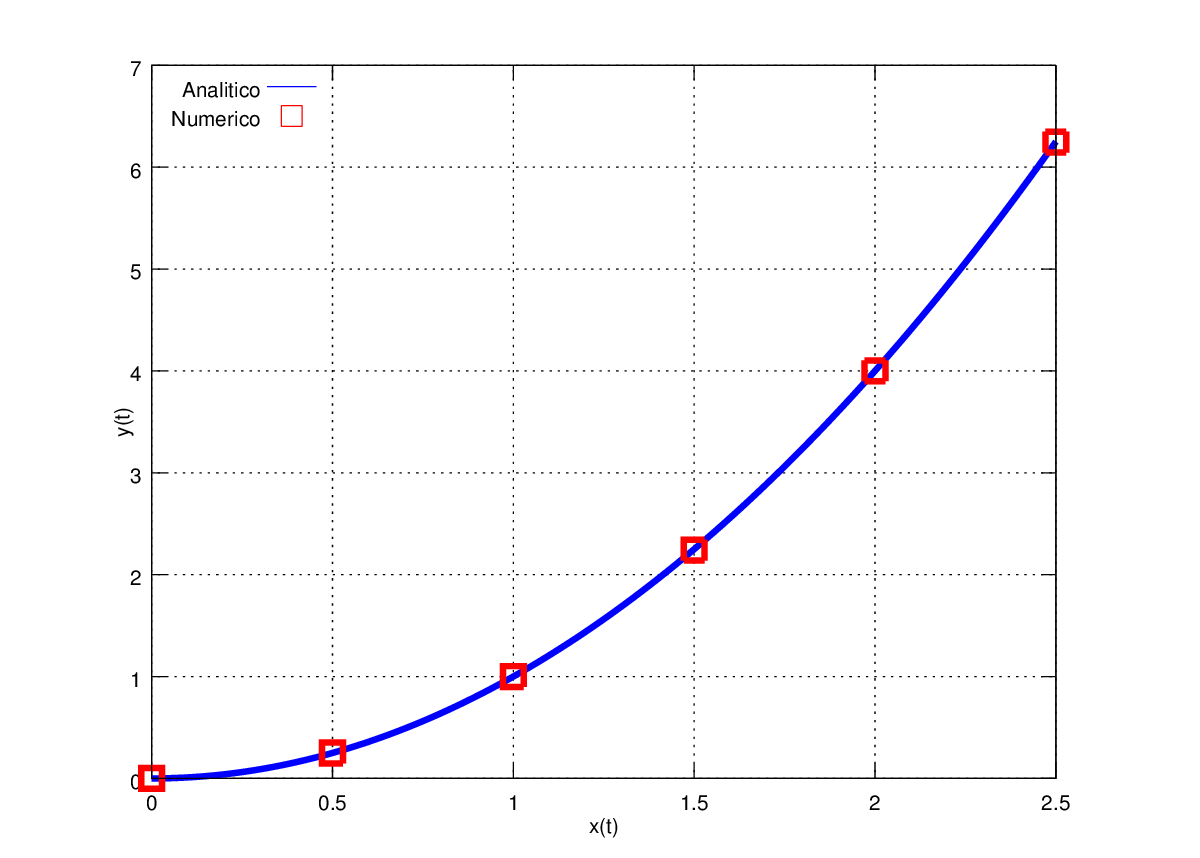
\includegraphics[width=.8\textwidth]{imagenes/chap4/x_vs_y}
\caption{Leyenda de figura.}
\end{figure}
Ejemplo de ecuación:
\begin{equation}
y(x)=x^2
\end{equation}
 	% Se carga el capítulo 06

  % Seguir copiando la linea de arriba para agregar más capítulos.
  
  \backmatter % Comando que generalos apéndices, anexos y bibliografía. NO COMENTAR
  

  \printbibliography[heading=bibintoc]		% Se imprimen las referencias bibliográficas
  \bibend % NO comentar
  % 
%   \glosario 		         % Glosario, NO comentar
  %
  \apenarabicnumbering
  %\apenmatter				 % Apéndices, NO comentar
%  \chapter{Datos procesados}


%  chapter{Imágenes remasterizadas}\label{Ape2}

%  \chapter{Entrevistas desgrabadas}\label{Ape3}

  % Seguir copiando la linea de arriba para agregar más apéndices.
  %
  \anexarabicnumbering
  \anexmatter				 % Anexos, NO comentar
  \chapter{Algoritmo evolutivos}\label{Ane1}

En la computación científica se pueden encontrar numerosos problemas con diferentes complejidades. De forma genérica, estos pueden ser clasificados como problemas ``sencillos'' y problemas ``difíciles''. Esta clasificación depende de la evaluación de la complejidad de los algoritmos capaces de resolver los problemas en diferentes casos.
Formalmente un problema es ``sencillo'', si puede ser resuelto en tiempo polinomial en una computadora determinística. A este tipo de problemas se los llama de clase $\mathcal{P}$. Un problema ``difícil'' o que pertenece a la clase $\mathcal{NP}$,  es aquel que puede ser resuelto en tiempo polinomial pero en una computadora no determinística. (Estos problemas una vez obtenida la solución, son fáciles de verificar, pero difíciles de encontrar.)
En 1971 se planteó la pregunta  ¿si $\mathcal{P}$=$\mathcal{NP}$?  Al día de hoy no se ha podido demostrar si se cumple, se cree que $\mathcal{P} \neq \mathcal{NP}$, siendo uno de los principales desafíos en el campo de la computación.

Problemas $\mathcal{NP}$, son la clase de problemas ``difíciles'' de resolver. Un ejemplo muy común y conocido es el ``Travelling Salesperson Problem'' (TSP) . Este consiste, básicamente, en encontrar un una permutación que represente el recorrido de una serie de ciudades (vértices) conectadas entre si (aristas), de tal forma que todas sean visitadas (sólo una vez), minimizando la distancia total viajada.  A continuación, con el objetivo de observar cuan difícil puede ser resolver este problema de manera óptima. Considerando n ciudades, la dimensión del espacio de búsqueda    (permutaciones) es: $(n-1)!/2$, entonces:
\begin{itemize}
	\item Para $n=10$, hay 181.440 permutaciones posibles.
	\item Para $n=12$ hay 19.958.400 permutaciones posibles.
	\item Para $n=20$ hay 60.822.550.204.416.000 permutaciones posibles.
\end{itemize}

Estos ejemplos evidencian de forma clara, la inviabilidad de buscar una solución por fuerza bruta o una búsqueda exhaustiva.
Entonces, para este tipo de problemas, es necesario utilizar algoritmos de resolución más eficientes que la búsqueda exhaustiva. 

Una clase particular de problemas $\mathcal{NP}$ son los problemas de optimización, los que tienen por objetivo hallar la(s) solucione(s) óptima(s) de un problema (de acuerdo a una función objetivo determinada).  

Existen varias técnicas para ``resolver'' estos problemas, entre ellas: analíticas, métodos exactos (backtracking, programación dinámica, método simplex, etc.), métodos de aproximación, métodos aleatorios y las que se describen con más profundidas en esta sección, heurísticas y metaheurísticas. 
Las heurísticas son métodos de resolución basados en procedimientos conceptualmente simples para encontrar soluciones de buena calidad (no necesariamente hallan la solución óptima) a problemas difíciles, de un modo sencillo y eficiente.

Entonces, por ejemplo, el problema de reordenar una matriz de modo de reducir el ancho de banda (u otra formulación donde se busca la cantidad mínima de diagonales) interpretando la matriz como una matriz de adyacencia, i.e. encontrar un reordenamiento que cumpla lo esperado, es equivalente al problema de dar una permutación de los vértices del grafo asociado a la matriz, de forma de minimizar la función ancho de banda. Como prueba Papadimitriou~\cite{Papadimitriou1976} y discutido brevemente en la Sección~\ref{sec:reordenamientos}, este es un problema $\mathcal{NP}$-completo.

La computación evolutiva engloba un amplio conjunto de técnicas que siguen un mecanismo análogo a los procesos de evolución natural, permite resolver problemas ``difíciles'', similares al planteado, en tiempos y costos computacionales razonables.

\begin{algorithm}[ht]
\begin{minted}{python}
Inicializar(P(0));
generacion = 0;
mientras (no CriterioParada) hacer
    Evaluar(P(generacion));
    Padres = Seleccionar(P(generacion));
    Hijos = Aplicar Operadores Evolutivos(Padres);
    NuevaPoblacion = Remplazar(Hijos,P(generacion));
    generacion++;
    P(generacion) = NuevaPoblacion;
fin
retornar Mejor Solucion Encontrada
\end{minted}
\caption{Esquema genérico de un AE que trabaja sobre una población $P$}
\label{alg:ae-alg}
\end{algorithm}

Un Algoritmo Evolutivo (AE) trabaja sobre una población ($P$) de individuos que representan potenciales soluciones al problema a resolver. En el Algoritmo~\ref{alg:ae-alg} se presenta un esquema general en alto nivel de como trabaja un AE. Formalmente, la representación del individuo es el genotipo, la solución el fenotipo. Otro concepto importante presente en estos algoritmos, es una función de \textit{fitness}, que evalúa los individuos de acuerdo a su adaptación para la resolución del problema.


La estructura general de un AE consiste en un ciclo que conformado por cuatro etapas. 
\begin{enumerate}
    \item \textbf{Evaluación}: se asigna un valor de \textit{fitness} a cada individuo.
    \item \textbf{Selección}: se determinan candidatos adecuados para la generación de la nueva generación.
    \item \textbf{Aplicación de los operadores evolutivos}: se genera un conjunto de descendientes a partir de los individuos seleccionados, mediante operadores que emulan la evolución natural.
    \item \textbf{Reemplazo}: mecanismo que realiza el recambio generacional.
\end{enumerate}

La población $P$ es inicializada, en general, mediante mecanismos aleatorios o guiado por heurísticas específicas.
La aplicación de distintas políticas de selección y reemplazo permiten definir las características del algoritmo evolutivo. Mediante la evaluación de la población basados en su valor de \textit{fitmess} se puede privilegiar los individuos más adaptados (elitismo), aumentar la presión selectiva, incrementar la diversidad genética, etc. Los operadores evolutivos determinan el mecanismo de exploración del espacio de búsqueda del problema, probablemente los más conocidos son los operadores de mutación y recombinación, la utilización de estos establece el tipo de AE. 
Finalmente, la condición de parada determina la finalización del AE, que puede estar basada en el número de generaciones, variación de valores de fitness, estimaciones del error cometido, entre otras.


% Primero inicializar una población de individuos (generación 0), posteriormente evaluarla con la función \textit{fitness} definida. En cada generación se seleccionan los individuos progenitores (los más aptos) y se efectúa el cruzamiento (\textit{crossover}) generando nuevos individuos, llamados hijos. A los hijos, con cierta probabilidad (\texttt{mutation rate}) se les aplica un operador de mutación (\textit{mutation}), que permite la exploración de diferentes secciones del espacio de búsqueda. Si se utiliza un muestreo apicando un remplazo generacional, además de una selección elitista, posteriormente los hijos remplazan a sus progenitores para formar la población de la siguiente generación, y a medida que transcurren las generaciones, se va guardando al individuo más apto según la función \texttt{fitness}. Esto continúa hasta completar una cantidad máxima de generaciones o hasta que se logra cierta condición de parada.

% Este objetivo, modelado por el concepto llamado función \textit{fitness}, es fácilmente modificable intercambiando la dicha función y así obtener permutaciones con otras metas.

% Hasta ahora, se introdujeron directa e indirectamente varios conceptos de importancia en los algoritmos genéticos. Se habló del vector de permutaciones $p$ el cromosoma?, cantidad de diagonales, función fitness. Además de estos, son necesarios otros componentes para definir de forma completa y correcta el algoritmo genético. En otras palabras, a la hora de mapear un problema a un algoritmo genético, se tienen que definir los siguientes componentes:
% \begin{itemize}
%     \item función \textit{fitness}
%     \item cromosoma o individuo
%     \item mutación mutation
%     \item cruzamiento crossover
%     \item population
%     \item mutation rate
%     \item generations
% \end{itemize}
%   \chapter{Evolución GPUs}\label{AneB}

En la Sección \ref{gpu-history} se estudió la evolución de las GPUs desde el punto de vista para el que fueron concebidas en un principio, que era el procesamiento gráfico, sin entrar en detalles muy específicos de cada dispositivo. La arquitectura, bastante consolidada, fue la base de las posteriores generaciones o familias de GPUs que fueron apareciendo en las últimas dos décadas. A continuación se revisa de forma breve, la evolución de las GPUs desde un enfoque arquitectónico de las familias propuestas por NVIDIA, desde Tesla hasta Ampere.

Antes de las arquitecturas unificadas, como se explicó en la  sección anterior, el diseño de las GPUs y sus unidades de cómputo estaban directamente relacionadas con la interfaz de renderizado y despliegue de gráficos. Un ejemplo antes de la llegada de las Tesla, es la GeForce 7900 GTX. Esta tarjeta estaba diseñada básicamente en tres secciones, la primera dedicada al procesamiento de vértices (8 unidades de vertex shaders), 24 fragment shaders y 16 unidades de fragment merging. Este diseño forzaba a tener que estudiar en cuales de las etapas se daban los cuellos de botella de la arquitectura, así lograr cierto equilibro entre las capas. Notar que esta arquitectura es difícilmente escalable.

En cuanto a las aquitecturas de GPUs de NVIDIA, de la era de CUDA, a continuación se detallan las principales características que marcaron y destacaron en cada generación.

\subsubsection*{Tesla}
Entonces NVIDIA resuelve el problema de escalabilidad proponiendo la arquitectura ``unificada'' Tesla. Comparada con las arquitecturas anteriores, ya no hay distinción de capas. Estas son sustituidas por el Stream Multiprocessor (SM), dotado con la capacidad de ejecutar todas las etapas, tareas de vertex, fragment y geometry, sin distinción.


\subsubsection*{Fermi}

\subsubsection*{Kepler}

\subsubsection*{Maxwell}

\subsubsection*{Pascal}

\subsubsection*{Turing}

 










\begin{table}
\centering
\resizebox{\textwidth}{!}{
\begin{tabular}{|l|l|l|l|l|l|} \hline
Año  & Arquitectura & Serie       & Chip   & Dimensión & GPU más representativa  \\\hline \hline
2006 & Tesla        & GeForce 8   & G80   & 90 nm               & 8800 GTX                    \\\hline
2010 & Fermi        & GeForce 400 & GF100 & 40 nm               & GTX 480                     \\\hline
2012 & Kepler       & GeForce 600 & GK104 & 28 nm               & GTX 680                     \\\hline
2014 & Maxwell      & GeForce 900 & GM204 & 28 nm               & GTX 980 Ti                  \\\hline
2016 & Pascal       & GeForce 10  & GP102 & 16 nm               & GTX 1080 Ti                 \\\hline
2018 & Turing       & GeForce 20  & TU102 & 12 nm               & RTX 2080 Ti \\ \hline
\end{tabular}
}
\caption{Diferencias en la arquitectura de las diferentes generaciones de GPUs presentadas por NVIDIA.}\label{tab:gpus-family}
\end{table}


% \subsection{Uso de las GPUs para ALN dispersa}

% Multiplicación matriz vector. Revisar 

% Que mas? De cuSPARSE??

  % Seguir copiando la linea de arriba para agregar más anexos.
  % 
\end{document}

% ===== FIN DEL DOCUMENTO =====